%% Department of Biostatistics Consulting Report Template
%% Version 2.2
%% Sarah R Haile, 2010.12.14
%% Sina Rüeger, 2012.02.20, 2012.12.06 (for STA490)
%% Eva Furrer, 2013.02.01 (for STA490)
%% Isaac Gravestock, 2014.09.01 (Update for RStudio, knitr)
%% Servan Gr?ninger, 2015.12.23
\documentclass[11pt, a4paper]{report}\usepackage[]{graphicx}\usepackage[]{color}
%% maxwidth is the original width if it is less than linewidth
%% otherwise use linewidth (to make sure the graphics do not exceed the margin)
\makeatletter
\def\maxwidth{ %
  \ifdim\Gin@nat@width>\linewidth
    \linewidth
  \else
    \Gin@nat@width
  \fi
}
\makeatother

\definecolor{fgcolor}{rgb}{0.345, 0.345, 0.345}
\newcommand{\hlnum}[1]{\textcolor[rgb]{0.686,0.059,0.569}{#1}}%
\newcommand{\hlstr}[1]{\textcolor[rgb]{0.192,0.494,0.8}{#1}}%
\newcommand{\hlcom}[1]{\textcolor[rgb]{0.678,0.584,0.686}{\textit{#1}}}%
\newcommand{\hlopt}[1]{\textcolor[rgb]{0,0,0}{#1}}%
\newcommand{\hlstd}[1]{\textcolor[rgb]{0.345,0.345,0.345}{#1}}%
\newcommand{\hlkwa}[1]{\textcolor[rgb]{0.161,0.373,0.58}{\textbf{#1}}}%
\newcommand{\hlkwb}[1]{\textcolor[rgb]{0.69,0.353,0.396}{#1}}%
\newcommand{\hlkwc}[1]{\textcolor[rgb]{0.333,0.667,0.333}{#1}}%
\newcommand{\hlkwd}[1]{\textcolor[rgb]{0.737,0.353,0.396}{\textbf{#1}}}%
\let\hlipl\hlkwb

\usepackage{framed}
\makeatletter
\newenvironment{kframe}{%
 \def\at@end@of@kframe{}%
 \ifinner\ifhmode%
  \def\at@end@of@kframe{\end{minipage}}%
  \begin{minipage}{\columnwidth}%
 \fi\fi%
 \def\FrameCommand##1{\hskip\@totalleftmargin \hskip-\fboxsep
 \colorbox{shadecolor}{##1}\hskip-\fboxsep
     % There is no \\@totalrightmargin, so:
     \hskip-\linewidth \hskip-\@totalleftmargin \hskip\columnwidth}%
 \MakeFramed {\advance\hsize-\width
   \@totalleftmargin\z@ \linewidth\hsize
   \@setminipage}}%
 {\par\unskip\endMakeFramed%
 \at@end@of@kframe}
\makeatother

\definecolor{shadecolor}{rgb}{.97, .97, .97}
\definecolor{messagecolor}{rgb}{0, 0, 0}
\definecolor{warningcolor}{rgb}{1, 0, 1}
\definecolor{errorcolor}{rgb}{1, 0, 0}
\newenvironment{knitrout}{}{} % an empty environment to be redefined in TeX

\usepackage{alltt}

\usepackage{verbatim}
\usepackage[vmargin=3cm, hmargin=2cm]{geometry}
\usepackage{url}
\usepackage{hyperref}
\usepackage{fancyhdr}
\usepackage{color}
\usepackage{amsmath, amssymb}
\usepackage{amsthm} %for proof env
\usepackage{multirow}
\usepackage{colortbl}
\usepackage{longtable}
\usepackage{lscape}
\usepackage{subcaption}


\usepackage[authoryear,round]{natbib}
\usepackage[resetlabels]{multibib}
\newcites{packages}{Software packages} %to cite R packages & software
%\usepackage[backend=bibtex]{biblatex}
\usepackage{xspace}
\usepackage{float}

% Use Palatino (URW Palladio) for most of the text\ldots
%\usepackage[sc]{mathpazo}
\linespread{1.05} 
\definecolor{grey}{rgb}{.95,.95,.95}

% And Arial for the rest
%\usepackage[scaled]{helvet}

%set graphics path
\graphicspath{{./fig/}}

% sans serif caption (added by sina)
%\usepackage[font=sf, labelfont={sf}, margin=1cm]{caption}

% fonts for captions the same as for text
\usepackage{caption}

% DEUTSCH
%\usepackage[german]{babel}
%\usepackage[T1]{fontenc}
%\usepackage[latin1]{inputenc}
\usepackage[utf8]{inputenc}
\usepackage{textcomp} %to write degree symbol °

%Use special macros
%% We load package by package and set package relevant parameters.
% Topics are summarized later
%%%%%%%%%%%%%%%%%%%%%%%%%%%%%%%%%%%%%%%%%%%%%%%%%%%%%%%%%%%%%%%%%%%%%%%%
% helping packages
\usepackage{ifthen}
\usepackage{calc}

%%%%%%%%%%%%%%%%%%%%%%%%%%%%%%%%%%%%%%%%%%%%%%%%%%%%%%%%%%%%%%%%%%%%%%%%

\renewcommand{\baselinestretch}{1.2}
\renewcommand{\textfraction}{0}%0.2     % placement of figures
\renewcommand{\topfraction}{1}%.3
\renewcommand{\bottomfraction}{1}%.3
\renewcommand{\floatpagefraction}{1}%.3
\setcounter{bottomnumber}{3}%1

\textwidth6.3in
\textheight9.7in
\topmargin-45pt
\oddsidemargin-.15in
\evensidemargin.15in
\headsep30pt
\headheight15pt
%\footskip20pt


%%%%%%%%%%%%%%%%%%%%%%%%%%%%%%%%%%%%%%%%%%%%%%%%%%%%%%%%%%%%%%%%%%%%%%%%

\usepackage{color}
\definecolor{fgcolor}{rgb}{0.345, 0.345, 0.345}
\definecolor{shadecolor}{rgb}{.97, .97, .97}
\definecolor{messagecolor}{rgb}{0, 0, 0}
\definecolor{warningcolor}{rgb}{1, 0, 1}
\definecolor{errorcolor}{rgb}{1, 0, 0}
\definecolor{DarkBlue}{rgb}{0,0,0.5451}
\definecolor{DarkGreen}{rgb}{0,0.39216,0}
\definecolor{LightYellow}{rgb}{1,1,.8}
\definecolor{orange}{rgb}{.9,0.3445,0}



%%%%%%%%%%%%%%%%%%%%%%%%%%%%%%%%%%%%%%%%%%%%%%%%%%%%%%%%%%%%%%%%%%%%%%%%
\usepackage{afterpage}
\usepackage{natbib}
\usepackage{upquote}

\usepackage[english]{babel}

%%%%%%%%%%%%%%%%%%%%%%%%%%%%%%%%%%%%%%%%%%%%%%%%%%%%%%%%%%%%%%%%%%%%%%%%%%%%%%%
%% maxwidth is the original width if it is less than linewidth
%% otherwise use linewidth (to make sure the graphics do not exceed the margin)
\makeatletter
\def\maxwidth{ %
  \ifdim\Gin@nat@width>\linewidth
    \linewidth
  \else
    \Gin@nat@width
  \fi
}
\makeatother

\newcommand{\hlnum}[1]{\textcolor[rgb]{0.686,0.059,0.569}{#1}}%
\newcommand{\hlstr}[1]{\textcolor[rgb]{0.192,0.494,0.8}{#1}}%
\newcommand{\hlcom}[1]{\textcolor[rgb]{0.678,0.584,0.686}{\textit{#1}}}%
\newcommand{\hlopt}[1]{\textcolor[rgb]{0,0,0}{#1}}%
\newcommand{\hlstd}[1]{\textcolor[rgb]{0.345,0.345,0.345}{#1}}%
\newcommand{\hlkwa}[1]{\textcolor[rgb]{0.161,0.373,0.58}{\textbf{#1}}}%
\newcommand{\hlkwb}[1]{\textcolor[rgb]{0.69,0.353,0.396}{#1}}%
\newcommand{\hlkwc}[1]{\textcolor[rgb]{0.333,0.667,0.333}{#1}}%
\newcommand{\hlkwd}[1]{\textcolor[rgb]{0.737,0.353,0.396}{\textbf{#1}}}%

\usepackage{framed}
\makeatletter
\newenvironment{kframe}{%
 \def\at@end@of@kframe{}%
 \ifinner\ifhmode%
  \def\at@end@of@kframe{\end{minipage}}%
  \begin{minipage}{\columnwidth}%
 \fi\fi%
 \def\FrameCommand##1{\hskip\@totalleftmargin \hskip-\fboxsep
 \colorbox{shadecolor}{##1}\hskip-\fboxsep
     % There is no \\@totalrightmargin, so:
     \hskip-\linewidth \hskip-\@totalleftmargin \hskip\columnwidth}%
 \MakeFramed {\advance\hsize-\width
   \@totalleftmargin\z@ \linewidth\hsize
   \@setminipage}}%
 {\par\unskip\endMakeFramed%
 \at@end@of@kframe}

\renewenvironment{kframe}{%
 \def\at@end@of@kframe{}%
 \ifinner\ifhmode%
  \def\at@end@of@kframe{\end{minipage}}%
  \begin{minipage}{\columnwidth}%
 \fi\fi%
 \def\FrameCommand##1{\hskip\@totalleftmargin \hskip-0\fboxsep
 \colorbox{shadecolor}{##1}\hskip-0\fboxsep
     % There is no \\@totalrightmargin, so:
     \hskip-\linewidth \hskip-\@totalleftmargin \hskip\columnwidth}%
 \MakeFramed {\advance\hsize-\width
   \@totalleftmargin\z@ \linewidth\hsize
   \@setminipage}}%
 {\par\unskip\endMakeFramed%
 \at@end@of@kframe}

\makeatother

% \newenvironment{knitrout}{}{} % an empty environment to be redefined in TeX

\newenvironment{knitrout}{\setlength{\topsep}{0mm}\setlength{\fboxsep}{4mm}}{} 
\usepackage{alltt}

%%%%%%%%%%%%%%%%%%%%%%%%%%%%%%%%%%%%%%%%%%%%%%%%%%%%%%%%%%%%%%%%%%%%%%%%%%%%%%%%%%%%%%%%%%%%%%%%%%%%%%%%%%%%
% from fancyvrb
\usepackage{fancyhdr}
\usepackage{fancyvrb}
\DefineVerbatimEnvironment{Rcode}{Verbatim}{xleftmargin=2em,fontshape=sl,formatcom=\color{DarkGreen}}
\fvset{listparameters={\setlength{\topsep}{0pt}}}

%%%%%%%%%%%%%%%%%%%%%%%%%%%%%%%%%%%%%%%%%%%%%%%%%%%%%%%%%%%%%%%%%%%%%%%%%%%%%%%%%%%%%%%%%%%%%%%%%%%%%%%%%%%%%
\usepackage{float}
\usepackage{graphicx}
\usepackage[margin=2em,labelfont=bf]{caption}



%%%%%%%%%%%%%%%%%%%%%%%%%%%%%%%%%%%%%%%%%%%%%%%%%%%%%%%%%%%%%%%%%%%%%%%%
\usepackage[pdftex,plainpages=false,pdfpagelabels,pagebackref=true,colorlinks=true,pdfpagemode=UseOutlines]{hyperref}


%%%%%%%%%%%%%%%%%%%%%%%%%%%%%%%%%%%%%%%%%%%%%%%%%%%%%%%%%%%%%%%%%%%%%%%%
% now math stuff and other details...
\usepackage{amsmath,amsthm,amssymb}

\newtheorem{pro}{Property}[chapter]
\theoremstyle{definition}
\newtheorem{des}{Definition}[chapter]
\newtheorem{bsp}{Example}[chapter]
\newtheorem{rem}{Remark}[chapter]

%\newcommand{\widebar}[1]{\overline{#1}}
\newcommand*\widebar[1]{%
  \vbox{%
    \hrule height 0.5pt%     % Line above with certain width
    \kern0.5ex%             % Distance between line and content
    \hbox{%
      \kern-0.1em%           % Distance between content and left side of box, negative values for lines shorter than content
      \ifmmode#1\else\ensuremath{#1}\fi%  % The content, typeset in dependence of mode
      \kern-0.1em%      % Distance between content and left side of box, negative values for lines shorter than content
    }% end of hbox
  }% end of vbox
}
\def\ds{\displaystyle}

\newcommand{\rr}[1]{{\ttfamily\slshape\color{DarkGreen} #1}}

\makeatletter


% clever trick to circumvent potential redefines after loading packages:
% \providecommand{\something}{}  % if it does not exist, it creates it.
%      has same syntax as \newcommand
% \renewcommand{\something}{....}
% TUGboat 29(2)


\makeatletter
%umdefinierung exisitierender befehle
\let\oldH\H
\let\oldL\L
\let\oldO\H
\let\oldS\S
\let\olda\a
\let\oldb\b
\let\oldc\c
\let\oldd\d
\let\oldk\k
\let\oldv\v
\let\oldl\l
\let\oldt\t
\let\oldu\u
\let\oldIJ\IJ
\let\oldP\P
\let\P\relax
\let\oldnorm\|

%\DefineVerbatimEnvironment{CodeInput}{Verbatim}{fontshape=sl}
%\DefineVerbatimEnvironment{CodeOutput}{Verbatim}{}

\def\endrem{\hfill$\clubsuit$\\}
\def\endbibrem{\hfill$\spadesuit$\\}


\renewcommand{\|}{|\!|}         % closer norm
\newcommand{\T}{{}^{\top}}%\newcommand{\T}{{}^{\mathsf{T}}}
\newcommand\code[1]{{\tt#1}}
\DeclareMathOperator{\tol}{T}                       % Tolerance reagion

\def\spam{\code{spam}}
\def\R{{\sf R}}
\def\fields{\code{fields}}


\newcounter{algo}
\newenvironment{algorithm}{%
  \begin{list}{
      (\arabic{algo})
    }{
      \usecounter{algo}
    }%
}{
  \end{list}
}

% some text abbreviation
\newcommand{\GLS}{\text{GLS}}
\newcommand{\RR}{\text{RR}}
\newcommand{\OR}{\text{OR}}
\newcommand{\WLS}{\text{WLS}}
\newcommand{\MLE}{\text{MLE}}
\newcommand{\OLS}{\text{OLS}}
\newcommand{\MAE}{\text{MAE}}
\newcommand{\MAD}{\text{MAD}}
\newcommand{\RMSE}{\text{RMSE}}

\newcommand{\ii}{\text{\i}}

\newcommand{\Bin}{\cB\mathit{\!i\!n}}
\newcommand{\Beta}{\cB\mathit{\!e\!t\!a}}
\newcommand{\Pois}{\cP\mathit{\!o\!i\!s\!s\!o\!n}}
\newcommand{\Exp}{\cE\mathit{\!x\!p}}


\DeclareMathOperator*{\argmin}{argmin}
\DeclareMathOperator*{\argmax}{argmax}
\DeclareMathOperator{\diag}{diag}
\DeclareMathOperator{\diam}{diam}
\DeclareMathOperator{\card}{card}
\DeclareMathOperator{\cov}{Cov}                   
\DeclareMathOperator{\corr}{Corr}                 
\DeclareMathOperator{\var}{Var}                   
\DeclareMathOperator{\trace}{tr}                  
\DeclareMathOperator{\E}{E}                       
\DeclareMathOperator{\P}{P}                       
\DeclareMathOperator{\pred}{p}
\DeclareMathOperator{\vect}{vec}                  
\DeclareMathOperator{\vech}{vech}                 
\DeclareMathOperator{\rank}{rank}                 
\DeclareMathOperator{\e}{e}                       
%\DeclareMathOperator{\cv}{CV}                     
\DeclareMathOperator{\GCV}{GCV}                     
\DeclareMathOperator{\CV}{CV}                     
\DeclareMathOperator{\BLUP}{BLUP}                 
\DeclareMathOperator{\MSE}{MSE}                   
\DeclareMathOperator{\MS}{MS}                   
\DeclareMathOperator{\df}{df}                   
\DeclareMathOperator{\bias}{bias}                   
\DeclareMathOperator{\eig}{eig}                   
\DeclareMathOperator{\Prec}{Prec}
\DeclareMathOperator{\mode}{mode}
\renewcommand{\SS}{\text{SS}}
\renewcommand{\d}{\mathsf{\,d}}

\def\arctanh{\qopname\relax o{arctanh}}  % as in amsopn
\newcommand{\bigo}{\cO}
\newcommand{\lito}{\text{\scriptsize{$\cO$}}}
\newcommand{\cdfPhi}{\itPhi}
\newcommand{\simiid}{\stackrel[]{\text{iid}}{\sim}}
\newcommand{\ml}{_\text{ML}}

\newcommand*{\stack@relbin}[3][]{%
  \mathop{#3}\limits
  \toks@{#1}%
  \edef\reserved@a{\the\toks@}%
  \ifx\reserved@a\@empty\else_{#1}\fi
  \toks@{#2}%
  \edef\reserved@a{\the\toks@}%
  \ifx\reserved@a\@empty\else^{#2}\fi
  \egroup
}%
\renewcommand*{\stackrel}{\mathrel\bgroup\stack@relbin}
\newcommand*{\stackbin}{\mathbin\bgroup\stack@relbin}


% Kalligraphischer Schriftsatz
\newcommand{\cA}{{\cal{A}}}
\newcommand{\cB}{{\cal{B}}} 
\newcommand{\cC}{{\cal{C}}}
\newcommand{\cD}{{\cal{D}}} 
\newcommand{\cE}{{\cal{E}}}
\newcommand{\cF}{{\cal{F}}}
\newcommand{\cG}{{\cal{G}}}
\newcommand{\cH}{{\cal{H}}}
\newcommand{\cI}{{\cal{I}}}
\newcommand{\cJ}{{\cal{J}}}
\newcommand{\cK}{{\cal{K}}}
\newcommand{\cL}{{\cal{L}}}
\newcommand{\cM}{{\cal{M}}} 
\newcommand{\cN}{{\cal{N}}}
\newcommand{\cO}{{\cal{O}}} 
\newcommand{\cP}{{\cal{P}}}
\newcommand{\cQ}{{\cal{Q}}} 
\newcommand{\cR}{{\cal{R}}} 
\newcommand{\cS}{{\cal{S}}} 
\newcommand{\cT}{{\cal{T}}}
\newcommand{\cU}{{\cal{U}}}
\newcommand{\cV}{{\cal{V}}}
\newcommand{\cW}{{\cal{W}}}
\newcommand{\cX}{{\cal{X}}} 
\newcommand{\cY}{{\cal{Y}}}
\newcommand{\cZ}{{\cal{Z}}} 


\newcommand{\IA}{{\mathbb{A}}}
\newcommand{\IB}{{\mathbb{B}}}
\newcommand{\IC}{{\mathbb{C}}}
\newcommand{\ID}{{\mathbb{D}}}
\newcommand{\IE}{{\mathbb{E}}}
\newcommand{\IF}{{\mathbb{F}}}
\newcommand{\IG}{{\mathbb{G}}}
\newcommand{\IH}{{\mathbb{H}}}
\newcommand{\II}{{\mathbb{I}}}
%\newcommand{\IJ}{{\mathbb{J}}}
\newcommand{\IK}{{\mathbb{K}}}
\newcommand{\IL}{{\mathbb{L}}}
\newcommand{\IM}{{\mathbb{M}}}
\newcommand{\IN}{{\mathbb{N}}}
\newcommand{\IO}{{\mathbb{O}}}
\newcommand{\IP}{{\mathbb{P}}}
\newcommand{\IQ}{{\mathbb{Q}}}
\newcommand{\IR}{{\mathbb{R}}}
\newcommand{\IS}{{\mathbb{S}}}
\newcommand{\IT}{{\mathbb{T}}}
\newcommand{\IU}{{\mathbb{U}}}
\newcommand{\IV}{{\mathbb{V}}}
\newcommand{\IW}{{\mathbb{W}}}
\newcommand{\IX}{{\mathbb{X}}}
\newcommand{\IY}{{\mathbb{Y}}}
\newcommand{\IZ}{{\mathbb{Z}}}


% fette griechische kleinbuchstaben
\newcommand{\balpha}{{\boldsymbol{\alpha}}}
\newcommand{\bbeta}{{\boldsymbol{\beta}}}
\newcommand{\bgamma}{{\boldsymbol{\gamma}}}
\newcommand{\bdelta}{{\boldsymbol{\delta}}}
\newcommand{\blambda}{{\boldsymbol{\lambda}}}
\newcommand{\bepsilon}{{\boldsymbol{\epsilon}}}
\newcommand{\bvarepsilon}{{\boldsymbol{\varepsilon}}}
\newcommand{\bzeta}{{\boldsymbol{\zeta}}}
\newcommand{\bfeta}{{\boldsymbol{\eta}}}  %  <----- exception !
\newcommand{\btheta}{{\boldsymbol{\theta}}{}}
\newcommand{\bvartheta}{{\boldsymbol{\vartheta}}}
\newcommand{\biota}{{\boldsymbol{\iota}}}
\newcommand{\bkappa}{{\boldsymbol{\kappa}}}
\newcommand{\bmu}{{\boldsymbol{\mu}}}
\newcommand{\bnu}{{\boldsymbol{\nu}}}
\newcommand{\bxi}{{\boldsymbol{\xi}}}
\newcommand{\bpi}{{\boldsymbol{\pi}}}
\newcommand{\bvarpi}{{\boldsymbol{\varpi}}}
\newcommand{\brho}{{\boldsymbol{\rho}}}
\newcommand{\bvarrhoi}{{\boldsymbol{\varrho}}}
\newcommand{\bsigma}{{\boldsymbol{\sigma}}}
\newcommand{\bvarsigma}{{\boldsymbol{\varsigma}}}
\newcommand{\btau}{{\boldsymbol{\tau}}}
\newcommand{\bvartau}{{\boldsymbol{\vartau}}}
\newcommand{\bupsilon}{{\boldsymbol{\upsilon}}}
\newcommand{\bphi}{{\boldsymbol{\phi}}}
\newcommand{\bvarphi}{{\boldsymbol{\varphi}}}
\newcommand{\bchi}{{\boldsymbol{\chi}}}
\newcommand{\bpsi}{{\boldsymbol{\psi}}}
\newcommand{\bomega}{{\boldsymbol{\omega}}}


% fette griechische grossbuchstaben
\newcommand{\bGamma}{{\boldsymbol{\Gamma}}}
\newcommand{\bDelta}{{\boldsymbol{\Delta}}}
\newcommand{\bTheta}{{\boldsymbol{\Theta}}}
\newcommand{\bLambda}{{\boldsymbol{\Lambda}}{}}
\newcommand{\bXi}{{\boldsymbol{\Xi}}}
\newcommand{\bPi}{{\boldsymbol{\Pi}}}
\newcommand{\bSigma}{{\boldsymbol{\Sigma}}{}}
\newcommand{\bUpsilon}{{\boldsymbol{\Upsilon}}{}}
\newcommand{\bPhi}{{\boldsymbol{\Phi}}}
\newcommand{\bPsi}{{\boldsymbol{\Psi}}}
\newcommand{\bOmega}{{\boldsymbol{\Omega}}}

% italics griechische grossbuchstaben
\newcommand{\itGamma}{{\mathit{\Gamma}}}
\newcommand{\itDelta}{{\mathit{\Delta}}}
\newcommand{\itTheta}{{\mathit{\Theta}}}
\newcommand{\itLambda}{{\mathit{\Lambda}}}
\newcommand{\itXi}{{\mathit{\Xi}}}
\newcommand{\itPi}{{\mathit{\Pi}}}
\newcommand{\itSigma}{{\mathit{\Sigma}}}
\newcommand{\itUpsilon}{{\mathit{\Upsilon}}}
\newcommand{\itPhi}{{\mathit{\Phi}}}
\newcommand{\itPsi}{{\mathit{\Psi}}}
\newcommand{\itOmega}{{\mathit{\Omega}}}



\newcommand{\A}{{\mathbf{A}}}
\newcommand{\B}{{\mathbf{B}}}
\newcommand{\C}{{\mathbf{C}}}
\newcommand{\D}{{\mathbf{D}}}
\newcommand{\bfE}{{\mathbf{E}}}    % \E: expectation
\newcommand{\F}{{\mathbf{F}}}
\newcommand{\G}{{\mathbf{G}}}
\renewcommand{\H}{{\mathbf{H}}}
\newcommand{\I}{{\mathbf{I}}}
\newcommand{\J}{{\mathbf{J}}}
\newcommand{\K}{{\mathbf{K}}}
\renewcommand{\L}{{\mathbf{L}}}
\newcommand{\bfM}{{\mathbf{M}}}
\newcommand{\N}{{\mathbf{N}}}
\renewcommand{\O}{{\mathbf{O}}}
\newcommand{\bfP}{{\mathbf{P}}}  % \P : probability
\newcommand{\Q}{{\mathbf{Q}}}
\newcommand{\bfR}{{\mathbf{R}}}
\renewcommand{\S}{{\mathbf{S}}}
\newcommand{\bfT}{{\mathbf{T}}} % \T transpose
\newcommand{\U}{{\mathbf{U}}}
\newcommand{\V}{{\mathbf{V}}}
\newcommand{\W}{{\mathbf{W}}}
\newcommand{\X}{{\mathbf{X}}}
\newcommand{\Y}{{\mathbf{Y}}}
\newcommand{\Z}{{\mathbf{Z}}}


\newcommand{\0}{{\mathbf{0}}}
\newcommand{\1}{{\mathbf{1}}}
\newcommand{\2}{{\mathbf{2}}}
\newcommand{\3}{{\mathbf{3}}}
\newcommand{\4}{{\mathbf{4}}}
\newcommand{\5}{{\mathbf{5}}}
\newcommand{\6}{{\mathbf{6}}}
\newcommand{\7}{{\mathbf{7}}}
\newcommand{\8}{{\mathbf{8}}}
\newcommand{\9}{{\mathbf{9}}}

\renewcommand{\a}{{\textbf{\textit{a}}}}
\renewcommand{\b}{{\textbf{\textit{b}}}}
\renewcommand{\c}{{\textbf{\textit{c}}}}
\newcommand{\bfd}{{\textbf{\textit{d}}}}  % \d  'dx'
\newcommand{\bfe}{{\textbf{\textit{e}}}}  % \e  l'exponentiel
\newcommand{\f}{{\textbf{\textit{f}}}}
\newcommand{\g}{{\textbf{\textit{g}}}}
\newcommand{\h}{{\textbf{\textit{h}}}}
\newcommand{\bfi}{{\textbf{\textit{i}}}}%\i  complex i, sans 'dot'
\newcommand{\bfj}{{\textbf{\textit{j}}}}
\renewcommand{\l}{{\textbf{\textit{l}}}}
\renewcommand{\k}{{\textbf{\textit{k}}}}
\newcommand{\m}{{\textbf{\textit{m}}}}
\newcommand{\bfn}{{\textbf{\textit{n}}}}
\newcommand{\bfo}{{\textbf{\textit{o}}}}
\newcommand{\p}{{\textbf{\textit{p}}}}
\newcommand{\q}{{\textbf{\textit{q}}}}
\renewcommand{\r}{{\textbf{\textit{r}}}}
\newcommand{\s}{{\textbf{\textit{s}}}}
\renewcommand{\t}{{\textbf{\textit{t}}}}
\newcommand{\bfu}{{\textbf{\textit{u}}}} %\u used in references
\renewcommand{\v}{{\textbf{\textit{v}}}}
\newcommand{\w}{{\textbf{\textit{w}}}}
\newcommand{\x}{{\textbf{\textit{x}}}}
\newcommand{\y}{{\textbf{\textit{y}}}}
\newcommand{\z}{{\textbf{\textit{z}}}}


 

%=======================================
%settings for title page
\usepackage{geometry}
\RequirePackage{helvet}
\renewcommand\familydefault{\sfdefault} 

\geometry{%
  a4paper,
  top=36mm,
  left=25mm,
  right=25mm,
  bottom=24mm,
  headsep=26mm,
  footskip=15mm
}


% =======================================
% Personalized layout
\newcommand{\name}{Servan Grüninger}
\newcommand{\mail}{servan.grueninger@gmail.com}
\newcommand{\versiondate}{\today}
\newcommand{\supervisor}{Prof. Dr. Reinhard Furrer (UZH) \& Prof. Dr. Marcel Salathé (EPFL)}
\newcommand{\bigtitle}{Does the Blue Bird Get the Flu?}
\newcommand{\subtitle}{Using Twitter for Flu Surveillance}
% =======================================

\newcommand{\web}{www.math.uzh.ch/biostat}
\newcommand{\grp}{Master Program in Biostatistics}

\newcommand{\inst}{University of Zurich}
\newcommand{\img}{
\includegraphics[height=17mm, width = 53mm]{gfx/uzh_logo_e_pos}}
\newcommand{\of}{of\xspace}

\newcommand{\HRule}{\rule{\linewidth}{0.5mm}}
\newcommand{\mytitle}[3]{
\begin{center}
\vspace*{-2.1cm}

\HRule

\vspace*{0.4cm}



\vspace*{0.4cm} \HRule

\bigskip

\textsf{\LARGE #1} \vspace*{0.5cm}

\Large{#2}

\medskip

\large{Author: \name \ (\textit{\mail})}

\medskip

\large{Supervision: \supervisor}

\medskip

Version \of \versiondate

\end{center}

\medskip
}


%Headers and footers
\fancypagestyle{standard}{
\fancyhf{}
\renewcommand{\footrulewidth}{0.4pt}
\fancyfoot[ce, co]{\thepage}
\fancyfoot[le, lo]{\textsf{\name}, \href{\mail}{\textsf{\emph{\mail}}}}
\fancyfoot[re, ro]{\textsf{\versiondate}}
\renewcommand{\headrulewidth}{0.4pt}
\fancyhead[ce, co]{}
\fancyhead[le, lo]{\textsf{\grp}}
\fancyhead[re, ro]{\textsf{\inst}}
}

% =======================================
% bibliography
%\bibliographystyle{ims}


% =======================================
% specific options for Sweave:
%   -- saves all produced plots into a subfolder called 'plots'






% =======================================

% =======================================
% my latex commands
\newcommand{\prog}[1]{\textsf{#1}}
\newcommand{\pkg}[1]{\texttt{#1}}
\IfFileExists{upquote.sty}{\usepackage{upquote}}{}
\begin{document}

\thispagestyle{empty}
\renewcommand{\baselinestretch}{1.5}\normalfont
\begin{center}
\setlength{\parindent}{0cm}
\bf\Large% 
Does the Blue Bird Get the Flu?\\
Using Twitter for Flu Surveillance
\normalfont



\hrulefill

\vspace*{4cm}

\large
Master Thesis in Biostatistics (STA495)
\vspace*{12mm}

by

\vspace*{12mm}

Servan Grüninger\\
\small 09-737-040\\
\normalfont
\vspace*{4cm}

supervised by

\vspace*{1cm}

Prof. Reinhard Furrer\\
Prof. Marcel Salathé (EPFL)

\vfill

Zurich, August 2017
\end{center}
\renewcommand\familydefault{\rmdefault}%
\renewcommand{\baselinestretch}{1.0}\rm 
\setcounter{page}{0}
\cleardoublepage


\pagestyle{standard}
%\mytitle{\bigtitle}{\subtitle}

%\hrule
%\pagebreak

% \maketitle
\tableofcontents
\newpage

\begin{abstract}
Coming soon...
\end{abstract}

\chapter{Introduction}
\label{ch:intro}
We all know it and we all hate it: The common flu. What may be a mere nuisance for some, can have deadly consequences for others. Every year, between 112'000 and 275'000 patients in Switzerland seek medical care because of influenza-like symptoms, several hundred of which eventually succumb to the disease \citep{bag_lagebericht_2017}. 

However, these numbers represent just the tip of the proverbial ice-berg. Studies have shown that only a minority of the people suffering from influenza or influenza-like symptoms actually seek medical care \citep{goff_surveillance_2015}. Also, both the Centers for Disease Control and Prevention (CDC) as well the Swiss Federal Office of Public Health only recommend patients to seek medical care if they belong to a risk group or if they show strong symptoms \citep{cdc_flu_2017,bag_grippe_2016}.

This puts traditional influenza surveillance methods, which are usually based on data from healthcare providers acting as sentinels, at a certain disadvantage, because they are more likely to catch the more severe flu cases while underestimating the overall magnitude of the flu. Also, traditional influenza surveillance systems such as ``Sentinalla" in Switzerland or the ``U.S. Outpatient Influenza-like Illness Surveillance Network" (ILINet) in the USA only publish their reports with a lag of one to two weeks due to the time it takes to gather and aggregate the available information from the surveillance sentinels \citep{bag_influenza_2017, sentinella_2017, cdc_surveillance_2016}.

Hence, novel methods might be suitable to complement traditional epidemiological information in order to make influenza surveillance faster, more exhaustive and more reliable. 

\section{Complementary epidemiology}
Epidemiologists have always used a wide range of genetic, population and environmental information to study the transmission and propagation of disease - from simple counts of disease incidences, mortality or birth tables, and patient histories up to vast cohort studies, sophisticated disease models, and intricate clinical trials \citep{rothman2012epidemiology,koepsell2014epidemiologic}. The epidemiologist's goal is not only to discover where and when a disease occurs, but also why it does to and through which mechanisms. Hence, it should not come as a suprise that the advent of powerful genetic screening techniques, sophisticated algorithms, and cheap computing power have added a lot of new weapons to the scientific arsenal of the ``disease detectives" \citep{bailey2005introduction, khoury_transforming_2013, gardy_real-time_2015} - additions that are sorely needed to keep up with the ever-changing disease landscape.\newline

Because nowadays, epidemiological work is decidedly different in two particular ways: First, non-communicable disease are the primary cause of illness and life-years lost in high-income countries and are on the rise world-wide \citep{lozano_global_2013}. Second, infectious diseases can spread faster than ever before thanks increased social and spatial mobility on a global scale \citep{hufnagel_forecast_2004}.

While accurately tracking the causes of non-communicable disease still remains a challenge, the potential for a fast spread of infectious diseases calls for more efficient surveillance methods. Complementary epidemiological data source are thus sorely needed in order to keep up with the changing challenge in epidemiology. And when it comes to disease surveillance, digital data sources appear to be especially promising. \citep{salathe_digital_2012, simonsen_infectious_2016}.

\subsection{Digital epidemiology}

Digital data seem especially promising sources for making statistical inferences about disease transmission or disease spread. Thanks to vast amount of digital footprints each one of us leaves behind, these data sources do not have to be medical in nature in order to be epidemiological useful. This ``digital epidemiology" can offer epidemiological insights that are very different from traditional surveillance systems and public health infrastructure. More importantly, data sources such as web queries, social networking sites, online news articles or mobile devices and other wearables offer the great advantages of being internationally available and accessible, offering fine-grained geospatial location of the users (or patients) and often allow for instantaneous feedback \citep{salathe_digital_2012}. For example, Google tried to use search queries in order to predict the spread and the intensity of the flu in certain countries \citep{ginsberg_detecting_2009}. Retrospective analysis of Google search queries and online media reports showed that these data sources could have been used to detect the Ebola epidemic of 2014/2015 quicker and with more sensitivity \citep{anema_digital_2014, milinovich_role_2015}.
In addition, Wikipedia page views proved to be reliable predictors to model the epidemiology of such different diseases as dengue fever, influenza, cholera, HIV/AIDS, or tuberculosis \citep{generous_global_2014}. 
Other services such as ``Health Map" aggregate search engine queries, online news reports, official information from national and international health agencies as well as user eyewitness reports in order to keep track of a wider range of disease outbreaks all over the world \citep{brownstein_surveillance_2008,freifeld_healthmap:_2008}.
Finally, there exist participatory disease surveillance system, such as ``FrontlineSMS", ``Usahidi", ``GeoChat", ``Asthmapolis", ``Outbreaks Near Me",``Influenzanet", ``FluTracking",``Reporta", ``Dengue na Web", ``SaludBoricua", or ``Flu near you", which use SMS, voice messages, smartphone apps, web forms or e-mail in order to collect data from and disseminate epidemiological information to afflicted populations \citep{freifeld_participatory_2010,chunara_flu_2013,wojcik_public_2014,chunara_estimating_2015}. In addition, these forms of ``participatory epidemiology" can also help in adding social and economic context to health-related data, defining the research goals and questions, improving the work-flow, or synthesising heterogenous sources of data \citep{bach_participatory_2017,liu_assessing_2017}.\newline

And it does not stop with digital data alone. Many of the approaches outlined above can be combined with and extended by other biologically or clinically relevant data such as high-throughput sequence data, clinical visits, pharmaceutical prescriptions, or clinical symptoms, in order to allow for a more accurate description of the mechanisms of disease spread, the pathogens involved, and the treatments administered \citep{ray_network_2016}.

One particularly potent source of information, however, are social media data.\newline

\section{What ``Larry the Bird" can tell us about the flu}
%\footnote{The Twitter bird has been dubbed ``Larry the Bird" by its creators: https://www.nytimes.com/2014/08/10/magazine/who-made-that-twitter-bird.html}

Social media is an especially rich source of information, since it offers the possibility to directly measure a user's sentiments and behaiouvs via his posts - information that can be highly valuable from an epidemiological point of view. If somebody is suffering from the flu, her behaviour undoubtedly changes: She behaves more lethargicly, stays in bed and might complain about her symptoms in the presence of family, friends or work colleagues. Given that social media is often used to share information about one's personal well-being and/or feeling and takes up an increasing amount of time of many people \citep{scott_time_2017,asano_socialmediatime_2017,bauer_timeonline_2016}, it is to be expected that behavioural changes due to a disease can also be detected by analysing the social media behaviour of the people afflicted. Either because said people are explicitely informing their peers about their current affliction or because the frequency or other implicit aspects of their social media behaviour changes. All these changes can - in theory - be detected on the population level if researchers get access to large enough data sets. 

Because even people on Twitter or Facebook can exhibit ``disease symptoms" which can be diagnosed. A tweet, in which somebody is complaining about having fever, joint aches and a cough can be a tell-tale sign of the flu. Similarly, somebody who tweets that all his colleagues were absent from work due to the flu, gives researchers precious and above-all fast warning about an incoming flu wave.\newline

However, using social media for epidemiological surveillance is deeply hampered by one crucial fact: Most social media plattforms do not offer access to user's profiles. The profiles of most social media users are either completely inaccessible to the public (Whatsapp, Snapchat, FB-Messenger) or only accessible if the user allows it (Facebook, Instagram). But even if profiles are publicly available, they are often not easily accessible and aggregatable for research purposes due to the strict rules of the respective APIs.\newline

Twitter is a notable exception to this and thus offers an especially rich source of information due to the ease-of-access to the Twitter-API as well as due to the fact, that tweets often contain a direct expression of sentiment of some sort. With millions of tweets  sent out every day, the source of information is incredibly rich, so it appears straightforward to fit a model using the content of those tweets as independent variables and the official influenza data dependent variable. 
There is one catch, however: This approach is prone to overfitting, i.e. to picking up signals that do not indicate that the user has the flu, but that are caused by other, unrelated characteristics, which just happen to correlate with the flu season, for example. Google Flu Trends \citep{ginsberg_detecting_2009} initially fell prey to these kinds of overfitting, linking search terms such as ``High School Basketball" to flu disease state - just because the basketball season coincided is in winter which happens to coincide with the flu season. The Google researchers tried to root out these kind of correlations in order to improve the performance of their algorithms, but eventually had to admit defeat to their daunting task: The huge data masses coupled with changes of user behaviour, external influences from media reports and the constant adaptions of Google's search algorithm itself proved to create too much noise to allow for reliable flu predictions \citep{olson_reassessing_2013,butler_when_2013,lazer_parable_2014,} Eventually, Google Flu Trends was discontinued in summer 2015 as a publicly available service, but the data are still accessible to and used by researchers all around the world \citep{GFT_nextchapter_2015}.\newline

Google Flu trends was a pioneering attempt to use online data to make predictions and despite its (temporary?) failure, it provided researchers with many insights into the promises and perils of using big online data for epidemiological purposes. One of the main problem in all approaches which use large data sets to infer flu states is: How to prevent overfitting if the set of independent variables (e. g. the tweets) is in the billions, while your dependent variables (the official flu information) is in the thousands?\newline

One approach to mitigate this problem is to restrict the tweets used to those, which clearly indicate that the user or somebody in her surroundings fell sick to the flu. If somebody tweets: ``stuffy nose, headache and fever - \#flu sucks!" or ``nobody at work - everybody's taking a \#flu leave", then these tweets indicate a clear presence of a flu infection - either within the tweeter him or herself or within the people in surrounding him or her. Hence, we can use these tweets to get an estimate over the amount of twitter users that are currently tweeting about the flu or influenza like symptoms - and thereby over the distribution of flu in the areas where the tweeters are located at.\newline

However, even with the powerful methods from natural language processing, the identification of tweets that indicate disease state (as opposed to general awareness of the flu, for example) is not trivial. There are several very promising methods to extract epidemiologically relevant data from tweets and creating descriptive or predictive models from them. These methods include simple keyword ratios \citep{lampos_tracking_2010}, partial-differential equations \citep{wang_regional_2016}, linear regression models \citep{culotta_towards_2010}, autoregressive models \citep{achrekar_predicting_2011,paul_twitter_2014,paul_worldwide_2015}, support vector machines \citep{paul_you_2011}, probabilistic topic models \citep{paul_you_2011}, sentiment detection \citep{aramaki_twitter_2011}, and semantic text analysis \citep{lamb_separating_2013}. However, most of them still depend on some sort of correlation with the official data. making them again prone to overfitting - up to the point that even seemingly irrelevant tweets can ``predict" flu outbreaks almost as good as tweets containing clinically relevant information \citep{bodnar_validating_2013}. Also, it has been shown that media reports can have a substantial influence on Twitter users' behaviour and thus on the content of their tweets - thereby creating a ``news bias" in the twitter models \citep{aramaki_twitter_2011}\newline

It would be prudent then, to validate any keywords that might indicate disease state by comparing them with the true disease state of the tweeter. Since it is implausible to do so with the roughly 319 million of worldwide users who were active on a monthly base by the end of 2016 - or even with the 69 million monthly active users in the US - we need to aim for a smaller subset \citep{twitter_annual_2017}.\newline

This is what \citep{bodnar_ground_2014} have done. They built a flu classification model on tweets from users of which they knew the disease state up to the temporal resolution of a month. I.e. they had the possibility to build their model knowing which one of their twitter users were sick and which weren't within a certain month. Hence, they did not only correlate Tweet content with population-level, but could directly assign a twitter user's timeline with his or her disease state.\newline

\section{On the ground validation of online diagnosis with Twitter and medical records}
In their study, conducted during the 2012-2013 Influenza season, \citep{bodnar_ground_2014} analysed the tweeting behaviour of a group of 104 students from the Pennsylvania State University, of which they also had received medical records from the university's health services, telling whether a participant was sick with the flu during a given month or not.\newline

The researchers collected a total of 37'599 tweets from the 104 accounts mentioned above (``seed accounts") as well as 30'950'958 tweets from the 913'082 accounts that were connected to those seed accounts (either by following one of them or by being followed by one of them). They then proceeded to divide the tweets from the seed accounts into two categories: Tweets that were sent during a month in which the user was sick and the rest. This way, a total of 1609 tweets from 35 users could be extracted. 
Then, they screened the tweets in both categories for the occurrence or absence of a set of keywords {flu, influenza, sick, cough, cold, medicine, fever}. The predictive power of these seven words were then tested by applying five different classification methods (Naive Bayes, random forest, C4.5, logistic regression, and support vector machine), which showed that the keywords were only poor predictors of a Twitter user's disease status (see Figure~\ref{fig:ROC_classification_seed}).

In a second step, the researchers also applied simple bag-of-words techniques to identify relevant keywords, namely by finding the 12'393 most common keywords, ranking them according to their predictive power with regard to Influenza and finally choosing the top 10, 100, or 1000 keywords on this ordered list. The predictive power of the keywords (and thus the ordering of the list) was calculated by classifying the users as either being ``sick" or ``non sick" in a given month and then comparing said classification with the real disease status. The classification was again done using the five methods mentioned above, whereas the Naive Bayes classifier performed best with a classification accuracy of 89.72\% and an AUC of 0.8544 when using the top 100 keywords (see Figure~\ref{fig:ROC_classification_seed}).

\begin{figure}[H]
  \centering
    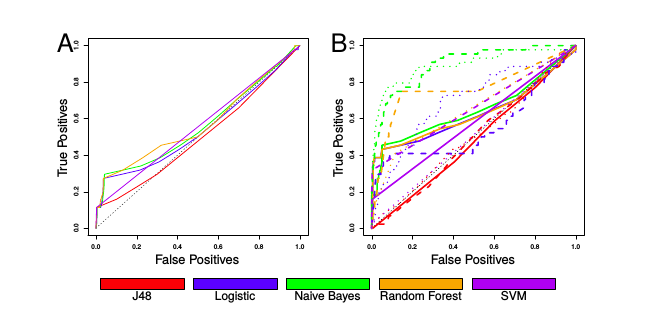
\includegraphics[width=.9\textwidth]{ROC_classification_seed.png}
  \caption{The ROC of classifiers that use hand chosen key words (a) and algorithmically chosen keywords (b) to determine if an individual is ill. The top 10 (solid line), 100 (dashed line), and 1000 (dotted line) were selected as features (taken from \citep{bodnar_ground_2014})}
  \label{fig:ROC_classification_seed}
  \end{figure}

% In a next step, the researchers turned to a manual semantic analysis of the 1609 tweets sent in a month in which their authors were sick with the flu as well as of 1609 control tweets sampled from the rest of the seed tweets. They found 58 tweets from 17 individual users which contained explicit expression of the author's disease status. 
% 
% contained any information about the users' disease status.

This model has its limitations as well, though: It was based on a very small data set consisting of only 104 twitter accounts generating a total of 37’599 tweets during the study period. Out of this sample, 35 users fell sick during the study period and generated a total of 1609 tweets in the month in which they were sick. Furthermore, all twitter users stemmed from the same state (Pennsylvania) and belonged to approximately the same socio-economic group (young students of the Pennsylvania State University). Hence, one would assume that their tweeting behaviour might be different from that of the average twitter use. In addition, the exact time of disease of the twitter users is not know. Due to privacy concerns, the researchers were limited to know in which month a specific twitter user was diagnosed with the flu. Finally, the model was built based on the tweeting behaviour and medical records of only one flu season (2011-2012). All these points either reduce the models' temporal resolution or add a considerable amount of bias to it. \newline

Hence, it is necessary to test the performance of the Naive Bayes classifier describe above for different cities and states and compare the results with reliable epidemiological data. In his dissertation \citep{bodnar_data_2015}, Todd Bodnar performed such tests on the level of counties, states, and the complete US mainland.\newline

To do so, he applied the classifier to the tweets of each user within a 4-week sliding window with a one-day step-size. ``The classifier assigns score (sic!) to the day where the sliding window begins based on the Tweets the user has posted within the window. For example, when the sliding window first encounters a user’s Tweet that says `I am getting sick with the flu', the classifier will heavily lean toward her being sick. Later, the user may Tweet `I am no longer sick' which will give a strong signal that the user is no longer sick which will tend to outweigh the user’s previous “sick” Tweet even if they both occur in the same window. Of course, it is rare that such strong signals are in the data, so the classifier is built on an amalgamation of many weaker signals—mentioning going to a party asnot-sick signal, for example—which, while weaker, are more prevalent. We chosestep size of one day in order to increase the temporal granularity of the classifier. Users that are inactive for more than 30 days are not included for any analysis during that time window."\footnote{Note that this way of assigning diseas status has one problematic implication, namely that information from future tweets is incorporated while information from past tweets are ignored. This insofar counterintuitive as a Twitter user who tweeted about being sick on day 1, will most certainly still be sick on day 2 - regardless of what she tweets about. However, the algortihm will not take into consideration any information from past days, so when shifting the onset of the 4-week-sliding window to day 2, all information from day 1 will be lost. If there are no additional flu keywords to be found in the tweets sent within the following 4-week-sliding window, the algorithm will mistakenly classify the user as being ``non sick". 
In addition, the algorithm is bound to classify tweets too early as being sick. For example, if particularly strong ``flu" signal turns up, the algorithm might classify the user as being ``sick" up to four weeks before the actual onset of the sickness. In other words; instead of assuming that a user remains sick for some time after she has tweeted about being sick, the algorithm might give the faulty impression that the user has been sick up to the point where she tweeted about it - but not afterwards.
There are no indications in the data set that something like this has happened, but since the overall number of users identified as being sick at any given point during the whole study time is very low, this does not mean much.}\newline

Bodnar applied the algorithm in the above-described fashion to a set of 15'560'328 users who sent a total of 2'732'174'105 geotagged tweets between March $3^\textit{rd}$ 2011 to March $4^\textit{th}$ 2015.\footnote{Note that tweets from users who tweeted less than 10 times during this period as well as tweets that could not be attributed to a specific state on the US mainland were discarded. However, the total number of tweets analysed was not given in any of the documentations available to me.} In a next step, Bodnar created a Kermack-McKendrick SIR model based on the results of the classifier \citep{martcheva2015introduction}:
$$\frac{dS}{dt} = -SI\beta, \qquad \frac{dI}{dt} = -SI\beta - I\gamma, \qquad \frac{dR}{dt} = I\gamma.$$
$S$, $I$, and $R$ represent the relative frequencies of susceptible, exposed, and recovered individuals, respectively, whereas $\beta$ and $\gamma$ are the transition probabilites from being susceptible to having the disease and from having the disease to recovering from it, respectively. To determine the values of $\beta$ and $\gamma$, Bodnar fitted the SIR model based on the data from the Twitter classifier to the official ILI results from the Center for Disease Control (CDC) in Atlanta using a multi-grid search method. Values for $\beta$ and $\gamma$ were chosen such that the corresponding SIR model minimised the residual sum of squares (RSS):
$$RSS = \sum_{t}(I_{\gamma,\beta}(t)-I_{CDC}(t)).$$
Here, $t$ denotes the time in weeks, while $I$ denotes the percentage of people showing ILI symptoms based on the SIR model ($$I_{\gamma,\beta}$$ and the official CDC data ($$I_{CDC}$$), respectively. By doing so, he calculated the optimal values of $\beta$ and $\gamma$ for each flu season as well as for the whole study period combined (see Table~\ref{tab:nationalparams}).\footnote{Note that in \citep{bodnar_data_2015} it is written that an optimal $S(0)$ was also estimated using the multi-grid search method. However, in the R-code provided to me $S(0)$ was simply defined as $1-I(0)$, where $I(0)$ is the relative number of Twitter users classified as ``sick" during the first week of the time window the SIR-model was built on.}

\begin{table}[H]
\centering
\begin{tabular}{l l l l l}

 Year & \(\gamma\) & \(\beta\) & RSS\\ \hline
& 0.1732 & 0.1749  & 0.0001047   \\ 
 {\multirow{-2}{*}{ 2011-2012 }}  & \cellcolor{grey}0.1176  & \cellcolor{grey}0.1195  & \cellcolor{grey}0.0001323  \\ \cline{2-4}
  {\multirow{2}{*}{ 2012-2013 }}& 0.7715 & 0.9626 & 0.0009402   \\ 
   & \cellcolor{grey}0.7317  & \cellcolor{grey}0.9020 & \cellcolor{grey}0.0009492   \\ \cline{2-4}
  {\multirow{2}{*}{ 2013-2014 }}& 0.6054 & 0.7288   & 0.0003114   \\ 
   & \cellcolor{grey}0.6046 & \cellcolor{grey}0.7264 & \cellcolor{grey}0.0003026  \\ \cline{2-4}
  {\multirow{2}{*}{ Combined }}& 0.6998 & 0.8225  & 0.003719   \\ 
   & \cellcolor{grey}0.6765  & \cellcolor{grey}0.7935  & \cellcolor{grey}0.003252   \\ 
\end{tabular}
\caption{National best-fit parameters for each year from the CDC's data (white) and Twitter data (grey); taken from \citep{bodnar_ground_2014}}
\label{tab:nationalparams}
\end{table}

Based on these values he could then calculate yearly ILI estimates for the flu seasons of 2011-2012, 2012-2013, and 2013-2014 (see Figure~\ref{fig:cdc_fit_bodnar_thesis_SIR})\newline

\begin{figure}[H]
  \centering
    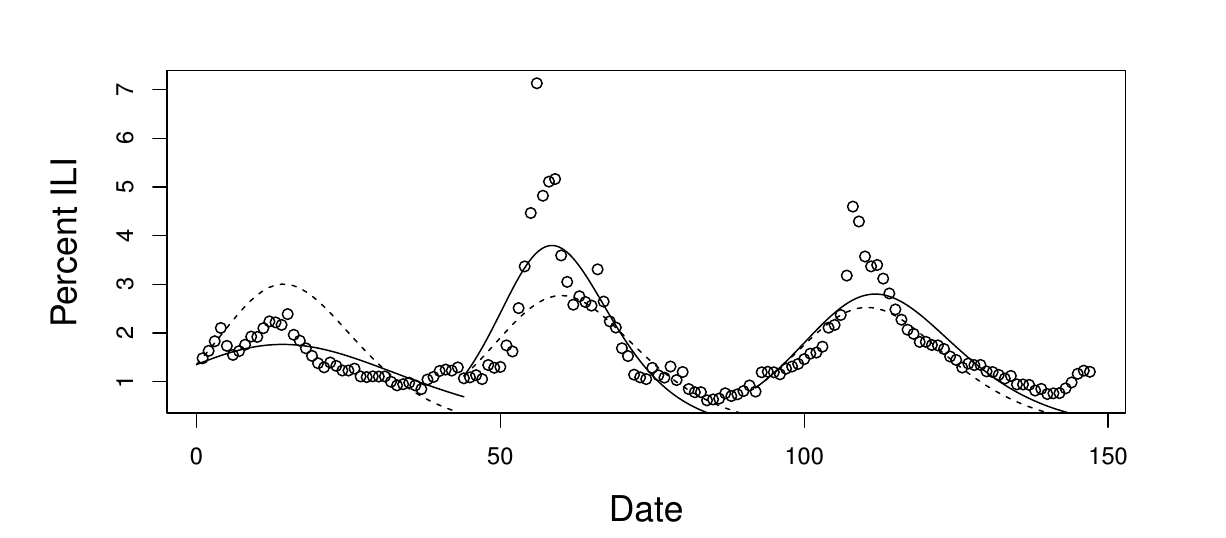
\includegraphics[width=.9\textwidth]{todd_bodnar_SIR.png}
  \caption{The CDC's estimates (circles) of influenza rates for a three year period compared to the best fit SIR models from the Twitter data using combined (dashed line) or yearly (solid line) parameters (taken from \citep{bodnar_data_2015})}
  \label{fig:cdc_fit_bodnar_thesis_SIR}
  \end{figure}

%This model served him to calculate $R_0$ \citep{heesterbeek2002brief}
In addition, he fitted a autocorrelation model using the results from the Twitter base model and dthe official CDC data: 

$$ILI(t+1) = a*I_{CDC}(t-1) + b*I_{CDC}(t) + c*I_{Twitter}(t)+d$$

Here, $t$ denotes the time in weeks, $I_{CDC}$ depicts the official ILI percentages from the CDC (lagged by two and one weeks, respectively), and $I_{Twitter}$ denotes the ILI percentages received from the Twitter base model. \footnote{Personal communication by Todd Bodnar. Note that it is unclear whether the ``Twitter base model" consists of the raw results from the Twitter classifier or consists of these raw results combined with additional information. An e-mail requesting clarification of this has been sent on June 24th, with three more follow-up emails sent in June and August. However, a clear description of how the Twitter base model was calculated is still missing. Also, I am still missing the values for $a$, $b$, and $c$, since I only received a file with the model results, but not the paramater specifications.}\newline

Applying the above-described autocorrelation model, Bodnar was able to achieve a very close fit to the official Twitter data (see Figure~\ref{fig:cdc_fit_bodnar_thesis}).This Master thesis is the (unsuccessful) attempt to reproduce these results. 

\begin{figure}[h]
  \centering
    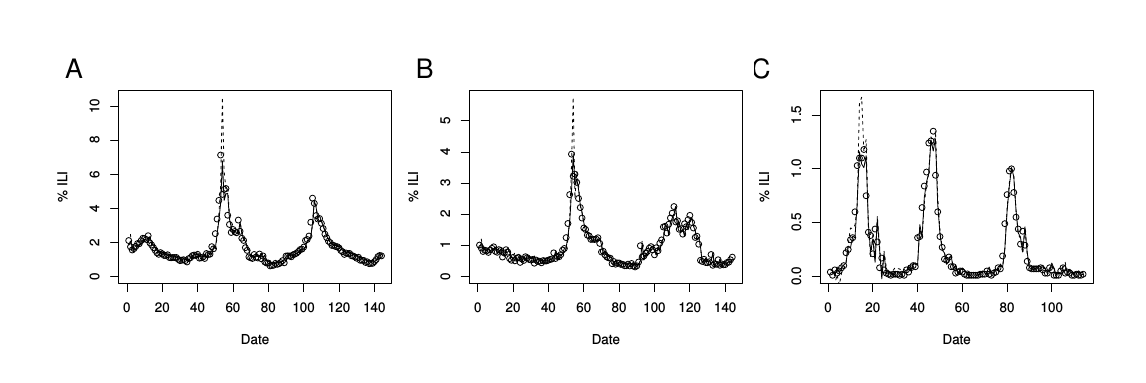
\includegraphics[width=.9\textwidth]{cdc_fit_bodnar_thesis.png}
  \caption{Comparison of Twitter's forecasting (dashed lines) and retroactive measurements (solid lines) to the CDC's reported Influneza rates (circles) for national (A), HHS Region 1 (B), and Seattle area (C) (taken from \citep{bodnar_data_2015})}
  \label{fig:cdc_fit_bodnar_thesis}
  \end{figure}

\chapter{Description of the data set}
\label{ch:data_set_description}
In the following I will describe the basic characteristics of the data set used. If not mentioned otherwise, all manipulations of the data set were done using \citeppackages{Rbase}. I will cite each package in addition to Rbase I used, but since single packages are used for several functions, I will only cite when they are mentioned the first time. All functions and data sets are available at xy.

\section{The starting point}

At the beginning of my analysis, I was handed a data set with tweet ratings, subdivided into three different sets: 

\begin{itemize}
  \item \textbf{all\_tweets} contains the whole set of rated tweets (\ensuremath{2.8470397\times 10^{9}} rows)
  \item \textbf{one\_hundred} contains the rated tweets of those users who sent at least 100 tweets (\ensuremath{4.2611004\times 10^{7}} rows)
  \item \textbf{sick} contains the rated tweets of all those users who sent at least one sick tweet (\ensuremath{4.13165\times 10^{6}} rows)
\end{itemize}

Each of the sets contains a row per tweet with the following six columns: 

\begin{knitrout}
\definecolor{shadecolor}{rgb}{0.969, 0.969, 0.969}\color{fgcolor}\begin{kframe}
\begin{verbatim}
##          userID longitude latitude       time sick state
## [1,] 1000007198 -86.34844 39.63168 1424580963    0    30
## [2,] 1000007198 -86.34844 39.63168 1424580963    0    30
## [3,] 1000009051 -87.63464 24.39631 1409880397    0    56
## [4,] 1000009051 -87.63464 24.39631 1409880397    0    56
## [5,] 1000010509 -90.14008 29.86666 1394405061    0    36
## [6,] 1000010509 -90.13791 29.88957 1411750890    0    36
\end{verbatim}
\end{kframe}
\end{knitrout}

\begin{itemize}
  \item \textbf{userID} a unique identifier of each Twitter user in the data set
  \item \textbf{longitude} geographical longitude in decimal degrees
  \item \textbf{latitude} geographical latitude in decimal degrees
  \item \textbf{time} UNIX timestamp marking the time when tweet was sent
  \item \textbf{sick} binary variable indicating whether tweet was labelled as ``sick=1" or ``healthy=0" by the Twitter rating algorithms
  \item \textbf{state} U.S. state (or District of Columbia) in which the tweet was sent
\end{itemize}

I ignored the \textit{one\_hundred} data set and only analysed the other two sets. All data sets were handled using \citeppackages{datatable} or \citeppackages{bigmemory}.

\section{Description of the \textit{sick} data set}
\label{sec:sick_user_exploratory}



As mentioned above, the \textit{sick\_user} data set should contain all tweets from those users who had at least one of their tweets labelled as ``sick" by the classifier.\newline

First, I preprocessed and filtered the data set in order to remove all those tweets that were sent from outside the US mainland (e.g. from the northern Mexico or southern Canada) or were otherwise incorrectly geolocated (e.g. having coordinates which locate the tweeter in the middle of the ocean). To do so, I excluded all tweets lying outside a rough rectangular window with W -125° to W -66° representing the longitudinal and N 25° to N 50° representing the latitudinal expansion of the window. This way, a total of 42860 entries were removed with 4088790 entries remaining.\newline

In the next step, I ran a custom-written function using a polygon lookup based on the coordinates of each tweet to determine the statename as well as to remove all those tweets which could not be assigned to any specific state. Of course, one might wonder why I did not just use the state code already present in the data set to assign each tweet to its respective state. There are two reasons for this: First, I did not have any reference table relating the state codes to the respective state names. Second, the polygon serves as an additionol control for the reliability of the data set. If state codes could not clearly be assigned to a specific state, this would mean that the codes could not be used as reference for future analyis. Luckily, this doesn't seem to be the case. Each state code could clearly be assigned to a specific US state with the sole exception of state code ``56", which comprised all those tweets that came to lie on a state or country border, were sent from Mexico or Canada, or were geolocated to the ocean (see Figure~\ref{fig:code56})\newline

Most of them came to lie either a the coastline or the Canadian-US-border and the Mexican-US-border, respectively. I removed a total of 180290 tweets that were sent from either Canada or Mexico (see Figure~\ref{fig:canexico_and_removed}). In order to reassign the unassigned tweets from the coastline, I first changed the coordinates of the ``border cases" by 0.1 degrees longitude and latitude towards the center of the US main land (e.g. if a tweet was sent from northeastern Canadian border, I added 0.1 degrees to its longitude and subtracted 0.1 degrees from its latitude before re-running the code). Those tweets that were still unassigned, received the same state name as majority of their neighbours within a 0.1x0.1 degree window. This way, a an additional 211511 tweets were removed, most of them at the coastline or from the ocean (see Figure~\ref{fig:canexico_and_removed}).\newline

\begin{figure}[h]
  \centering
    \begin{subfigure}[t]{0.9\textwidth}
    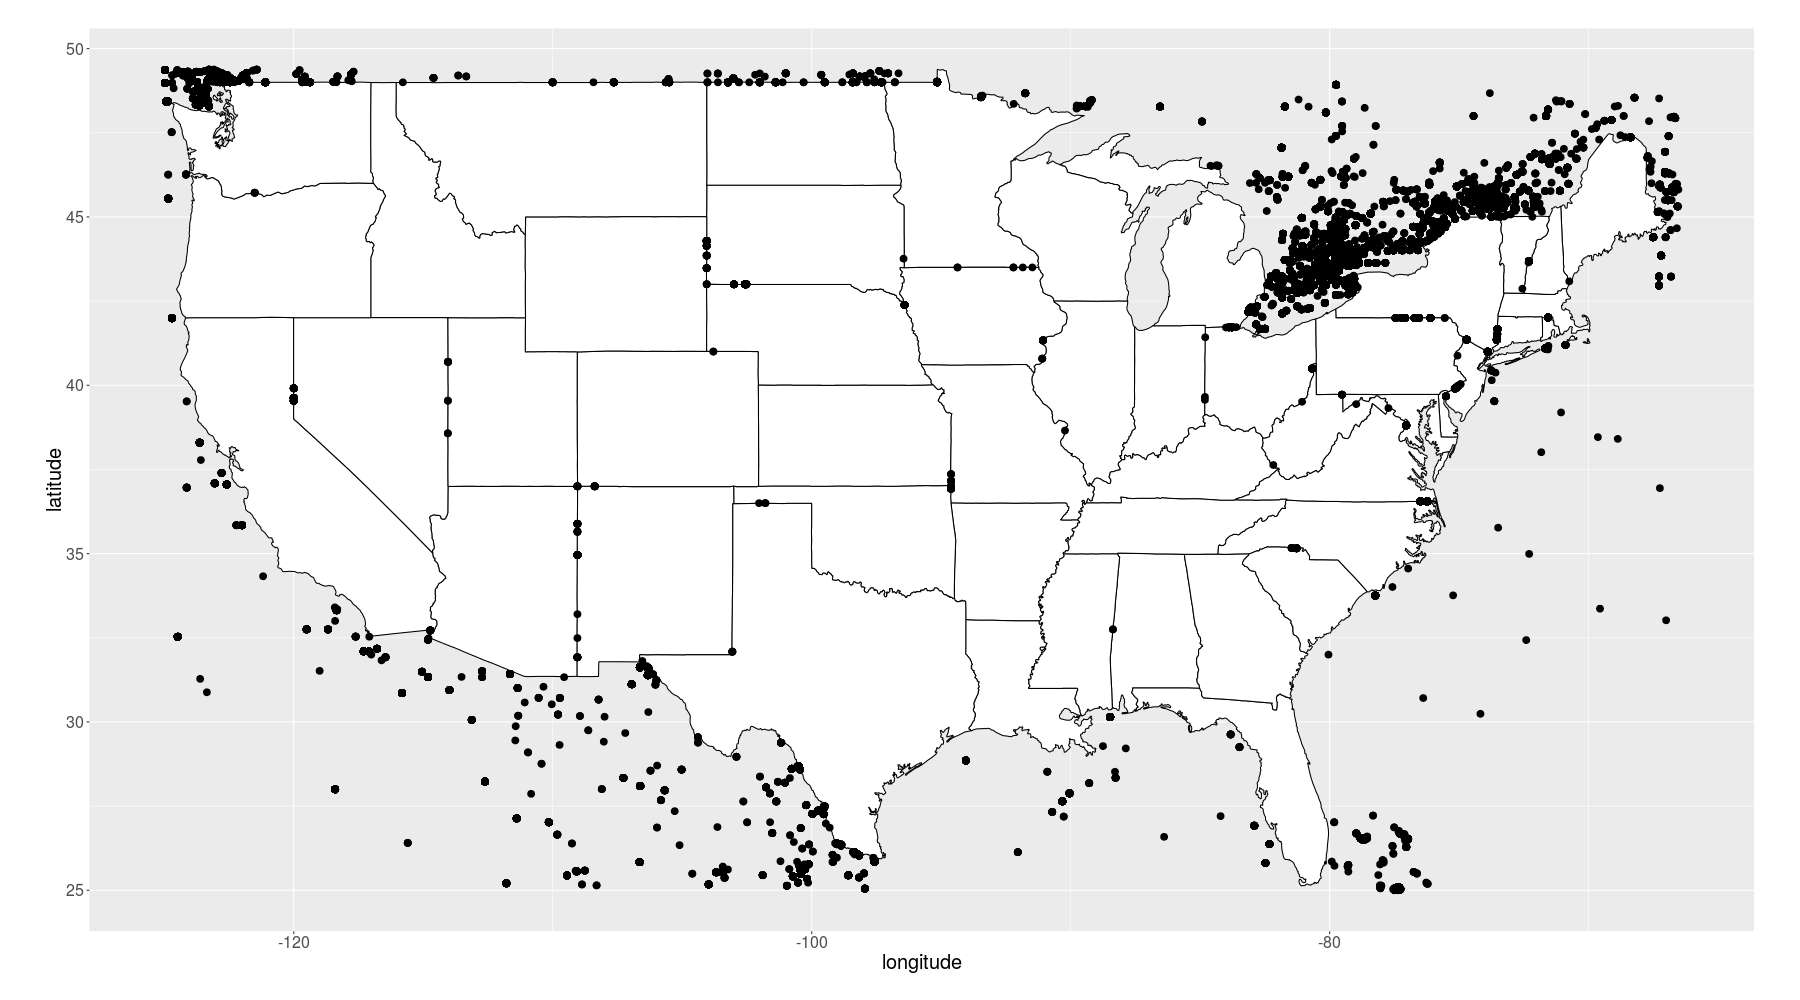
\includegraphics[width=1\linewidth]{state56_sick_raw_df.png}
    \caption{}
    \label{fig:code56}
  \end{subfigure}
  \begin{subfigure}[t]{0.9\textwidth}
  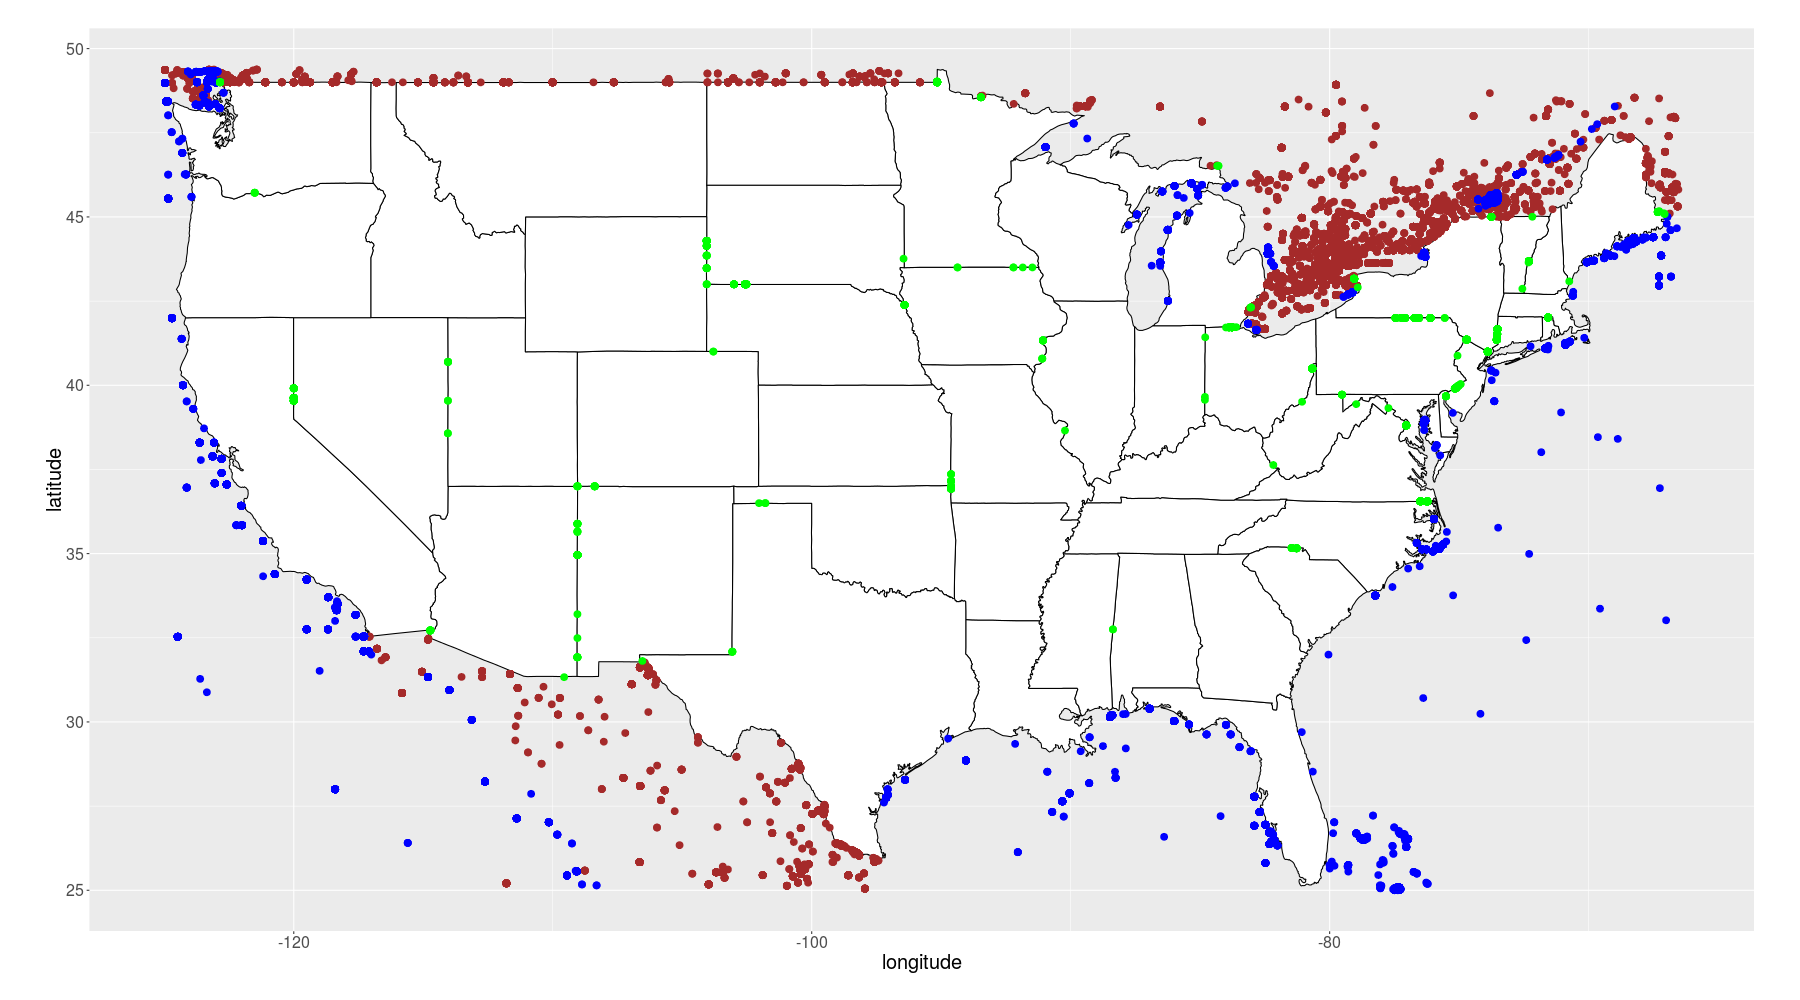
\includegraphics[width=1\linewidth]{CanexicoAndRemoved_sick_raw_df.png}
  \caption{}
  \label{fig:canexico_and_removed}
  \end{subfigure}
  \caption{(a) All tweets having ``state = 56" as code in the \textit{sick\_user} data set. These tweets could not be assigned to to any specific US state (b) Tweets whose origins was determined to be in Canada or Mexico (brown) or which could not be assigned to any US state (blue, mainly from the coastline or the ocean) and thus were removed from the \textit{sick\_user} data set. The green dots represent the tweets that had a ``state = 56" as  a code, i.e. that could not be assigned to any specific state in the original data set, but that could be recovered by the polygon lookup I performed. Note that the set of tweets shown in (b) is bigger than the set of tweets with state code ``56". This is because some tweets were removed that did \textbf{not} have state code ``56", but failed to be assigned to a state by the polygon lookup I performed.}
  \end{figure}

Afther pre-processing the \textit{sick\_user} data set was left with a with 3696989 tweets remaining. These tweets were sent by total of \ensuremath{2.13426\times 10^{5}}, meaning that on average, each user sent 17.3221116 tweets. This is in stark contrast to the number of tweets reported in \citep{bodnar_data_2015} (175.59 Tweets per user over the whole study period). A slight decrease in the average tweet number should be expected due to the fact that I discarded those tweets outside the designate time or geographical window. However, a tenfold decrease in average tweet number seems suspect (the time window analysed in \citep{bodnar_data_2015} was March 3rd 2011 to March 4th 2015, so only sligthly longer than in my case). Furthermore, the maximal number of tweets sent per user over the course of the 208 week period was 86, an incredibly low number given the fact that there twitter users out there who sent over a hundred tweets \textbf{per day} (see also Figure~\ref{fig:histogram_ID_tot}) for distribution of the number of tweets sent per user in the \textit{sick\_user} data set). Hence, I am led to believe that the \textit{sick\_user} data set does is not representative of rest of the data set, let alone the total corpus of tweets produced.\newline

\begin{figure}[h]
  \centering
    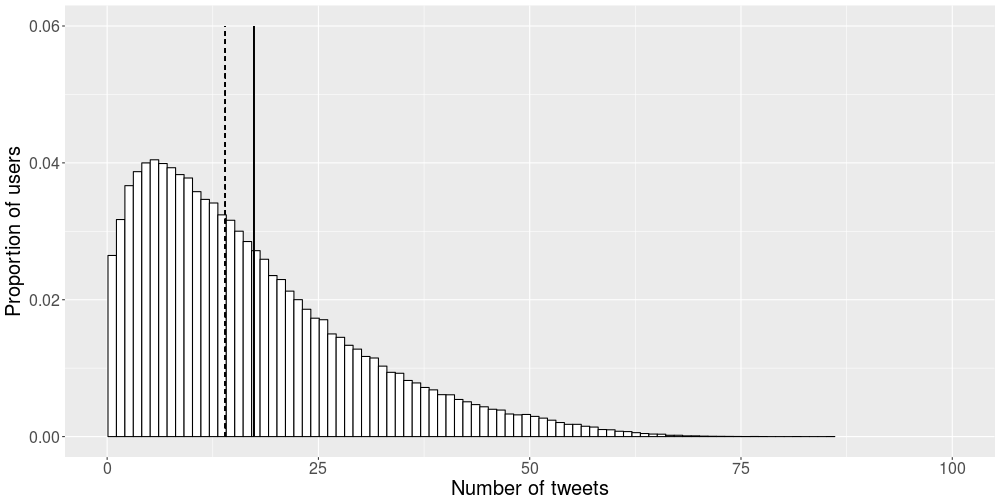
\includegraphics[width=1\textwidth]{user_activity_total_sick_raw_df.png}
  \caption{Histogram of the number of tweets sent per user in the \textit{sick\_user} data set during the 208 weeks between 2011-03-05 and 2015-07-11 (bin size = 1). As can be seen, many users only sent a handful of tweets during this time, whereas the user with the highest tweet activity sent 86 tweets. Mean = 17.3221116 (solid line); median = 14 (dashed line)}
  \label{fig:histogram_ID_tot}
\end{figure}

In addition, the large majority of the users within the \textit{sick\_user} data set never sent a tweet that was labelled as ``sick" by the flu classifier (see Figure~\ref{fig:barplot_sick_df}). In fact, only \ensuremath{2.0647\times 10^{4}} out of \ensuremath{2.13426\times 10^{5}} (or 9.6740791\%) ever sent such a tweet.\newline Also, a total of 919 users \textit{only} sent tweets that were labelled as sick - something that seems rather unlikely to happen. Finally, those \ensuremath{1.9728\times 10^{4}} users who sent both ``sick" and ``healthy" tweets had a significantly lower average tweet rate than those users who only sent ``healthy" tweets (16.0096817 and 17.5342179, respectively. p = \ensuremath{2.2723211\times 10^{-83}} using a Mann-Whitney U-Test). In fact, a Kolmogorov-Smirnov test indicates that the two subsets do not even follow the same probability distribution (p = 0), something that can also easily be seen in Figure~\ref{fig:both_vs_healthy_only_hist}.

\begin{figure}[h]
\centering
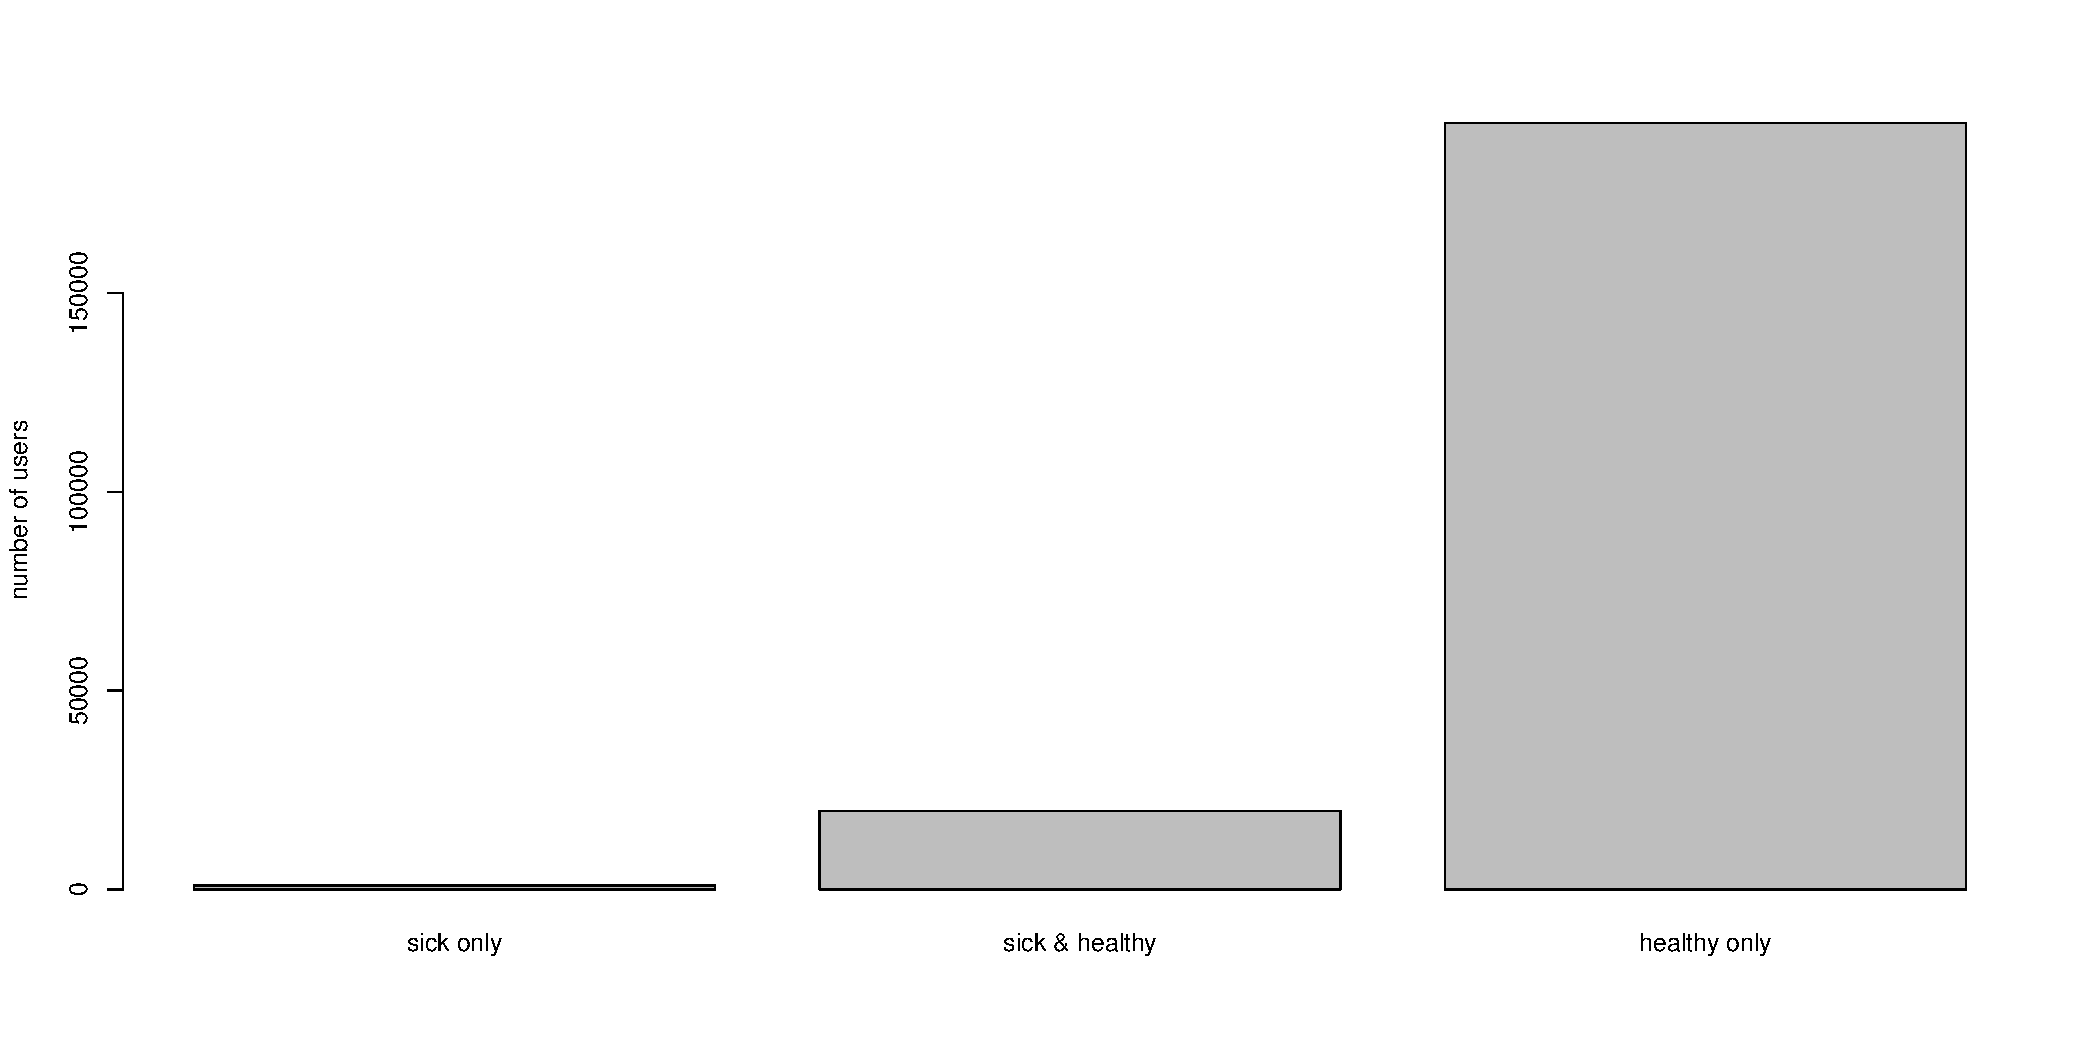
\includegraphics[width=1\linewidth]{barplot_sick_raw_df.pdf}
\caption{The total number of users who only sent tweets labelled as ``1 = sick" (919), users who sent at least one tweet labelled as ``1 = sick" and ``0 = healthy" (\ensuremath{1.9728\times 10^{4}}), and users who only sent tweets labelled as ``0 = healthy" (192779)}
\label{fig:barplot_sick_df}
\end{figure}

\begin{figure}[h]
\centering
  \begin{subfigure}[b]{1\textwidth}
  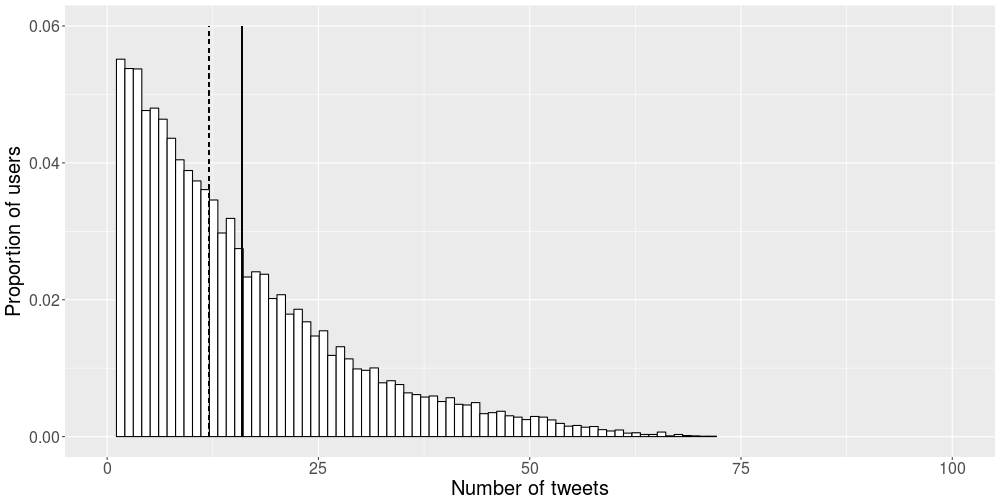
\includegraphics[width=1\linewidth]{user_activity_both_sick_raw_df.png}
  \caption{}
  \end{subfigure}
  \begin{subfigure}[b]{1\textwidth}
  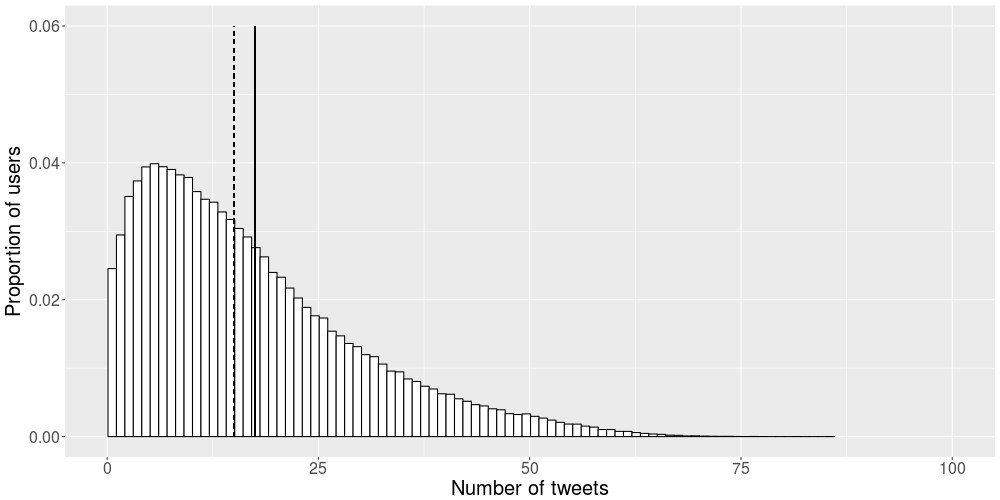
\includegraphics[width=1\linewidth]{user_activity_only_healthy_sick_raw_df.png}
  \caption{}
  \end{subfigure}
  \caption{Histogram of numbers of tweets sent per user during the 208 weeks between 2011-03-05 and 2015-07-11 (bin size = 1). (a) contains only tweets from users who sent at least one tweet labelled as ``1 = sick" and one tweet labelled as ``0 = healthy".  Mean = 16.0096817 (solid line); median = 12 (dashed line) (b) contains only tweets from users who never sent a tweet that was labelled as ``1 = sick" by the classifier.  Mean = 17.5342179 (solid line); median = 15 (dashed line). As can be seen, mode, median and mean of the number of tweets sent per user are significantly lower in (a) than in (b). Also, note that by construction (a) does not contain any user who only sent one tweet (since the users in this group are defined by having sent at last one tweet labelled ``1 = sick" and one tweet labelled ``0 = healthy")}
  \label{fig:both_vs_healthy_only_hist}

\end{figure}

Hence, it is unclear how exactly the \textit{sick\_user} data set was constructed, since it is neither a representative subset of the whole twitter data set (for that, the percentage for sick tweets is too high - see Section~\ref{sec:full_set}) nor does it exclusively contain tweets from users who had at least one of their tweets labelled as ``1 = sick".

Nevertheless, I used this data set as a basis to develop a basic grasp of the data set as well as to develop functions to analyse the data set in depth and to compare it with official flu data. However, I do not report any more results based on this data set, since the exact selection criteria used for this set are unclear and hence the inferences from it are not to be trusted. All following graphs, calculations and statistics are based on the full Twitter data set aggregated over weeks. 

\section{Description of the \textit{all\_tweets} data set}
\label{sec:full_set}

In order to analyse the complete data set with all \ensuremath{2.8470397\times 10^{9}}, I transformed them into ``big.matrix" objects using the \citeppackages{bigmatrix} package, removed all tweets before 2011-03-05 and after 2015-07-11 and aggregated the remaining \ensuremath{2.764211\times 10^{9}} tweets with regard to states and weeks in which the tweets where sent. The cut-off date for each week corresponded to the dates the official CDC flu reports were published. All tweets within the seven day time window leading up to a specific data were assigned to said date, including the tweets sent on that date (For example, if tweet was sent on 2015-07-11, 2015-07-07 or 2015-07-05 it was assigned to 2015-07-11. However, if it was sent on 2015-07-04 it was assigned to the previous week ending on 2015-07-10).\newline

Since there are a total a total of 208 weeks between 2011-03-05 and 2015-07-11 and a total of 50 different state labels in the original data set (48 labels for states on the US mainland, 1 label for the District of Columbia and 1 label for the tweets that could not be assigned to any of the former 49 areas), I received a data set with 10400 rows after aggregation (one for each state-week-pair). Each row has the following six columns:

\begin{knitrout}
\definecolor{shadecolor}{rgb}{0.969, 0.969, 0.969}\color{fgcolor}\begin{kframe}
\begin{verbatim}
##    week state sick  total healthy     sick_per
## 1:   23    34    1  86616   86615 1.154521e-05
## 2:  194    43    2  69629   69627 2.872366e-05
## 3:  155    16    0 140482  140482 0.000000e+00
## 4:   67    24  686 181757  181071 3.774270e-03
## 5:   40    28    0 101685  101685 0.000000e+00
## 6:   17     0    0  10142   10142 0.000000e+00
\end{verbatim}
\end{kframe}
\end{knitrout}

\begin{itemize}
  \item \textbf{week} the week in which the aggregated tweets were sent
  \item \textbf{state} the state in which the tweet were sent
  \item \textbf{sick} total number of tweets that were labelled as ``sick" in the given week and state
  \item \textbf{total} total number of tweets sent in the given week and state
  \item \textbf{healthy} total number of tweets that were not labelled as ``sick" in the given week and state
  \item \textbf{sick\_per} percentage of tweets labelled as sick among the total tweets sent in the given week and state
\end{itemize}


The complete data set consisted of a total of \ensuremath{2.8470397\times 10^{9}} tweets and hence was larger than the set reported by \citep{bodnar_data_2015} which contained 2,732,174,105 tweets. This difference is simply due to the fac the tweets in my data set were collecte until July 2015, while the tweets analysed in \citep{bodnar_data_2015} were only collected up to March 2015.\newline

In a first step, I removed all tweets before 2011-03-05 and after 2015-07-11 as well as outside the rough geographical window around the US mainland (W -125°, W -66°, N 25° , N 50° ) as described above, leaving \ensuremath{2.764211\times 10^{9}} tweets. \newline

Next, I added the corresponding date to each week index and then aggregated the whole data set with regard to week and state code (i.e. calculated the number of tweets sent within a given week in a given state). In order to assign state names to state labels present in the data set, I used the label/name relationships established in the \textit{sick\_user} data set (see section~\ref{sec:sick_user_exploratory}). Since tweets with state code ``56" predominantly stemmed from the Mexico and Canada or other areas outside the U.S. mainland (see Figure~\ref{fig:code56}), I removed all corresponding state/week pairs from the aggregated data set (\ensuremath{2.2335232\times 10^{8}} tweets in total), resulting in a data set with 10192 rows and 16 columns (see below), containing a total of \ensuremath{2.6147111\times 10^{9}} tweets aggregated over states and weeks.

\begin{knitrout}
\definecolor{shadecolor}{rgb}{0.969, 0.969, 0.969}\color{fgcolor}\begin{kframe}
\begin{verbatim}
##    week state sick  total healthy     sick_per            statename       date
## 1:   23    34    1  86616   86615 1.154521e-05            wisconsin 2011-08-13
## 2:  194    43    2  69629   69627 2.872366e-05             nebraska 2014-11-22
## 3:  155    16    0 140482  140482 0.000000e+00             delaware 2014-02-22
## 4:   67    24  686 181757  181071 3.774270e-03             kentucky 2012-06-16
## 5:   40    28    0 101685  101685 0.000000e+00            tennessee 2011-12-10
## 6:   17     0    0  10142   10142 0.000000e+00 district of columbia 2011-07-02
\end{verbatim}
\end{kframe}
\end{knitrout}

There were a total amount of \ensuremath{1.189809\times 10^{6}} tweets labelled as ``sick", a number that is considerably larger than the \ensuremath{2.0894\times 10^{4}} tweets labelled as ``sick" in the \textit{sick\_user} data set. This further shows that that the latter does not contain the full subset of tweets labelled as ``sick". Relatively speaking, 0.0455044 \% of all tweets in the \textit{all\_tweets} data set were labelled as ``sick" (as opposed to 9.6740791 \% in the \textit{sick\_user data set}).\newline

The total amount of users who have sent at least one tweet labelled as sick during the study period was \ensuremath{2.7052\times 10^{4}}. Not that this is an upper estimate, since a user could be classified as ``sick" more than once between 2011-03-05 and 2015-07-11. Since my analysis rests on weekly aggregated data, I would not be able to differentiate between a user who is classified as sick two times and two individual users who are classified as sick once. However, this is only a problem when assessing the total number of tweeters over the whole study period - it does not pose a problem when looking at the data categorised by weeks and/or states or at averaged data.\newline

What is peculiar, however, is the fact that the total number of sick users found in the twitter data set is considerably lower than the number reported in \citep{bodnar_data_2015} (182801 users labelled as> sick), despite the former being an upper estimate of the total number of individual sick users. At the other hand, the average number of individual users found in the data set during the first year (2011) for the whole country is \ensuremath{1.7538177\times 10^{5}}, while \citep{bodnar_data_2015} only reports a total of 45086 users being active during this year. Using the information that only around 0.85\% of all tweets are geotagged \citep{sloan_who_2015}, we can estimate the total number of Twitter users ative in 2011 based on the two mentioned sample estimates, respectively. While the former sample estimate gives us an average of \ensuremath{2.0633149\times 10^{7}} active users in 2011, the latter estimate based on \cite{bodnar_data_2015} only amounts to \ensuremath{5.3042353\times 10^{6}} total active users in 2011 - a number which is a far cry from the roughly 19 (March 2011) to 30 (December 2011) million of monthly active twitter users officially reported by Twitter in 2011 \citep{twitter_annual_2013}.\newline

In addition, I could observe a very peculiar difference in the average tweet frequency between healthy and sick users. While healthy users sent an average of 31.4178087 tweets per week, sick users sent an average 45.9534869 tweets per week (see Figure~\ref{fig:avg_tw_diff}), a difference that is highly significant (Mann-Whitney U-Test, p = \ensuremath{7.3631306\times 10^{-23}}). Also, the average tweet rate of all users combined (31.422503) is six times smaller than the average tweet rate per user reported in \citep{bodnar_data_2015} (175.59). The median (32.5294692) tweet rate, however, is considerably higher than the median tweet rate reported in \citep{bodnar_data_2015} (10).\newline

These points give reason to believe that the data used to build the ILI models reported in \citep{bodnar_data_2015} is not the same as the data I was analysing for this Master thesis.\newline

\begin{figure}[H]
\centering
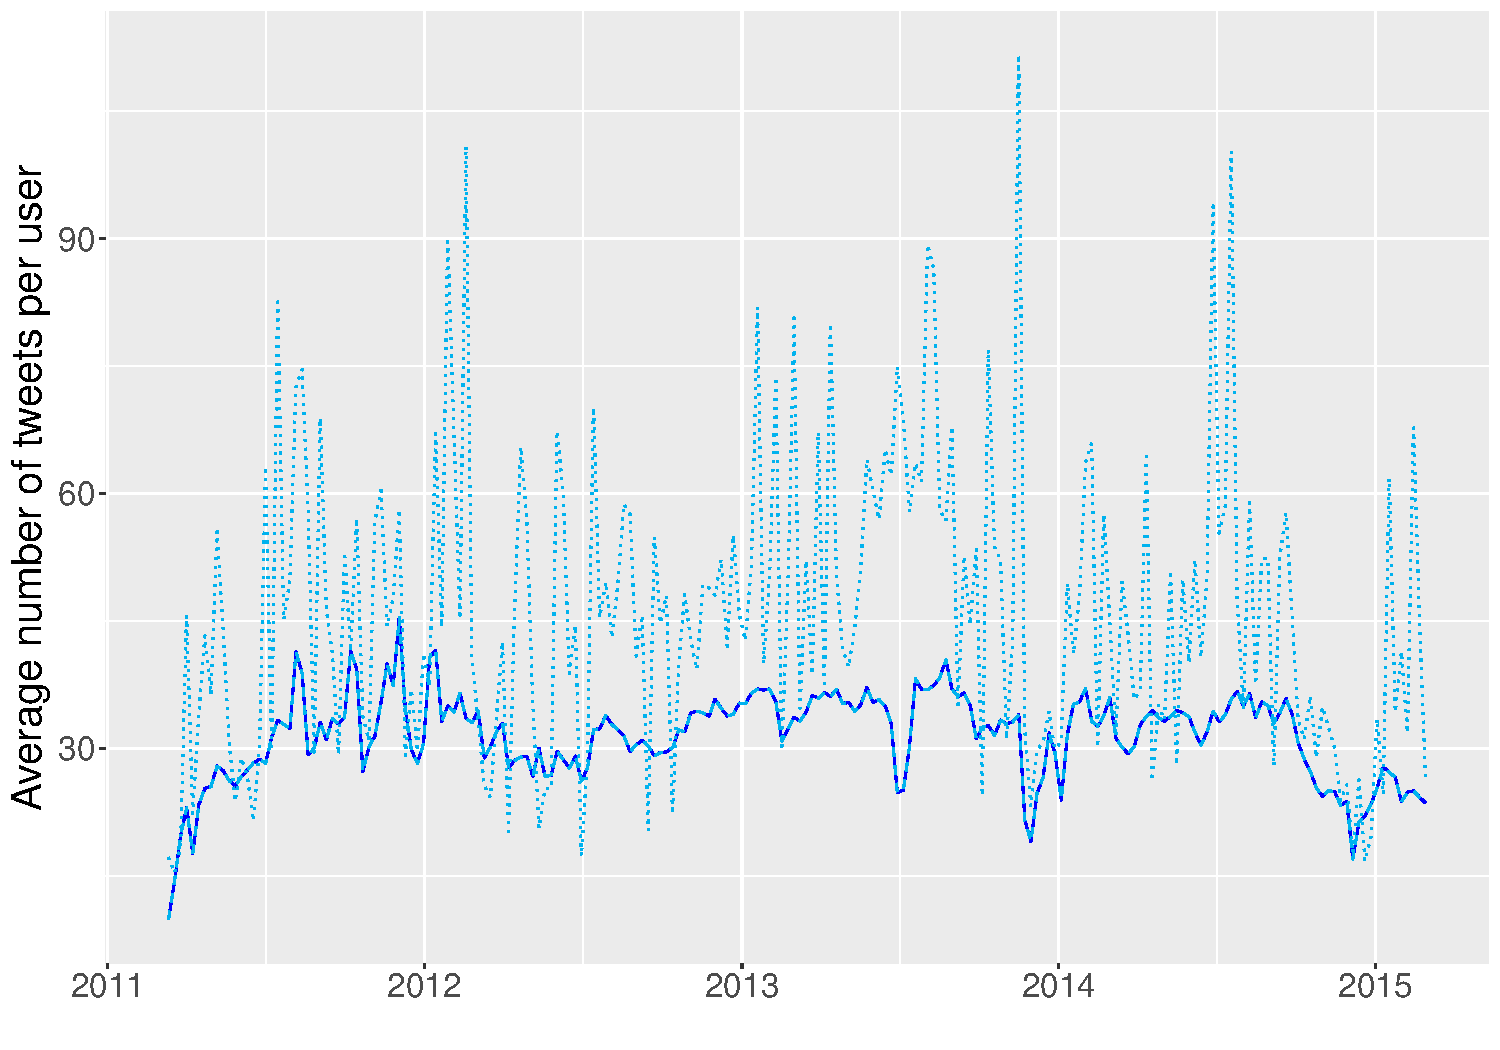
\includegraphics[width=1\linewidth]{avg_tw_sick_healthy.pdf}
\caption{The average number of tweets per week sent by sick users (dotted light blue), healthy user (dashed light blue) and total users (solid blue). The average weekly tweet rate of sick users is significantly higher, while the tweet rate of healthy users is virtually indistinguishable from the total weekly tweet rate.}
\label{fig:avg_tw_diff}
\end{figure}

\chapter{Results}
\label{ch:results}
Figure~\ref{fig:tweets_seasonal_full} shows the total number of tweets sent per week relative to the total number of tweets sent in the study period. here is no obvious pattern discernible other than an increase in weekly tweets until the third quarter of 2014 when a sudden dip in tweet activity occurs. The activity pattern of the tweets labelled as ``0 = healthy" is almost indiscernible from the temporal pattern of the complete data set. When looking at the weekly amount of tweets labelled as ``1 = sick" one can see a different pattern: The weekly activity is fluctuating more strongly and shows clearly discernible peaks towards the end and the beginning of each year. This pattern turns out to be even more pronounced when correcting for the total amount of tweets sent per week.\newline

A Kolmogorov-Smirnov test reveals that the weekly activity of the tweets labelled as ``1 = sick" is in fact significantly different from the weekly activity of the tweets labelled as ``0 = healthy" (p = 0.0264162 and p = 0 for the uncorrected and corrected weekly tweet counts). See Figure~\ref{fig:tweets_seasonal_healthy_sick} for a side-by-side comparison of both the uncorrected and corrected weekly tweet activity.\newline

\begin{figure}[H]
\centering
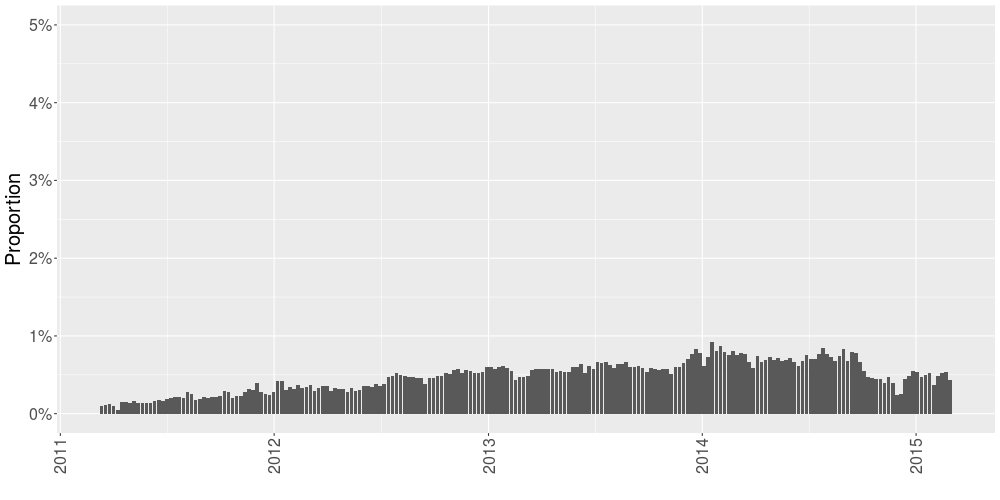
\includegraphics[width=1\linewidth]{activity_total_date_Twitter_full_aggregated.png}
\caption{Relative number of tweets sent per week in the \textit{all\_tweets} data set between 2011-03-05 and 2015-07-11 (bin size = 1 week).}
\label{fig:tweets_seasonal_full}
\end{figure}

\begin{figure}[H]
\centering
  \begin{subfigure}[t]{0.49\textwidth}
  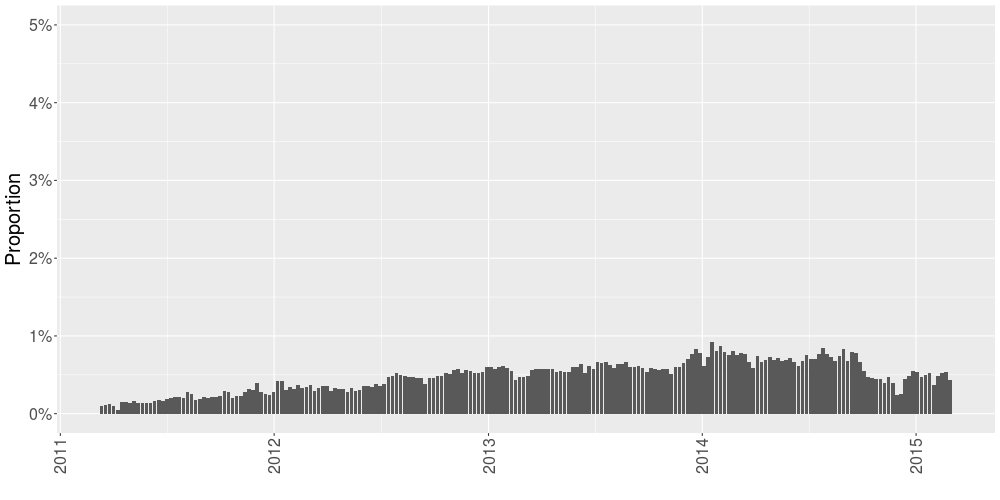
\includegraphics[width=1\linewidth]{activity_healthy_date_Twitter_full_aggregated.png}
  \caption{}
  \end{subfigure}
\hfill
  \begin{subfigure}[t]{0.49\textwidth}
  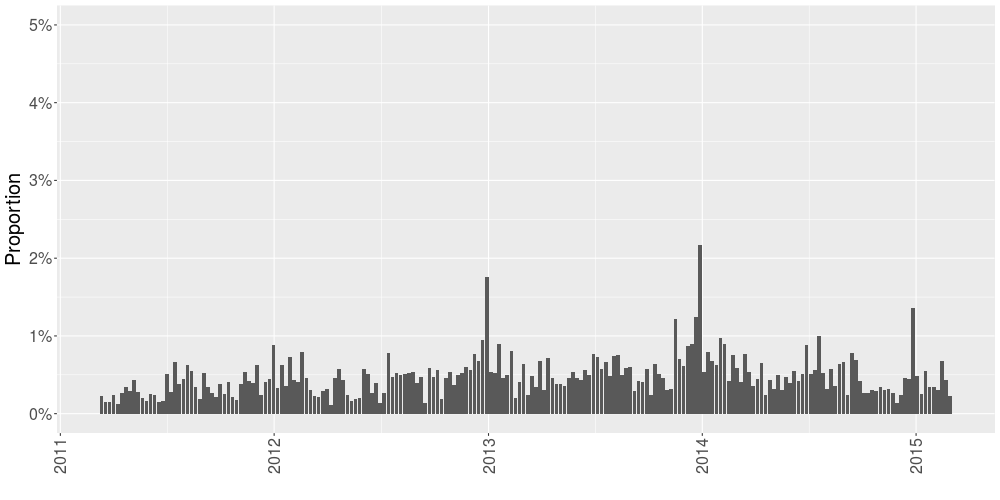
\includegraphics[width=1\linewidth]{activity_sick_date_Twitter_full_aggregated.png}
  \caption{}
  \end{subfigure}
  
  \bigskip 

    \begin{subfigure}[t]{0.49\textwidth}
  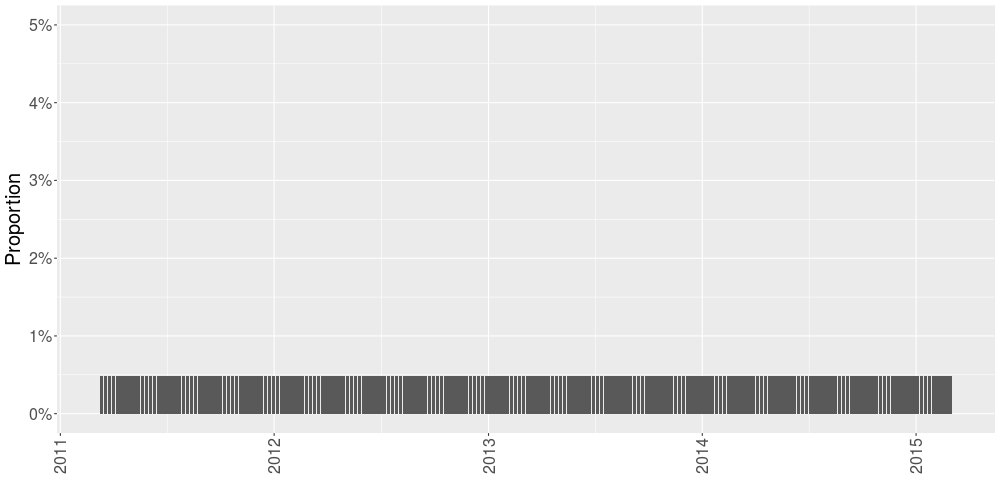
\includegraphics[width=1\linewidth]{activity_rel_healthy_date_Twitter_full_aggregated.png}
  \caption{}
  \end{subfigure}
  \hfill
    \begin{subfigure}[t]{0.49\textwidth}
  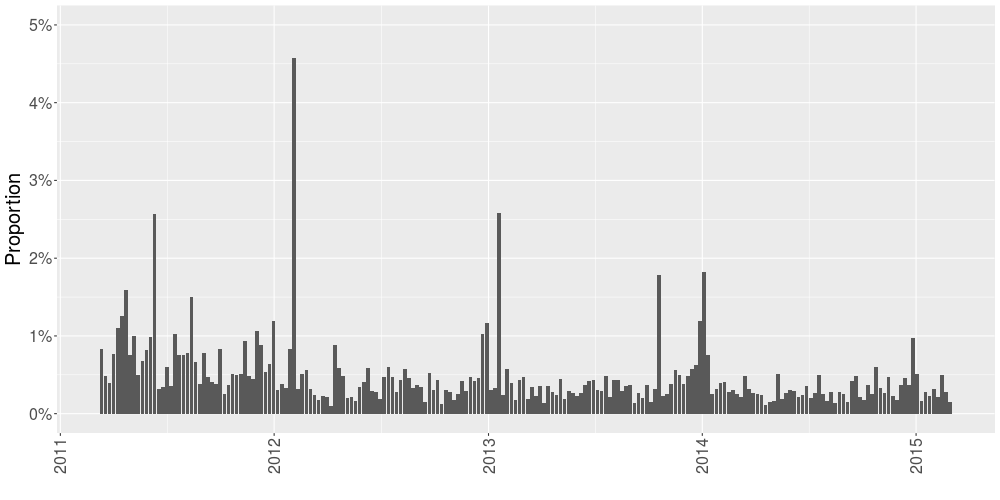
\includegraphics[width=1\linewidth]{activity_rel_sick_date_Twitter_full_aggregated.png}
  \caption{}
  \end{subfigure}
  \caption{Histograms of numbers of the tweets sent per week during the 208 weeks between 2011-03-05 and 2015-07-11 (bin size = 1 week). (a) and (c) contain only tweets labelled as ``0 = healthy"; (b) and (d) contain only tweets labelled as ``1 = sick" by the classifier. The lower two histograms were normalised by the total amount of tweets sent per week. As can be seen, the tweets labelled as ``1 = sick" follow a markedly different temporal pattern.}
  \label{fig:tweets_seasonal_healthy_sick}
\end{figure}

Next, I looked at the total amount of tweets sent in each state. As can be seen in Figure~\ref{fig:tweets_state_full} and in Figure~\ref{fig:tweets_state_full_scatter}, the relative distribution per state largely follows the relative distribution of the state population. Notable exceptions are Maryland and New Jersey, which were the origin of many more tweets than expected, as well as New York, from where considerably fewer tweets originated than would be expected with regard to its population.\newline

When comparing the relative number of tweets labelled as ``0 = healthy" with those labelled as ``1 = sick", we can see slight differences in the distribution, which become even more accentuated when normalising with the total number of tweets per state (Figure~\ref{fig:tweets_state_healthy_sick}) However, the states with the most pronounced differences (District of Columbia, Montana, South Dakotam, North Carolina) are almost all states or districts, respectively, with a very low overall tweet count (North Carolina being the exception). A Chi-Squared Test for independence between the two distributions gives a p-value of 0.0800653. Repeating the calculations using number of Twitter users instead of number tweets yields similar results (Figure~\ref{fig:tweets_state_full_user}, Figure~\ref{fig:tweets_state_full_scatter_user}, Figure~\ref{fig:tweets_state_healthy_sick_user}; p = 0.0822911)

\begin{figure}[H]
\centering
\begin{subfigure}[t]{1\textwidth}
  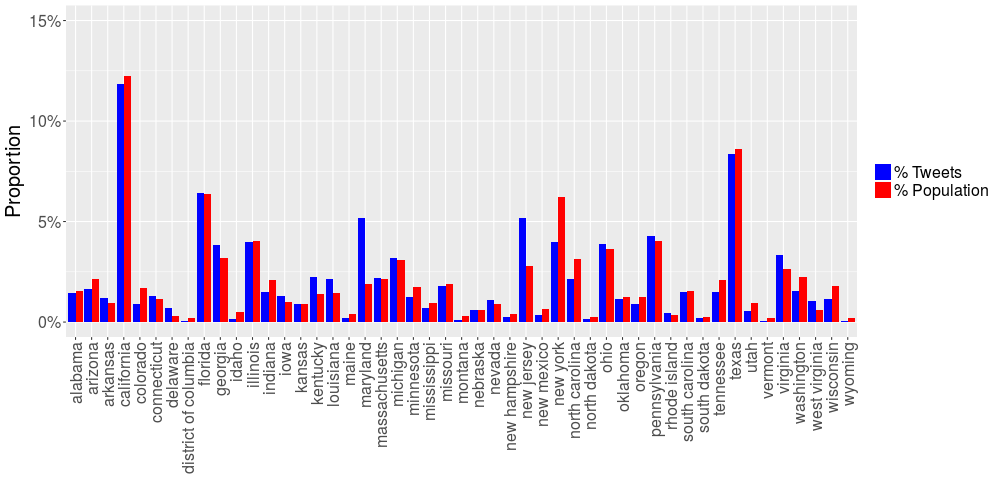
\includegraphics[width=1\linewidth]{activity_total_state_Twitter_full_aggregated.png}
  \caption{}
  \label{fig:tweets_state_full}
  \end{subfigure}
  
  \begin{subfigure}[t]{1\textwidth}
  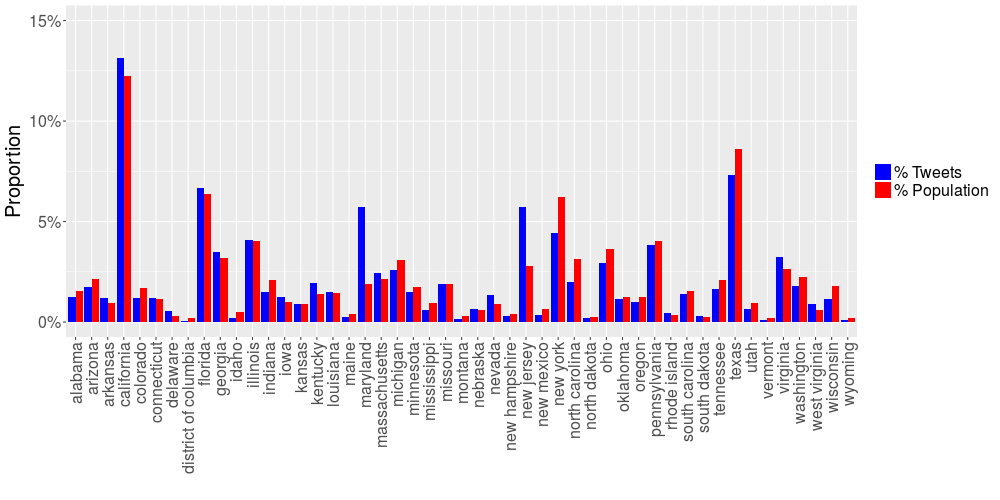
\includegraphics[width=1\linewidth]{activity_total_user_state_Twitter_full_aggregated.png}
  \caption{}
    \label{fig:tweets_state_full_user}
  \end{subfigure}
\caption{Relative number of tweets sent (a) and Twitter users (b) per state in the \textit{all\_tweets} data set between 2011-03-05 and 2015-07-11 compared to each state's relative population size.}
\end{figure}

\begin{figure}[H]
\centering
 \begin{subfigure}[t]{0.6\textwidth}
  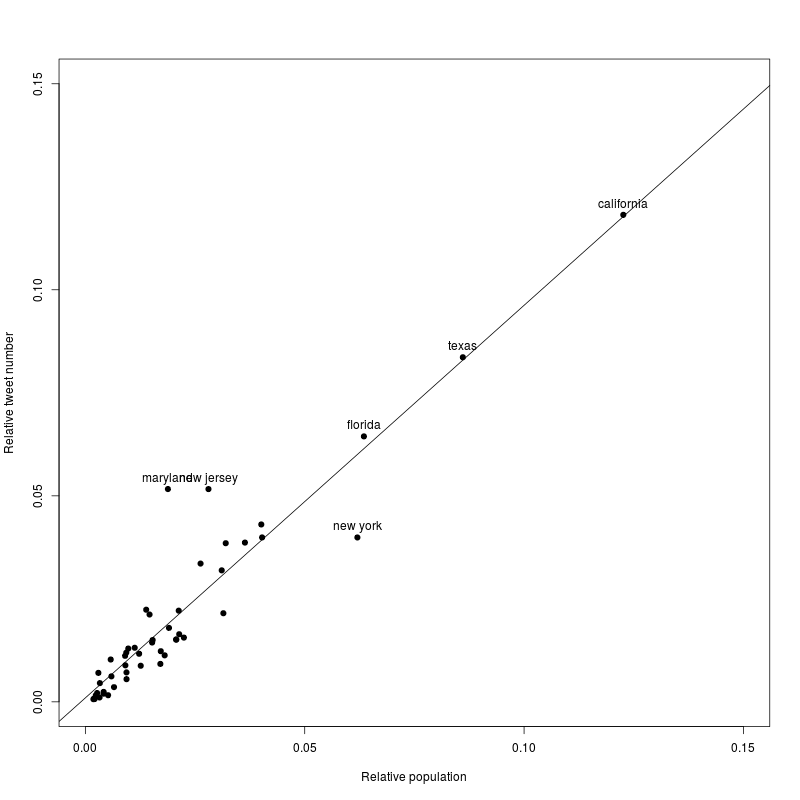
\includegraphics[width=1\linewidth]{ScatterTweetPop.png}
  \caption{}
  \label{fig:tweets_state_full_scatter}
  \end{subfigure}
  
  \begin{subfigure}[t]{0.6\textwidth}
  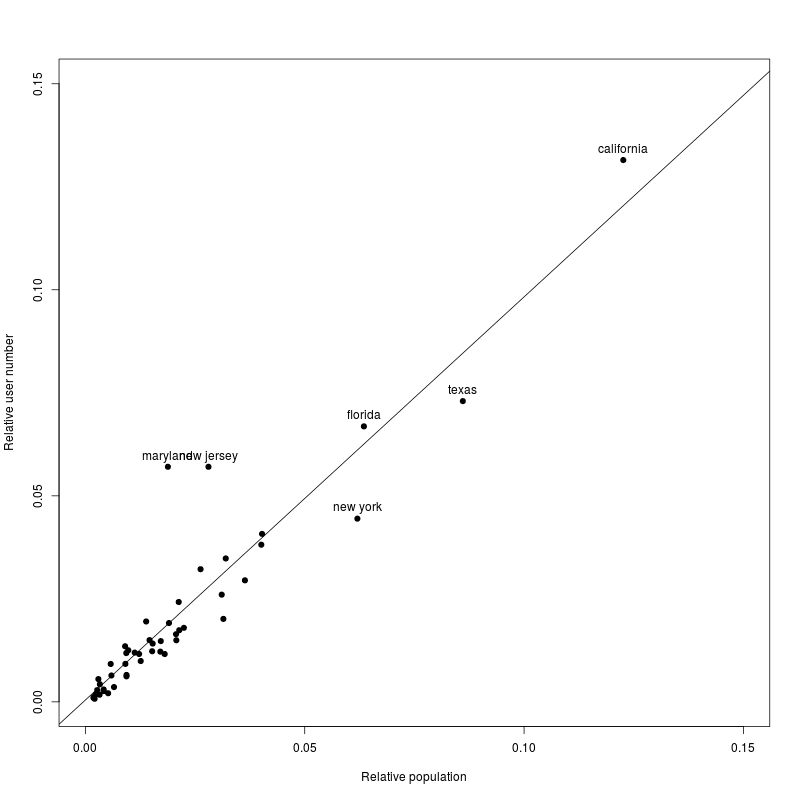
\includegraphics[width=1\linewidth]{ScatterTweetPop_user.png}
  \caption{}
  \label{fig:tweets_state_full_scatter_user}
  \end{subfigure}

\caption{Relative number of tweets sent per state (a) and Twitter users (b) in the \textit{all\_tweets} data set between 2011-03-05 and 2015-07-11 plotted against each state's relative population size}
\end{figure}

\begin{figure}[H]
\centering
  \begin{subfigure}[t]{0.49\textwidth}
  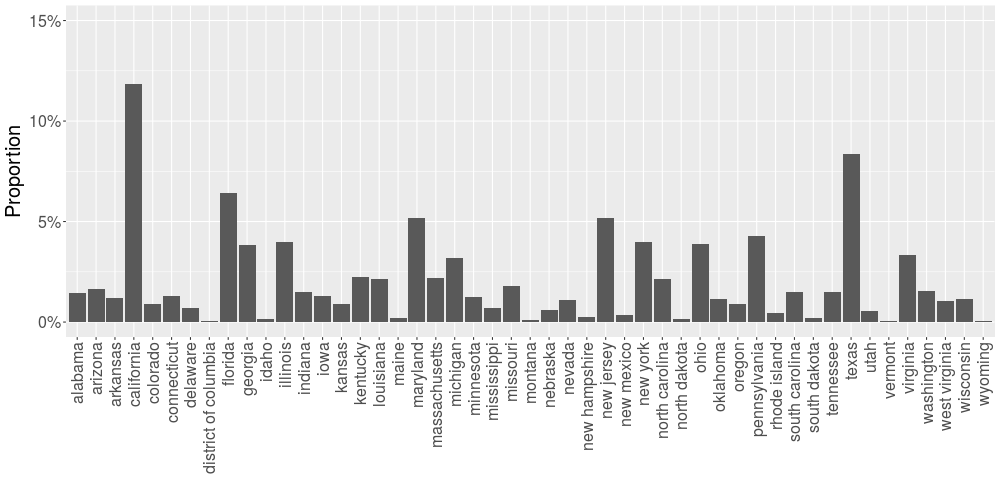
\includegraphics[width=1\linewidth]{activity_healthy_statename_Twitter_full_aggregated.png}
  \caption{}
  \end{subfigure}
\hfill
  \begin{subfigure}[t]{0.49\textwidth}
  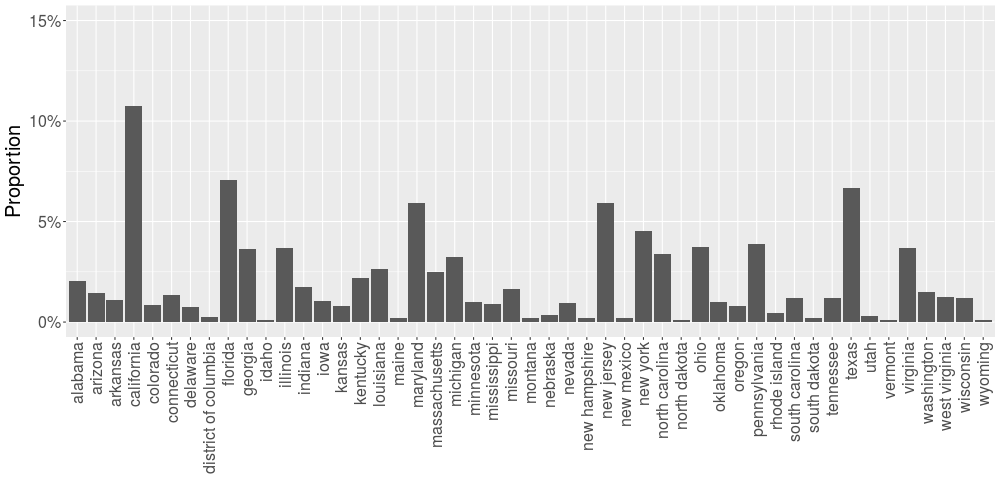
\includegraphics[width=1\linewidth]{activity_sick_statename_Twitter_full_aggregated.png}
  \caption{}
  \end{subfigure}
  
  \bigskip 

    \begin{subfigure}[t]{0.49\textwidth}
  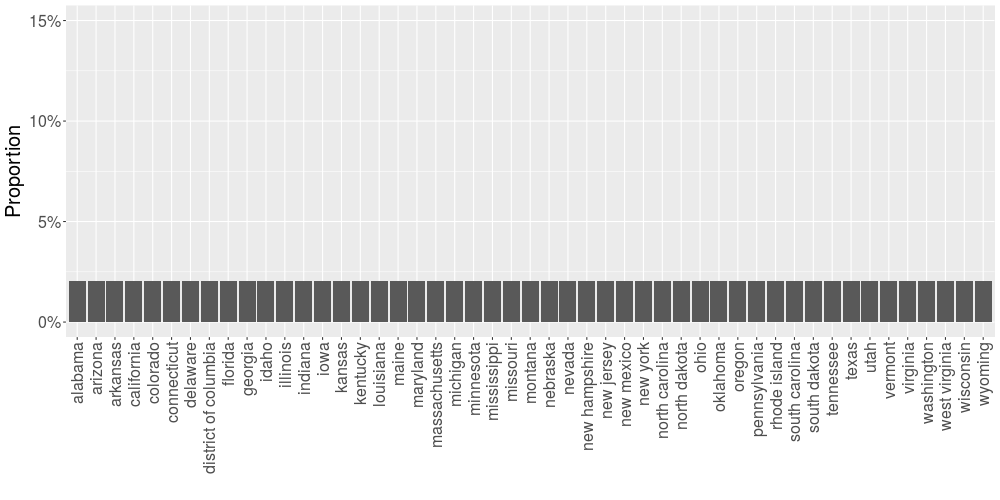
\includegraphics[width=1\linewidth]{activity_rel_healthy_statename_Twitter_full_aggregated.png}
  \caption{}
  \end{subfigure}
  \hfill
    \begin{subfigure}[t]{0.49\textwidth}
  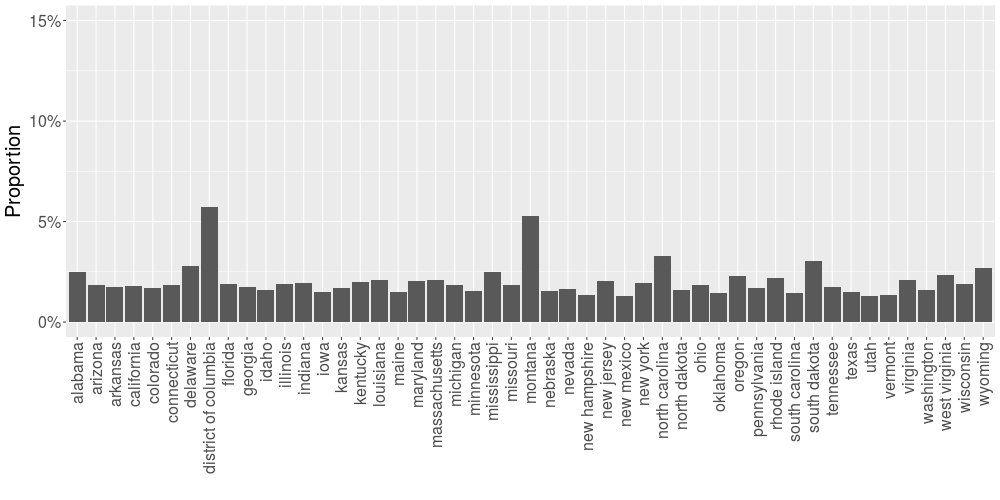
\includegraphics[width=1\linewidth]{activity_rel_sick_statename_Twitter_full_aggregated.png}
  \caption{}
  \end{subfigure}
  \caption{Histograms of numbers of the tweets sent in each state during the 208 weeks between 2011-03-05 and 2015-07-11 (bin size = 1 week). (a) and (c) contain only tweets labelled as ``0 = healthy"; (b) and (d) contain only tweets labelled as ``1 = sick" by the classifier. The lower two histograms were normalised by the total amount of tweets sent per state As can be seen, the tweets labelled as ``1 = sick" follow a somewhat different spatial pattern.}
  \label{fig:tweets_state_healthy_sick}
\end{figure}

\begin{figure}[H]
\centering
  \begin{subfigure}[t]{0.49\textwidth}
  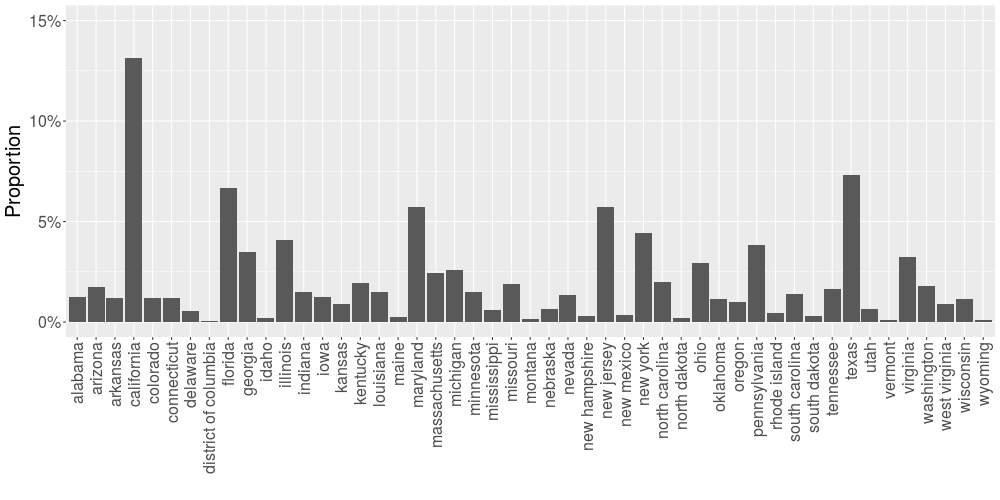
\includegraphics[width=1\linewidth]{activity_healthy_user_statename_Twitter_full_aggregated.png}
  \caption{}
  \end{subfigure}
\hfill
  \begin{subfigure}[t]{0.49\textwidth}
  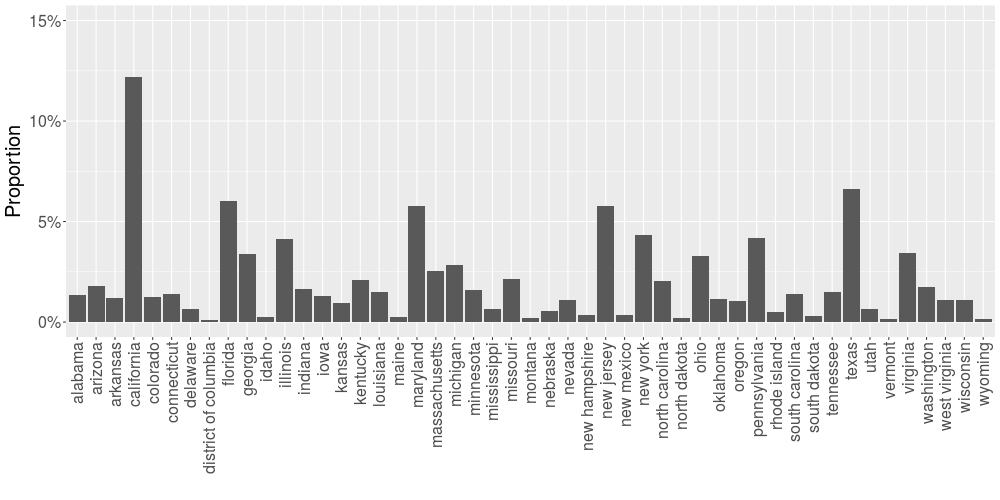
\includegraphics[width=1\linewidth]{activity_sick_user_statename_Twitter_full_aggregated.png}
  \caption{}
  \end{subfigure}
  
  \bigskip 

    \begin{subfigure}[t]{0.49\textwidth}
  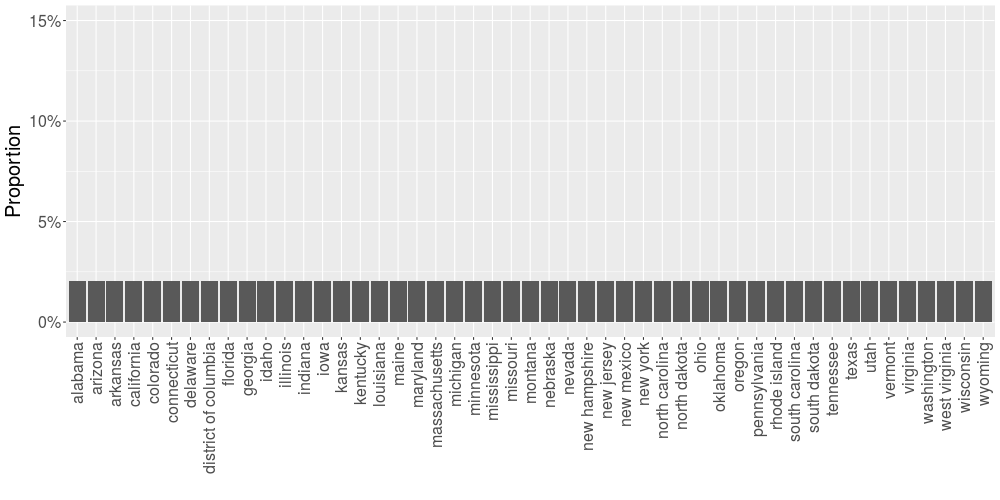
\includegraphics[width=1\linewidth]{activity_rel_healthy_user_statename_Twitter_full_aggregated.png}
  \caption{}
  \end{subfigure}
  \hfill
    \begin{subfigure}[t]{0.49\textwidth}
  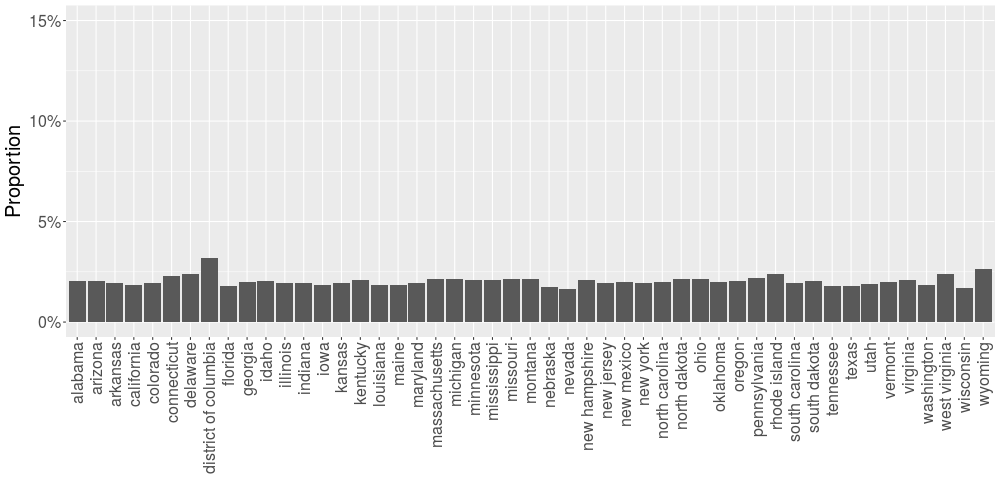
\includegraphics[width=1\linewidth]{activity_rel_sick_user_statename_Twitter_full_aggregated.png}
  \caption{}
  \end{subfigure}
  \caption{Histograms of number of users active in each state during the 208 weeks between 2011-03-05 and 2015-07-11 (bin size = 1 week). (a) and (c) contain only tweets labelled as ``0 = healthy"; (b) and (d) contain only users with at least one tweet labelled as ``1 = sick" by the classifier. The lower two histograms were normalised by the total number of user active per state. As can be seen, the users who were ``diagnosed" as ``sick" at some point by the classifier, follow almost the same spatial pattern.}
  \label{fig:tweets_state_healthy_sick_user}
\end{figure}

\section{Comparison with CDC data}
\label{sec:comp_cdc}

In order to assess the validity of the ILI predictions provided by the flu classifier, I compared the the results from the Twitter classifier with the official ILI reports from the CDC on the national, regional and state level(extracted using the ``cdcfluview" package \citeppackages{cdcfluview}).\newline

In a first step, I simply compared the official CDC ILI percentage data on the national level with the the relative number of tweets labelled as ``1 = sick" per week and the relative number of sick users per week, respectively. As can be seen from Figure~\ref{fig:naive_comparison_CDC_twitter}, the relative results from the Twitter classifer are an order of magnitude smaller than the official CDC data.

\begin{figure}[H]
\centering
  \begin{subfigure}[t]{0.49\textwidth}
  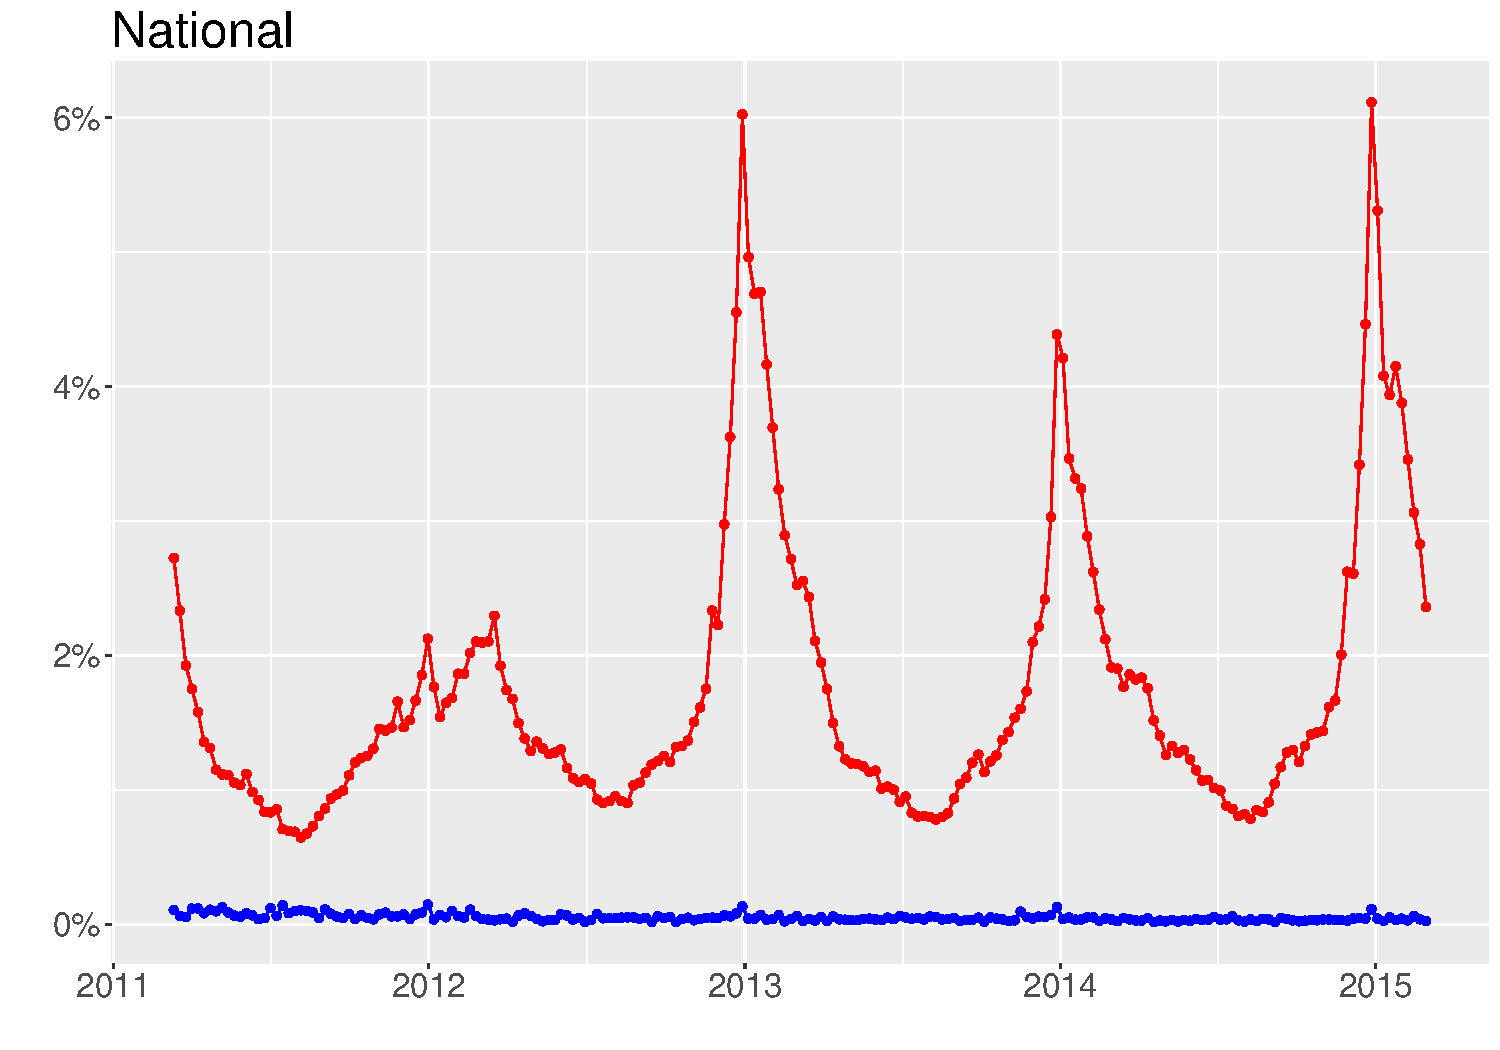
\includegraphics[width=1\linewidth]{cdc_twitter_comp_nat_raw.pdf}
  \caption{}
  \end{subfigure}
\hfill
  \begin{subfigure}[t]{0.49\textwidth}
  
\includegraphics[width=1\linewidth]{cdc_twitter_comp_nat_raw_user.pdf}
  \caption{}
  \end{subfigure}
  \caption{Comparison between weekly CDC ILI rates (red) and the results from the Twitter classifier (blue). (a) shows the relative amount of tweets labelled as sick during a given week. (b) shows the relative amount of users labelled as ``sick" by the classifier. As can be seen from both figures, the relative results from the Twitter classifer are an order of magnitude smaller than the official CDC data}
  \label{fig:naive_comparison_CDC_twitter}
\end{figure}

In order to make them directly comparable to each other, I normalised both time series by the total sum of relative tweets numbers and ILI percentages, respectively. Hence, the percentual values shown in Figure~\ref{fig:cdc_tw_comp_nat_ma1} do \textbf{not} represent weekly ILI percentage, but rather the percentual proportion of the relative number of tweets and the ILI percentages, respectively, of a given week within the whole 208 week study period (In other words: The percentages of each week add up to a 100\%). Since the fluctuations in the Twitter data were very high, I plotted the data again after applying a two-week (Figure~\ref{fig:cdc_tw_comp_nat_ma2}) and four-week (Figure~\ref{fig:cdc_tw_comp_nat_ma4}) moving average smoother (using the ``forecast" package \citeppackages{forecast}). This reduced the overall fluctuations a bit, but did not particularly improve the fit with the CDC curve. I did the same for each of the ten CDC flu surveillance regions (Figure~\ref{fig:cdc_tw_comp_regs_ma4}). The situation improves slightly if we use the relative amount of sick \textbf{users} per week (as opposed to the relative amount of sick \textbf{tweets} per week), as can be seen  from Figures~\ref{fig:cdc_tw_comp_nat_user} and \ref{fig:cdc_tw_comp_regs_ma4}. In both cases, however, the correlation between the relative ILI estimates based on Twitter data and the official CDC data were abysmal (Spearman's Rho was 0.0077319 and 0.0077319 for tweet- and user-based four-week average curves, respectively).\newline 

\begin{figure}[H]
\centering
  \begin{subfigure}[t]{0.6\textwidth}
  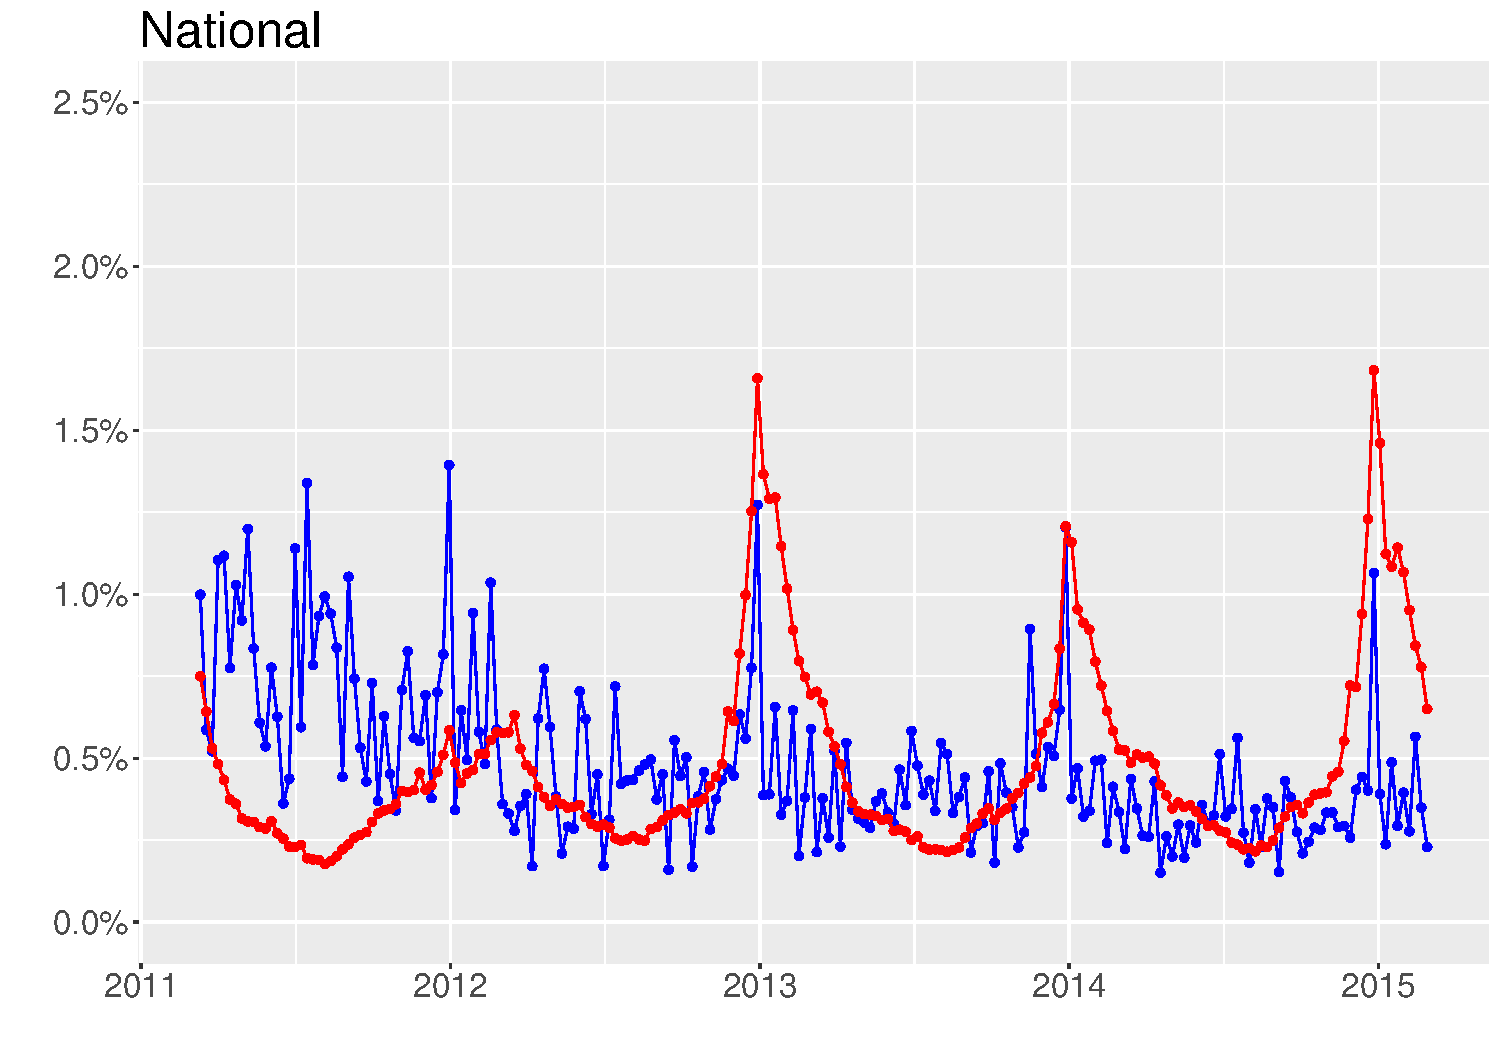
\includegraphics[width=1\linewidth,height=0.5\linewidth]{cdc_twitter_comp_nat_ma1.pdf}
  \caption{}
  \label{fig:cdc_tw_comp_nat_ma1}
  \end{subfigure}
  
  \begin{subfigure}[t]{0.6\textwidth}
  \includegraphics[width=1\linewidth,height=0.5\linewidth]{cdc_twitter_comp_nat_ma2.pdf}
  \caption{}
  \label{fig:cdc_tw_comp_nat_ma2}
  \end{subfigure}
  
  \begin{subfigure}[t]{0.6\textwidth}
  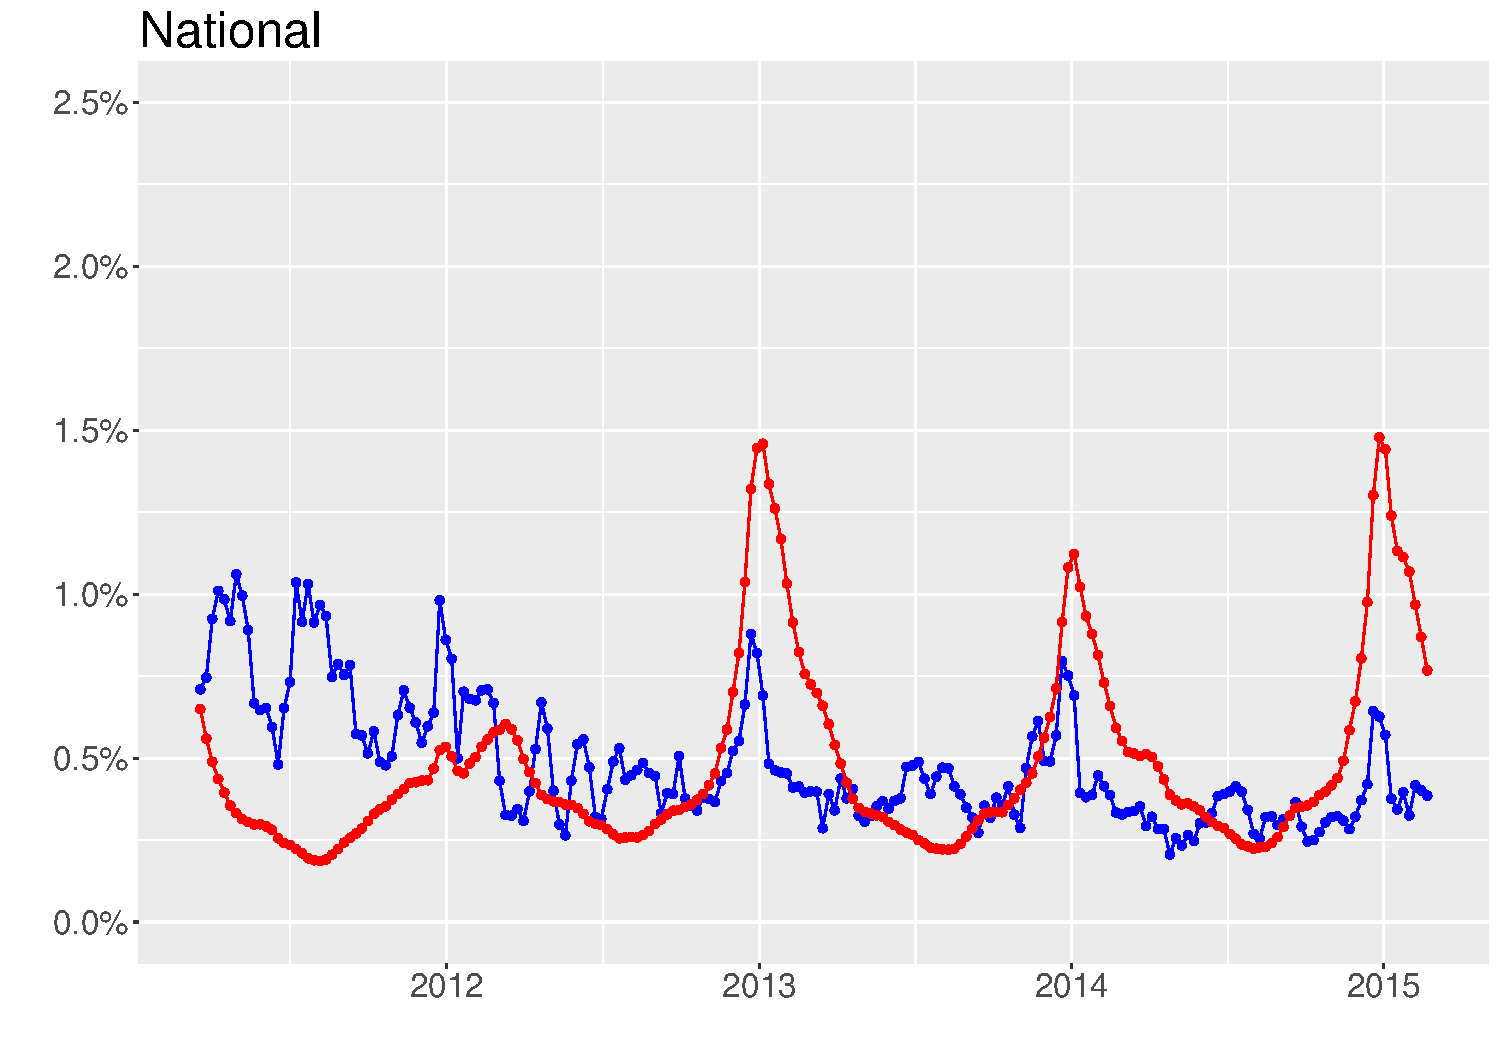
\includegraphics[width=1\linewidth,height=0.5\linewidth]{cdc_twitter_comp_nat_ma4.pdf}
  \caption{}
  \label{fig:cdc_tw_comp_nat_ma4}
  \end{subfigure}
  \caption{Comparison between weekly CDC ILI rates (red) and the relative amount of tweets labelled as ``1 = sick" from the Twitter flu classifier (blue). The data has been normalised in order to make them comparable, i. e. the percentages do not represent weekly ILI percentages, but instead sum up to a 100\% over the whole time period. (a) without smoothing (b) after applying a two-week moving average smoother (c) after applying a four-week moving average smoother}
\end{figure}

\begin{figure}[H]
\centering
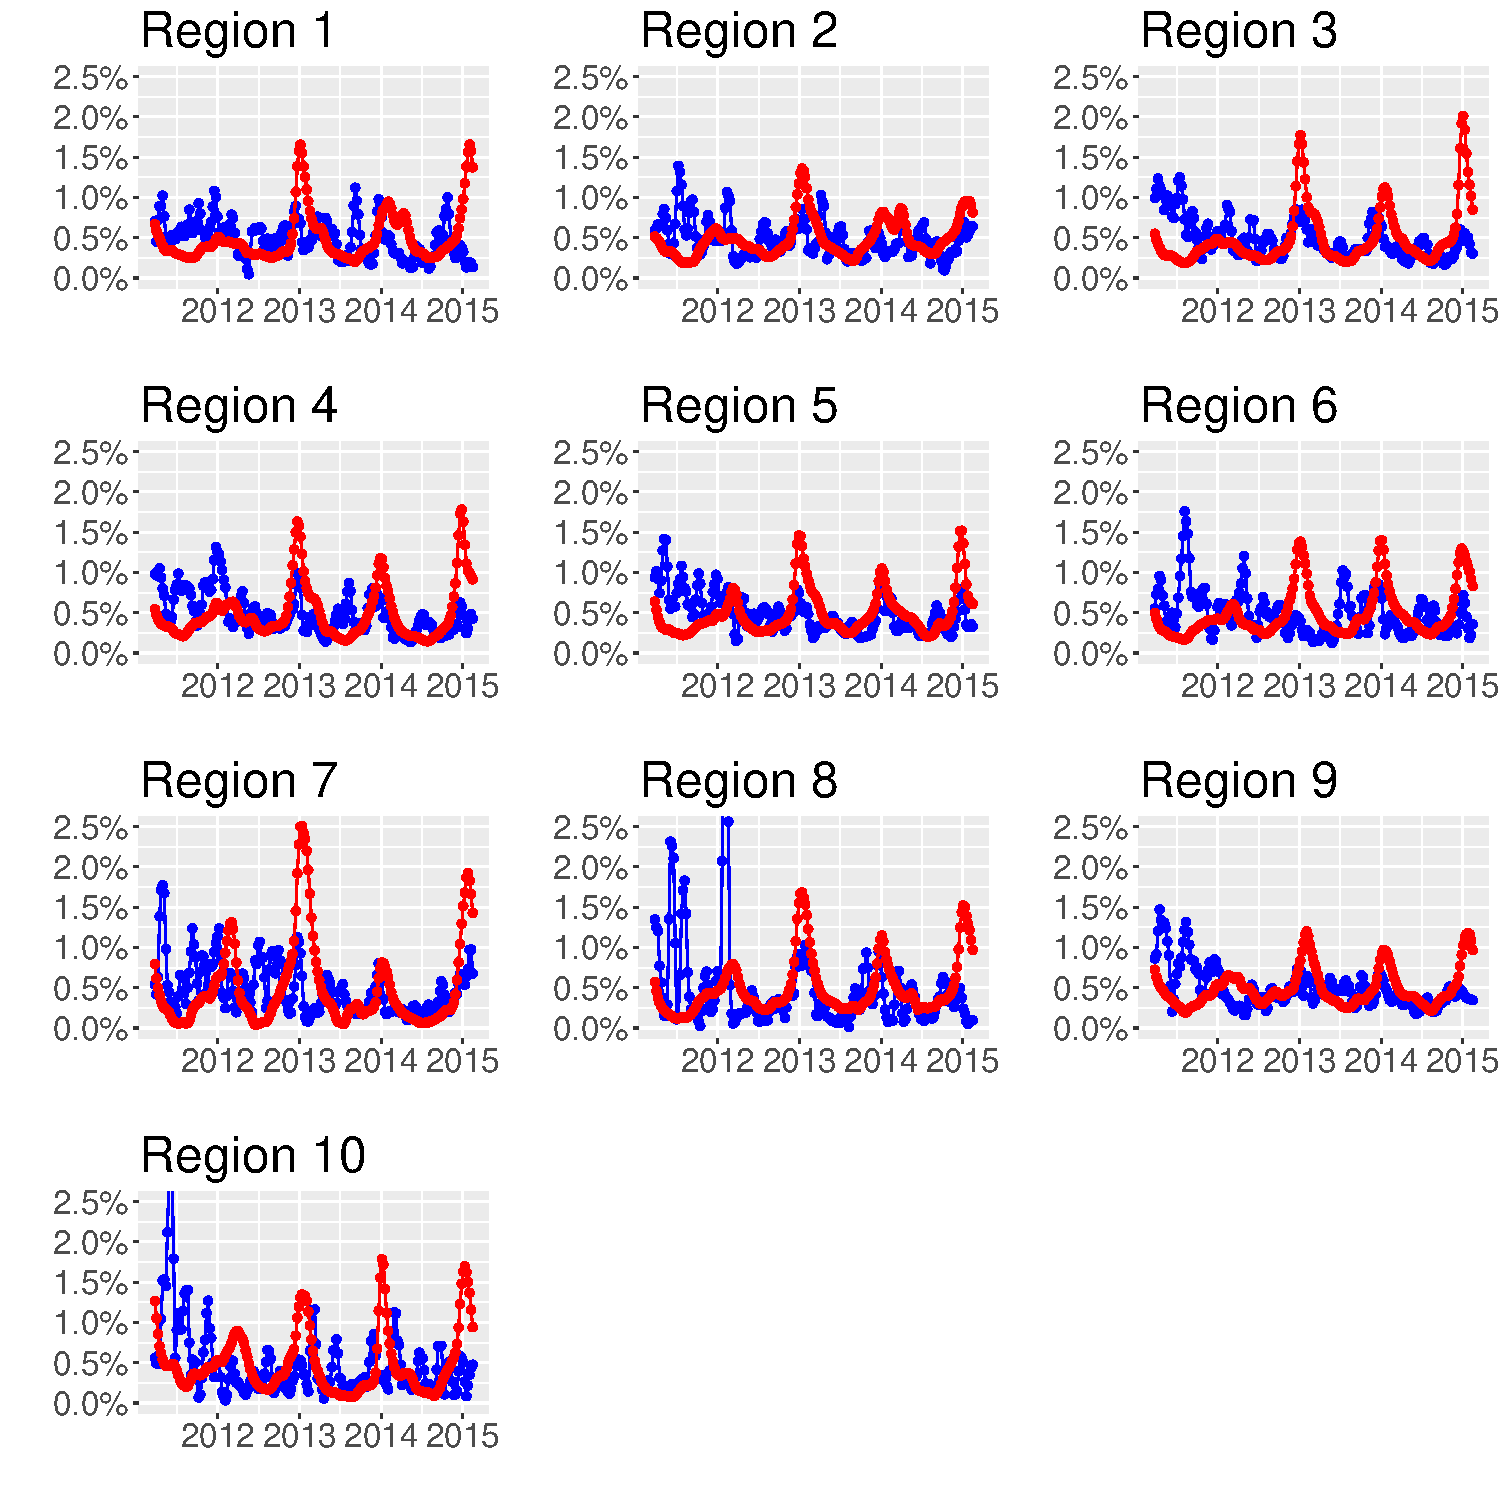
\includegraphics[width=1\linewidth]{cdc_twitter_comp_regs_ma4.pdf}
\caption{Relative number of tweets sent within each CDC ILI surveillance region per week (blue) compared with weekly ILI percentages in those regions (red). Data has been normalised and processed with a four-week moving average smoother. Note that Region 2 contains ``Puerto Rico" and ``Virgin Islands", Region 9 contains ``Hawaii" and Region 10 contains ``Alaska", all of which are missing from the Twitter data set.}
\label{fig:cdc_tw_comp_regs_ma4}
\end{figure}

\begin{figure}[H]
\centering
  \begin{subfigure}[t]{0.6\textwidth}
  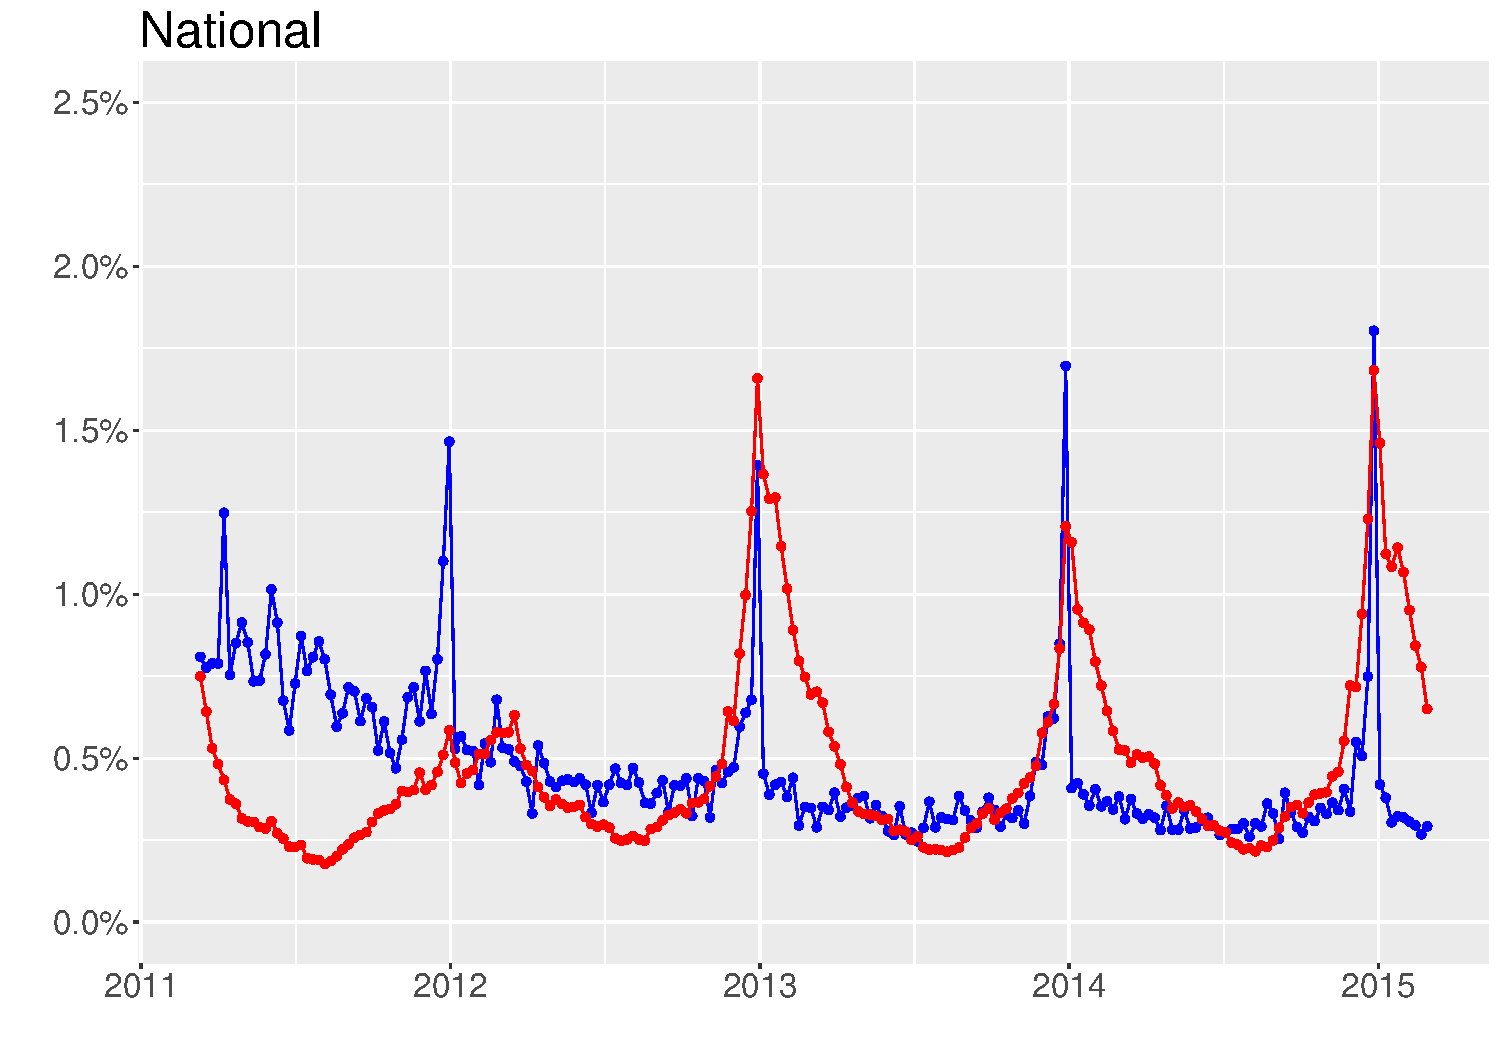
\includegraphics[width=1\linewidth,height=0.5\linewidth]{cdc_twitter_comp_nat_ma1_user.pdf}
  \caption{}
  %\label{fig:cdc_tw_comp_nat_user}
  \end{subfigure}
  
  \begin{subfigure}[t]{0.6\textwidth}
  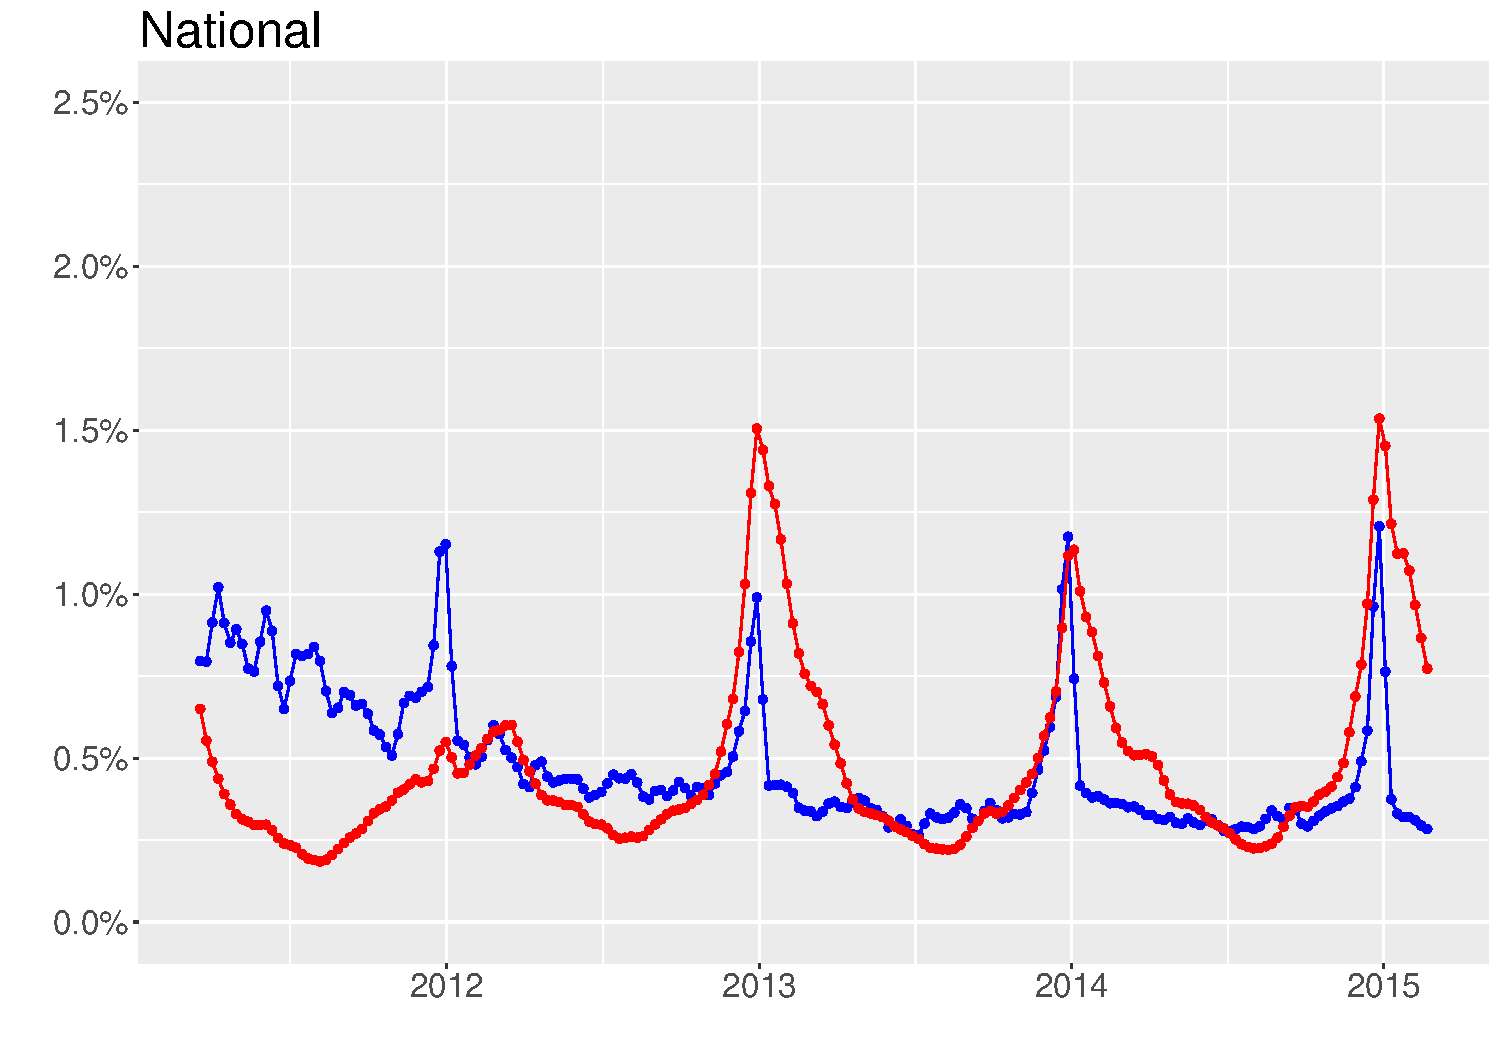
\includegraphics[width=1\linewidth,height=0.5\linewidth]{cdc_twitter_comp_nat_ma2_user.pdf}
  \caption{}
  %\label{cdc_tw_comp_nat_ma2_user}
  \end{subfigure}
  
  \begin{subfigure}[t]{0.6\textwidth}
  \includegraphics[width=1\linewidth,height=0.5\linewidth]{cdc_twitter_comp_nat_ma4_user.pdf}
  \caption{}
  %\label{cdc_tw_comp_nat_ma4_user}
  \end{subfigure}
  \caption{Comparison between weekly CDC ILI rates (red) and the relative amount of users who sent at least one tweet classified as ``1 = sick" from the Twitter flu classifier (blue) during a specific week. The data has been normalised in order to make them comparable, i. e. the percentages do not represent weekly ILI percentages, but instead sum up to a 100\% over the whole time period. (a) without smoothing (b) after applying a two-week moving average smoother (c) after applying a four-week moving average smoother}
  \label{fig:cdc_tw_comp_nat_user}
\end{figure}

\begin{figure}[H]
\centering
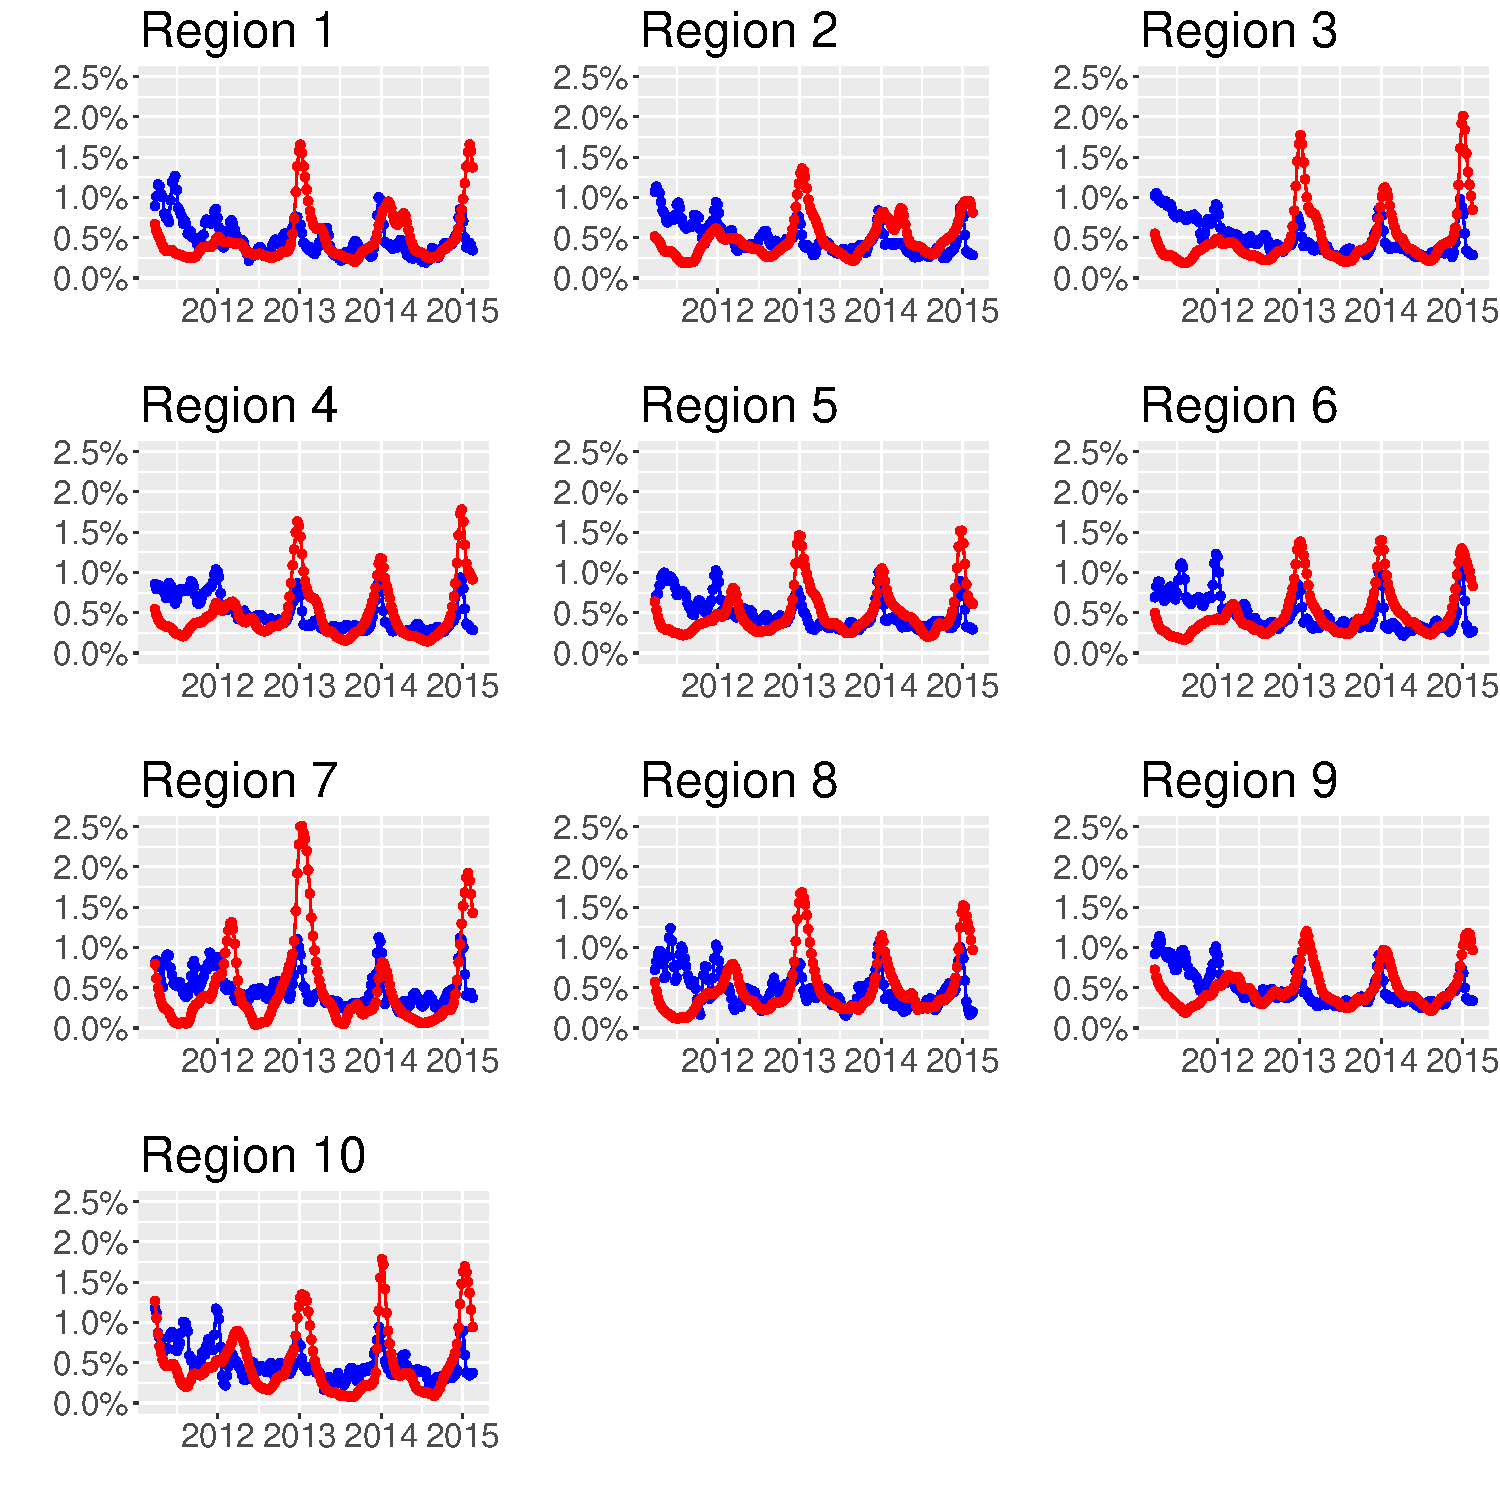
\includegraphics[width=1\linewidth]{cdc_twitter_comp_regs_ma4_user.pdf}
\caption{Relative number of users who sent at least one tweet labelled as ``sick" within each CDC ILI surveillance region per week (blue) compared with weekly ILI percentages in those regions (red). Data has been normalised and processed with a four-week moving average smoother. Note that Region 2 contains ``Puerto Rico" and ``Virgin Islands", Region 9 contains ``Hawaii" and Region 10 contains ``Alaska", all of which are missing from the Twitter data set.}
\label{fig:cdc_tw_comp_regs_ma4}
\end{figure}

\section{Comparison with regard to CDC activity levels}
Next, I attempted to reduce the fluctations and increase the comparibility with the CDC data by grouping the percentual values into one of ten activity levels inspired by the CDC's same grouping used for reporting.\newline

The CDC differentiates between ten different ILI activity levels which represent the deviation relative to the ILI baseline values. The activity levels compare the mean reported percent of visits due to ILI for the current week to the ILI baseline based on the number of reported ILI cases during non-influenza weeks which are defined as weeks with less than 2\% of reported patient visits due to ILI. More precisely, the baseline is calculated by averaging the percentages of recorded ILI patients during non-influenza weeks for the previous three seasons and then adding two standard deviations \citep{cdc_surveillance_2016}.

An activity level of 1 corresponds to values that are below the baseline, level 2 corresponds to an ILI percentage less than 1 standard deviation above the baseline, level 3 corresponds to ILI more than 1, but less than 2 standard deviations above the baseline, and so on, with an activity level of 10 corresponding to ILI 8 or more standard deviations above the baseline \citep{cdc_surveillance_2016}.\newline
  
Since a similar threshold does not exist for the Twitter data, I simply used the relative number of tweets labelled as ``1 = sick" during weeks outside the flu season (June to September; seasonal flu activity can begin as early as October and continue to occur as late as May) as source to calculate yearly baseline values during off-season weeks. I then used these baseline values to calculate the weekly activity levels according to the rationale describe above. Figure~\ref{fig:cdc_tw_comp_nat_ac_sick} and Figure~\ref{fig:cdc_tw_comp_regs_ac_sick} shows the comparison on the national and regional level, respectively. I then did the same using the relative number of sick users (as opposed to sick tweets) instead (Figure~\ref{fig:cdc_tw_comp_nat_ac_sick_user} and Figures~\ref{fig:cdc_tw_comp_regs_ac_sick_user})\footnote{Note that the Twitter data available to me only spanned the time period between 2011 and 2015. In order to data comparable with the official CDC data, I only calculated the baseline based on the off-season weeks directly preceding a specific flu season (as opposed to calculating the baseline based on the off-season weeks of the three preceding weeks)}.\newline

\begin{figure}[H]
\centering
  \begin{subfigure}[t]{0.6\textwidth}
  
\includegraphics[width=1\linewidth]{cdc_twitter_comp_nat_activity_sick.pdf}
    \caption{}
  \label{fig:cdc_tw_comp_nat_ac_sick}
  \end{subfigure}
  
  \begin{subfigure}[t]{0.6\textwidth}
  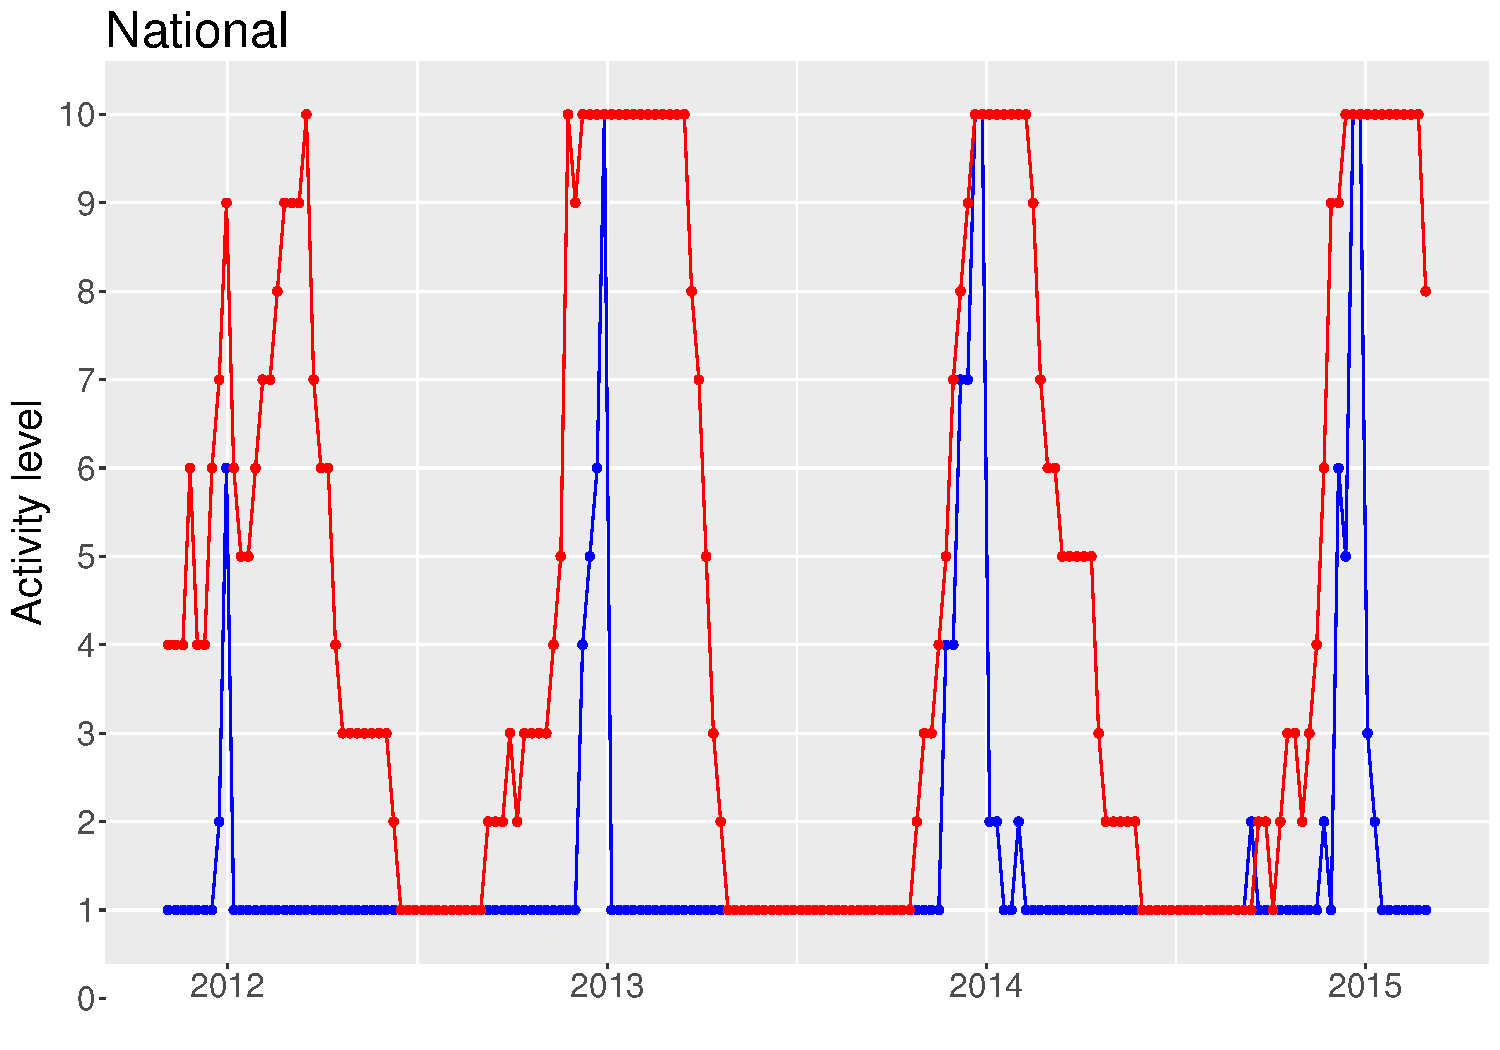
\includegraphics[width=1\linewidth]{cdc_twitter_comp_nat_activity_sick_user.pdf}
    \caption{}
  \label{fig:cdc_tw_comp_nat_ac_sick_user}
  \end{subfigure}
  
  \caption{Comparison between weekly ILI activity levels reported by the CDC and calculated based on the Twitter data set. (a) activity levels based on relative number of sick tweets (b) activity levels based on relative number of sick users}
\end{figure}

\begin{figure}[H]
\centering
  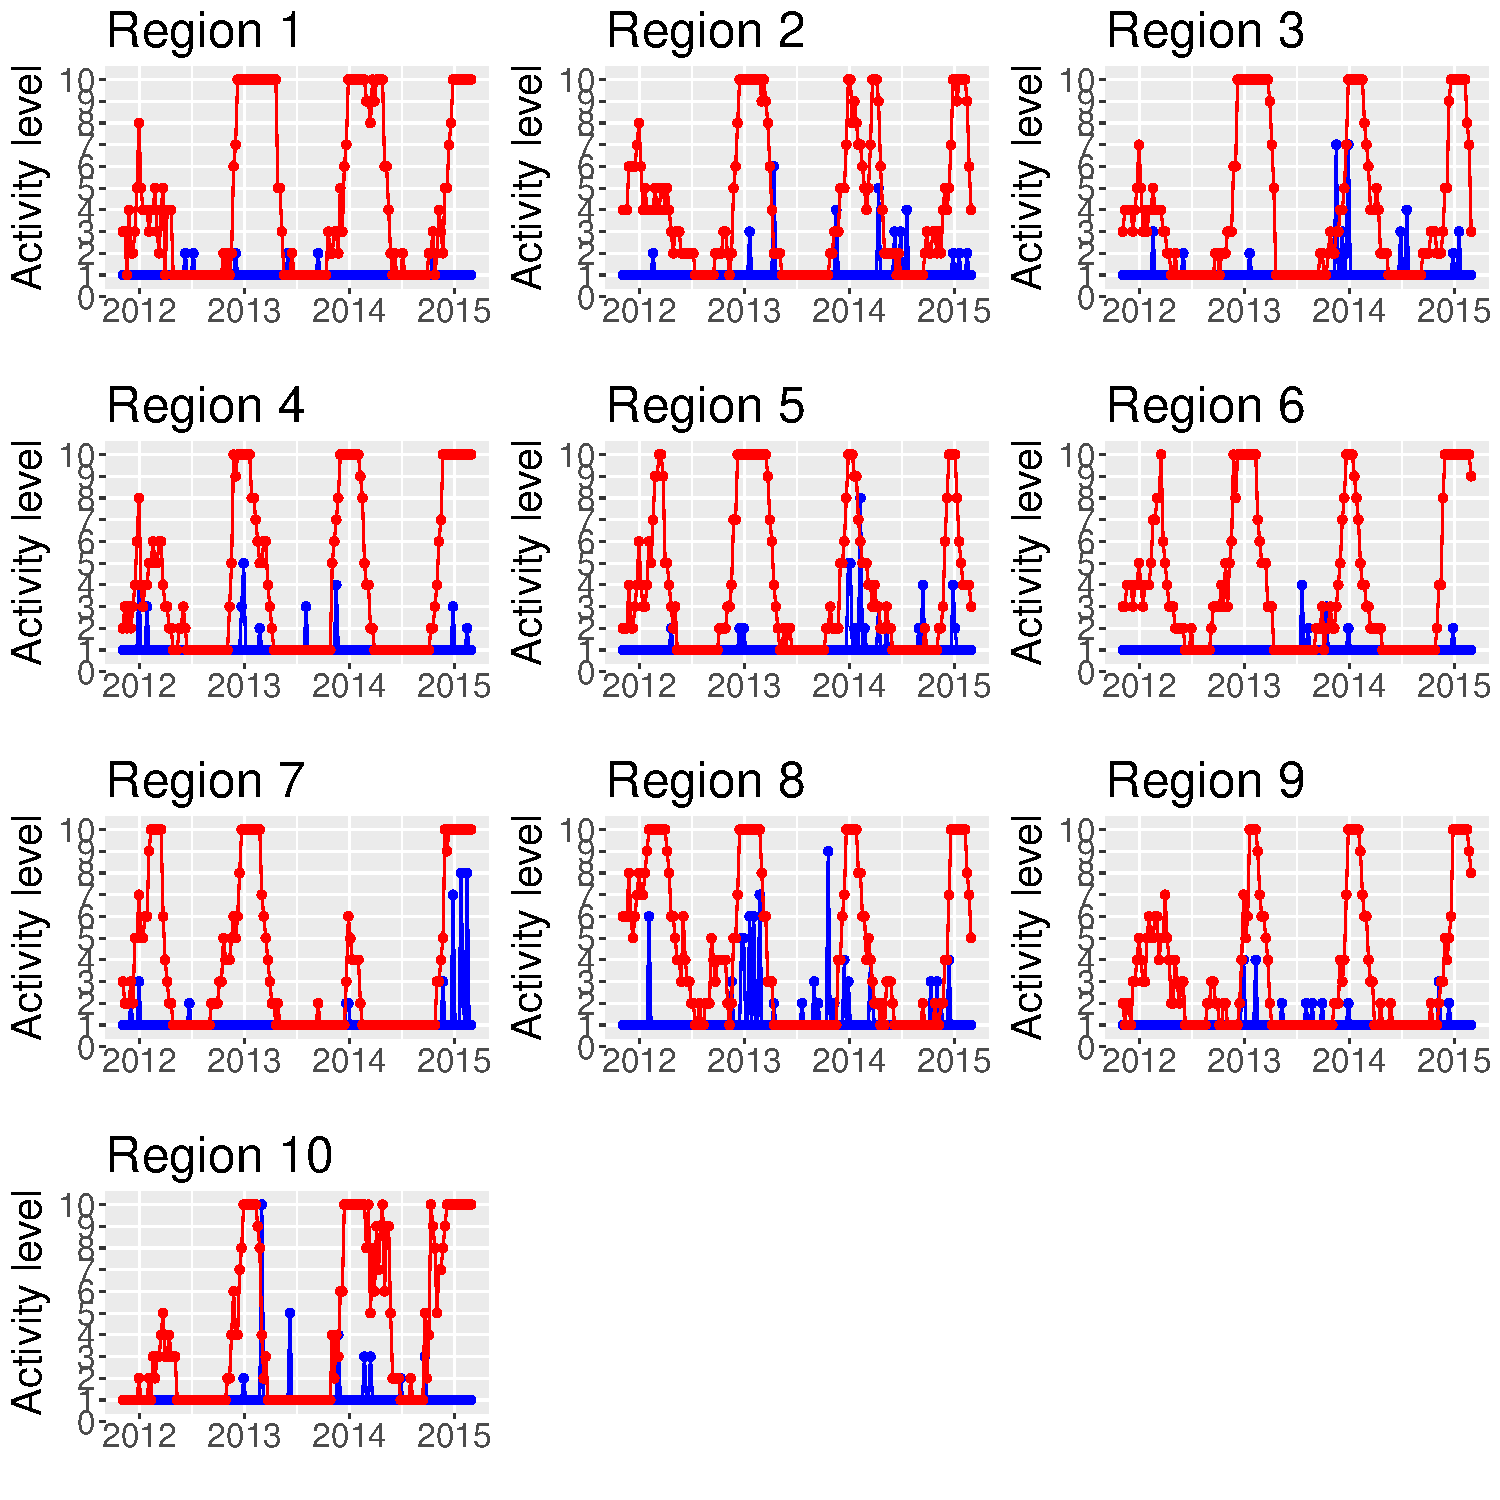
\includegraphics[width=1\linewidth]{cdc_twitter_comp_regs_activity_sick.pdf}
  \caption{Comparison between regional weekly ILI activity levels reported by the CDC and calculated based on relative number of sick tweets per week}
    \label{fig:cdc_tw_comp_regs_ac_sick}
\end{figure}

\begin{figure}[H]
\centering
  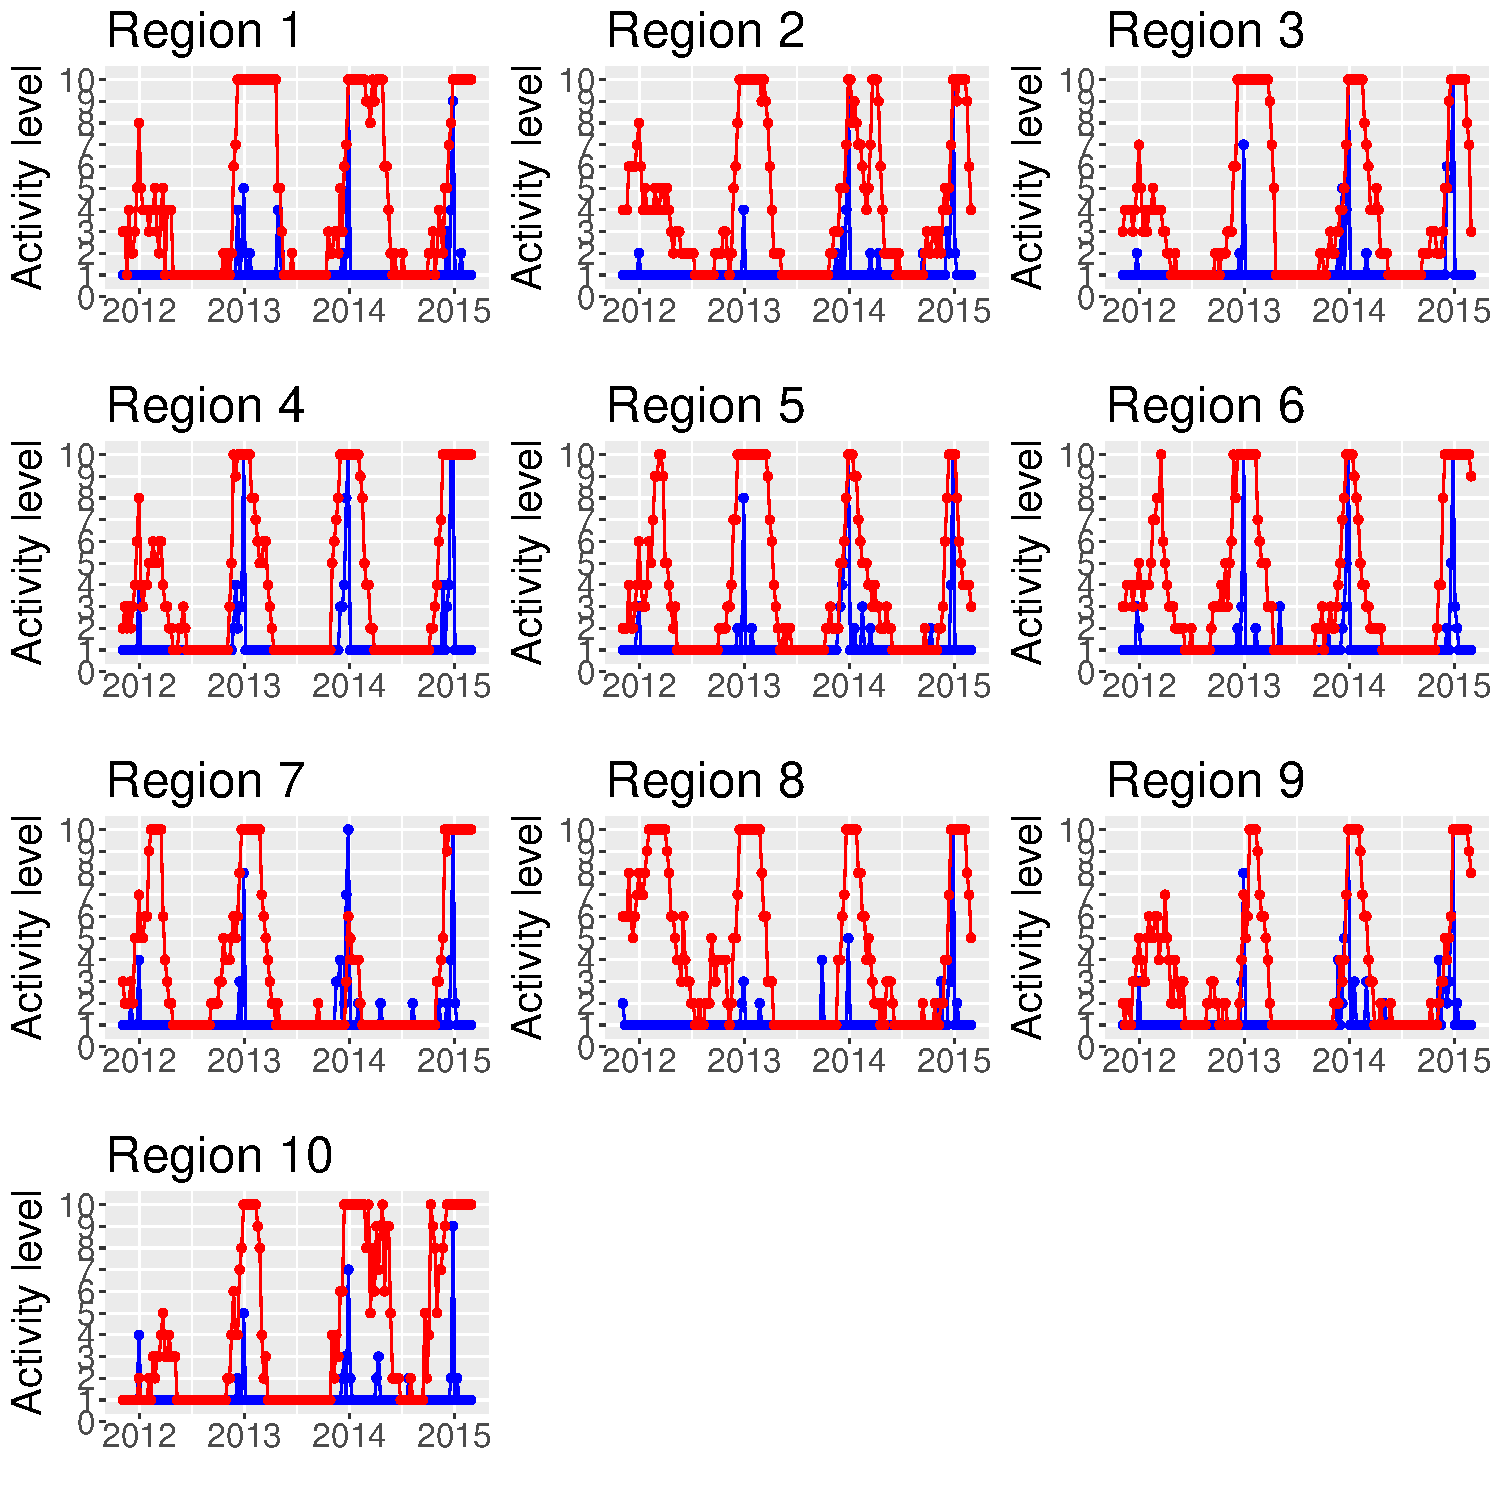
\includegraphics[width=1\linewidth]{cdc_twitter_comp_regs_activity_sick_user.pdf}
  \caption{Comparison between regional weekly ILI activity levels reported by the CDC and calculated based on the relative number of sick users per week}
    \label{fig:cdc_tw_comp_regs_ac_sick_user}
\end{figure}

To get a better understanding of the spatio-temporal pattern of ILI activity levels, I additionally built a function that would take CDC ILI data as well as classified Twitter data and build a map of flu activity over time. The two videos below show the comparison of CDC and Twitter activity levels on a regional level. The first video shows the comparison of activity levels based on the relative number of tweets labelled as sick, the second video shows the comparison of activity levels based on the relative number of sick users per week. White means that CDC and Twitter activity levels are exactly the same, red means that the CDC reported higher ILI activity levels in a given state than those calculated from the Twitter data set, blue indicates the opposite. As can be seen, the Twitter ILI classifier hardly ever manages to emulate the CDC activity levels and when it does, it mainly happens during off-season weeks.\newline

\centering \href{run:vids/regional_Twitter_cdc_diff_full_rel_sick.avi}{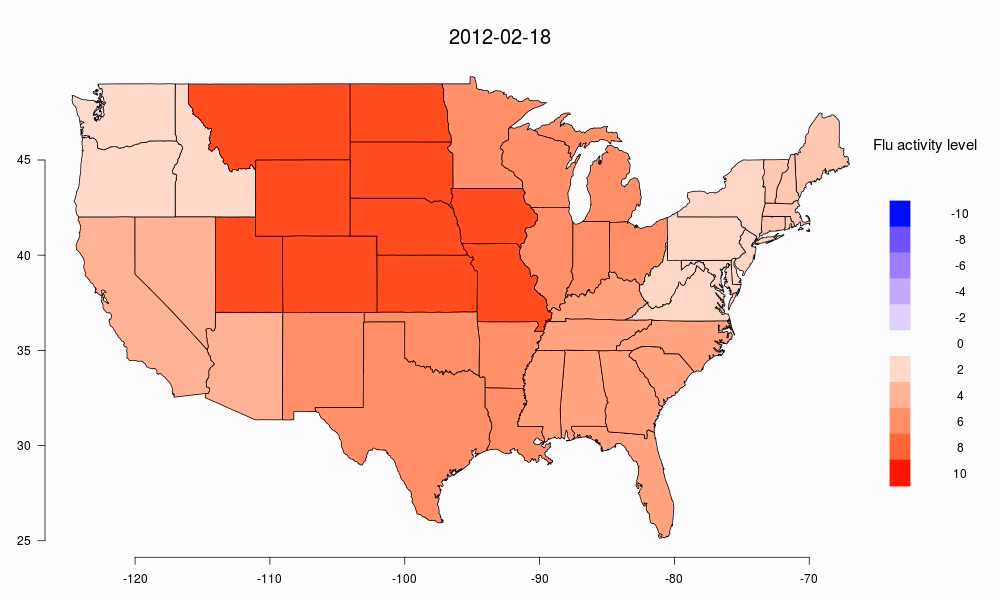
\includegraphics[scale=0.5]{vids/Screenshot_Movie.png}} 

\bigskip

\centering \href{run:vids/regional_Twitter_cdc_diff_full_rel_sick_user.avi}{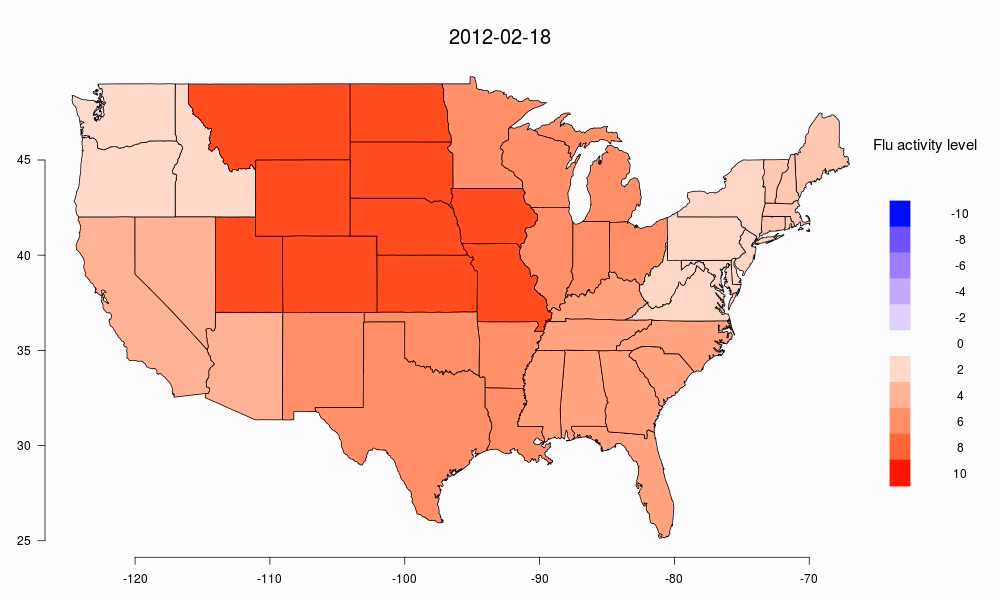
\includegraphics[scale=0.5]{vids/Screenshot_Movie.png}} 

\raggedright

\section{Comparison on the state level}
In a next step, I tried to assess the performance of Twitter flu classifier by looking at state-level data. To do so, I again calculated activity levels for each state and week based on the relative amount of tweets labelled as ``1 = sick" and the relative number of users classified as ``1 = sick", respectively. Due to space reasons and since the fit with the CDC activity curves was worse than for the regional and national data, I did not include the individual time series to this report, but only the two videos showing the spatio-temporal differences in ILI activity levels. The first video contains the comparison with activity levels based on the relative amount of tweets labelled as ``1 = sick" in each state, while the second video contains the comparison based on the relative number of users classified as ``1 = sick" during as specific week and within a given state. Again, it is clear the activity levels based on the Twitter data fit the official CDC only poorly.\newline

\centering \href{run:vids/state_Twitter_cdc_diff_full_rel_sick.avi}{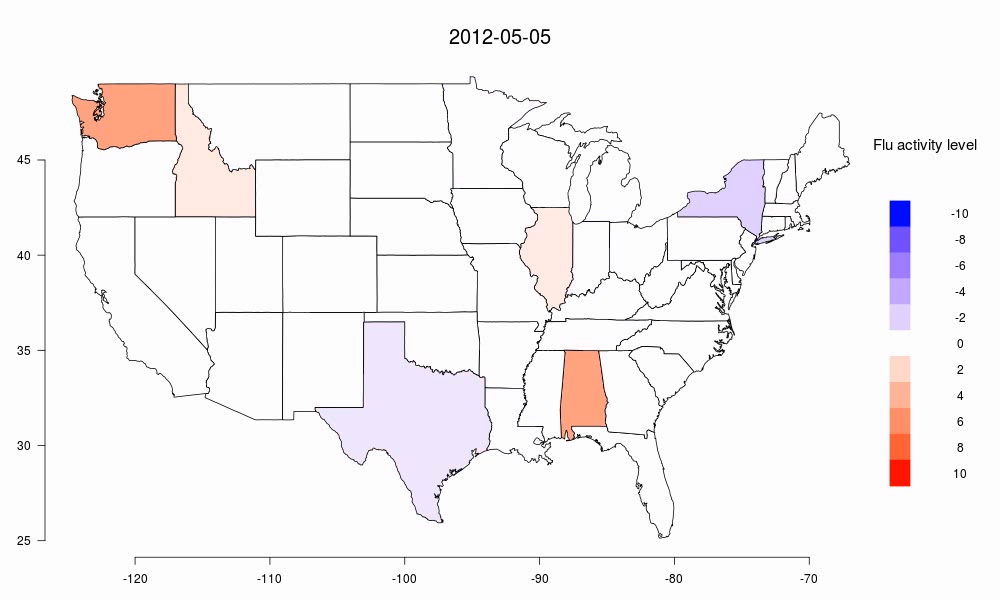
\includegraphics[scale=0.5]{vids/ScreenshotState.png}} 

\bigskip

\centering \href{run:vids/state_Twitter_cdc_diff_full_rel_sick_user.avi}{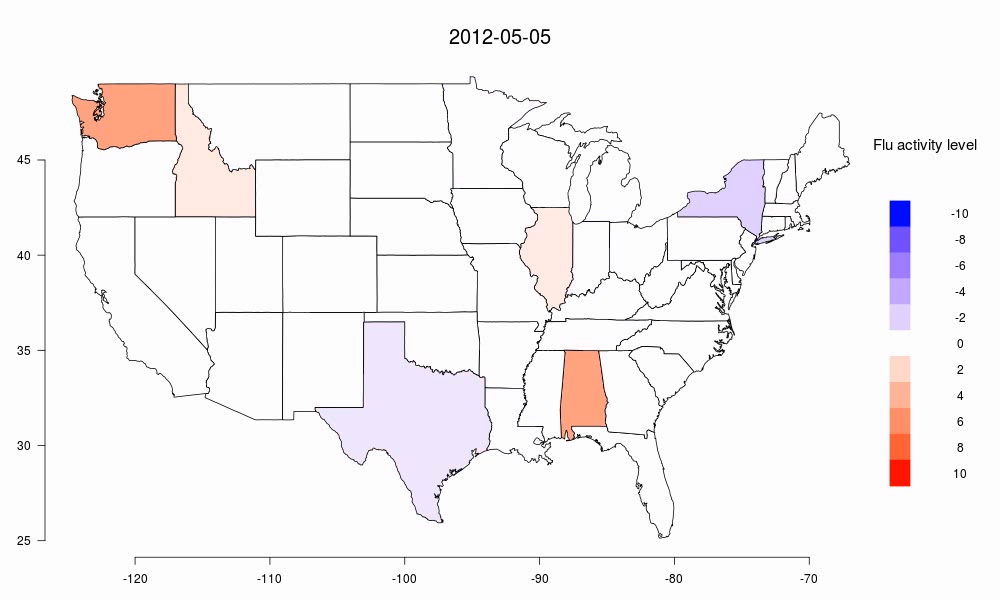
\includegraphics[scale=0.5]{vids/ScreenshotState.png}} 

\raggedright

\section{Comparison on the county level}
In order to assess the performance of the classifier on the county level, I contacted 18 state health departments (Arkansas, California, Florida, Illinois, Iowa, Louisiana, Maine, Michigan, Minnesota, Mississippi, Missouri, New Jersey, New York, North Dakota, Oregon, South Dakota), asking them for their county-level or regional ILI data between 2011 and 2015. I only received the county-level data from the state of Oregon, while the state of California provided me with state-level data only (an official request for county-level data is pending). All other states did either not answer or declined my request. Luckily, the states of New Jersey and Mississippi provided (almost) complete county-level ILI data on their website for the requested time period. Since the data was only provided in pdf-format, I built a scraper for both states in order to retrieve the relevant information.\newline 

Below, you can see the spatio-temporal comparison of the performance of the Twitter flu classifier for the counties of New Jersey (top) and Oregon (below). Note, that Oregon did not provide ILI estimates for all counties (most of the northeastern counties are missing, for example).\newline

\centering \href{run:vids/county_Twitter_cdc_diff_newjersey.avi}{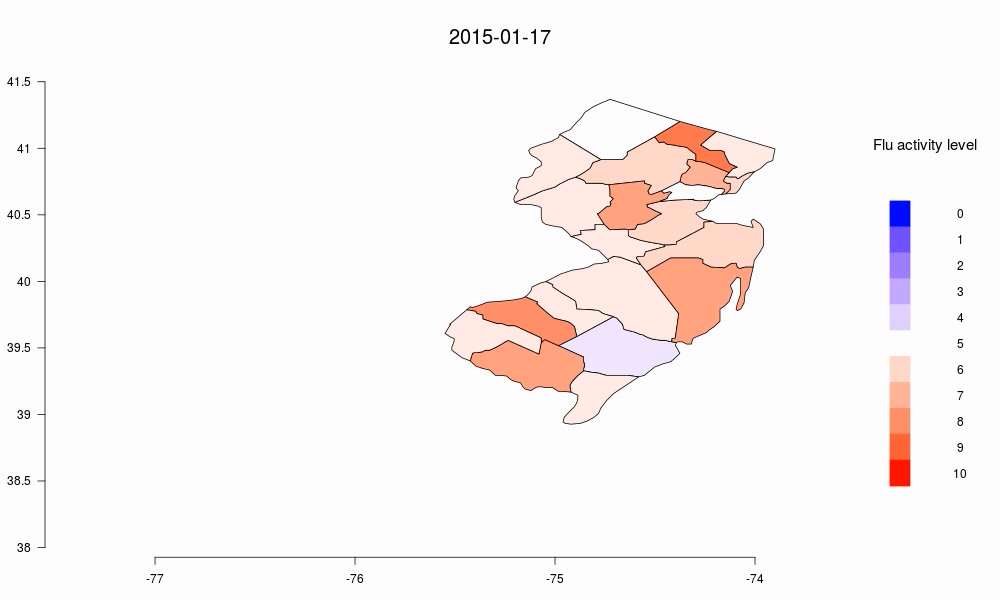
\includegraphics[scale=0.5]{vids/Screenshot_Jersey.png}} 

\bigskip

\centering \href{run:vids/county_Twitter_cdc_diff_oregon.avi}{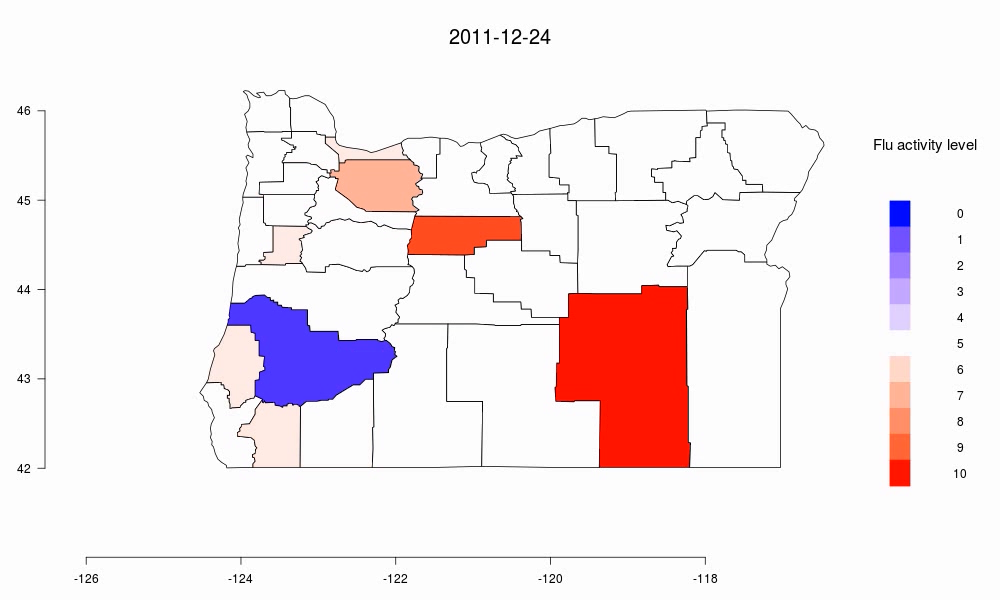
\includegraphics[scale=0.5]{vids/Screenshot_Oregon.png}} 
\raggedright

\section{Additional attempts to reproduce the findings froms \citep{bodnar_data_2015}}
As the results depicted above show, the output from the twitter classifier that served as the basis of my analysis does neither serve as a good approximation of the official CDC data nor does it reflect the results shown in \citep{bodnar_data_2015}. There are various potential reasons for this which I will lay out in Chapter~\ref{ch:discussion}. Before doing so, however, I will summarise additional attempts of mine to replicate the results. \newline

\subsection{Attempt to reclassify raw Twitter data}
As described in Chapter~\ref{ch:data_set_description}, the data set I was working on a data set that contained the output of the Twitter classifier described in Chapter~\ref{ch:intro}. Since there might be discrepancies between this data set and the one used in \citep{bodnar_data_2015}, I wanted to reclassify the geotagged raw Twitter data collected between 2011 and 2015 in order to assess whether these results would diverge from the data set I was working on.\newline

To do so, I retrieved the full Java-based Twitter classifier from Todd Bodnar's Github repository (https://github.com/ToddBodnar/Twitter-Parser). However, some libraries used for building the classifier were missing from the repository, while others (most notably the Amazon Web Services (AWS) SDK for Java: https://aws.amazon.com/de/sdk-for-java/) have in the meantime been superceded by newer vesions which are not backwards compatible with older version and thus incompatible with the Twitter classifier. Even though I managed to retrieve the missing libraries through personal communication with Todd Bodnar and also managed to retrieve the same AWS SDK version that was used for the original version of the Twitter classifier, additional compilation errors remained, so I was unable to compile the classifier.\newline

Finally, I received a compiled version of the Twitter classifier (``TwitterParser.jar") directly from Todd Bodnar, allowing me to circumvent the necessity to debug the original code.  Unfortunately, the jar-file encountered runtime erros when trying to analyse raw Twitter files, both on Ubuntu 16.04.2 LTS as well as on Windows 7. Hence, I still failed to reclassify the raw Twitter data using the Twitter classifier. \footnote{All files belonging to the Twitter classifier, including the compiled version of it, can be found on Github (https://github.com/salathegroup/2016\_TwitterEpi) in the folder ``Twitter\_Parser"}

\subsection{Attempt to reproduce the SIR model described in \citep{bodnar_data_2015}}
Since I was unable to reproduce the original results of the Twitter classifier due to compilation and runtime errors of said classifier, and hence was unable to assess the validiy of the data set I was working on, I went at it from the opposite direction: I started from the final results described in \citep{bodnar_data_2015} and tried to ``reverse engineer" them in order to learn how the excellent fit of the Twitter data with the CDC data came about. Specifically, I focused on chapter 4 of \citep{bodnar_data_2015} and tried to reproduce the findings shown in Figures~\ref{fig:cdc_fit_bodnar_thesis} and \ref{fig:cdc_fit_bodnar_thesis_SIR} as well as Table~\ref{tab:nationalparams}.\newline

In a first step, I asked Todd Bodnar for the data and the code used to create the SIR model as well as the figures. I received an the R-files used to build the SIR model as well csv-files containing the data used to create Figures~\ref{fig:cdc_fit_bodnar_thesis} and \ref{fig:cdc_fit_bodnar_thesis_SIR}  However, I did not receive the R-files or the the model specifications in order to create the data contained in said file from the Twitter data· Hence, I could neither associate the data within these files to the raw results from the Twitter classifier nor to the R-code-files that were provided to me. \footnote{I follow-up e-mail regarding this matter is pending response. Data and code files can be found on Github (https://github.com/salathegroup/2016\_TwitterEpi) in the folder ``PhDThesisBodnar"}.\newline

In order to recreated the figures mentioned above, I used the data available in the file ``predictions\_r\_results.csv", which contained weekly ILI estimates from the CDC as well as additional ILI estimates using different autocorrelation models with or without using the data from the Twitter classifier. The data spanned a four year period, starting on October $3^{rd}$ 2011 (week 40) and ending on September $28^{th}$ 2014 (week 39). The 11 columns contained in the data set have the following meaning:\footnote{Personal communication by Todd Bodnar; as mentioned above, as of this point I do not know how the predictive or retrospective Twitter model relates to the results from the Twitter classifier. An email requesting additional information is pending response}  

\begin{itemize}
  \item \textbf{cdcoffset} The official ILI data from the CDC
  \item \textbf{predictions\_base} The percentage of Twitter users classified as ill based on the predictive base model
  \item \textbf{predictions\_autocor} Predictive AR(1) model based on the ``cdcoffset" data
  \item \textbf{predictions\_autocor2} Predictive AR(2) model based on the ``cdcoffset" data
  \item \textbf{predictions\_both} Predictive AR(1) model based on the ``cdcoffset" data combined with the values from the predictive Twitter base model
  \item \textbf{predictions\_both2} Predictive AR(2) model based on the ``cdcoffset" data combined with the values from the predictive Twitter base model
 \item \textbf{full\_base} The percentage of Twitter users classified as ill based on the retrospective base model
  \item \textbf{full\_autocor} Retrospective AR(1) model based on the ``cdcoffset" data
  \item \textbf{full\_autocor2} Retrospective AR(2) model based on the ``cdcoffset" data
  \item \textbf{full\_both} Retrospective AR(1) model based on the ``cdcoffset" data combined with the values from the retrospective Twitter base model
  \item \textbf{full\_both2} Retrospective AR(2) model based on the ``cdcoffset" data combined with the values from the retrospective Twitter base model
\end{itemize}

For the predictive models, only values between weeks $0$ and $t-1$ were used for model building, for the retrospective models the complete available data was used.\newline

I started with the replication of Figure~\ref{fig:cdc_fit_bodnar_thesis_SIR} and the corresponding parameters. I did so by using the grid-search method described in \citep{bodnar_data_2015}\footnote{``Specifically, we
search through three variables, the two transmission parameters $\gamma$,$\beta$, and S(0), the initial susceptibility rate which may be less than 1 due to innate immunity or previous vaccination. Next, we generate a logarithmically spaced 25 by 25 by 25 grid of potential values over this range. We then set $I(0)$ to be the same as the first infection value in the data and $R(0)$ (sic!). We then solve an SIR model, with each of the parameter combinations." Note tht in the R-code I received the optimisation only happened for $\gamma$ and $\beta$, not for $S(0)$, as desribed. This makes intuitive sense: Since we know the initial value of $I(0)$ both for the CDC data as well as for the Twitter model, there is no need to algorithmically find the initial value of $S(0)$, since it can simply be calculated as $S(0)=1-I(0)$, while $R(0)=0$. Indeed, this is exactly the way the initial values were set in the algorithm.}\newline

First, I built the SIR model based on the CDC data, since this was the most straightforward way to go. As can be seen from Figure~\ref{fig:SIR_comparison_CDC}, the yearly and combined ILI curves calculated from the model are very similar to the ones depicted in Figure~\ref{fig:cdc_fit_bodnar_thesis_SIR}, however small deviations remain.\newline

Therefore, I went on to fit the very same SIR model that is shown in Figure~\ref{fig:cdc_fit_bodnar_thesis_SIR}. To do so, I needed to know which data the model was built on. I extracted the three starting coordinates of the yearly curves shown in the figure and compared them with the data provided to me by Todd. It turned out that the starting coordinates of the curve only matched the values from the full retrospective Twitter model (i.e. retrospective AR(2) model based on the CDC data combined with the retrospective Twitter base model), so built my second SIR model based on these values. As can be seen from Figure~\ref{fig:SIR_comparison_full}, the resulting yearly and combined ILI curves are virtually indistinguishable from the ones shown in \citep{bodnar_data_2015}.\newline

\begin{figure}[H]
\centering
  \begin{subfigure}[t]{0.65\textwidth}
  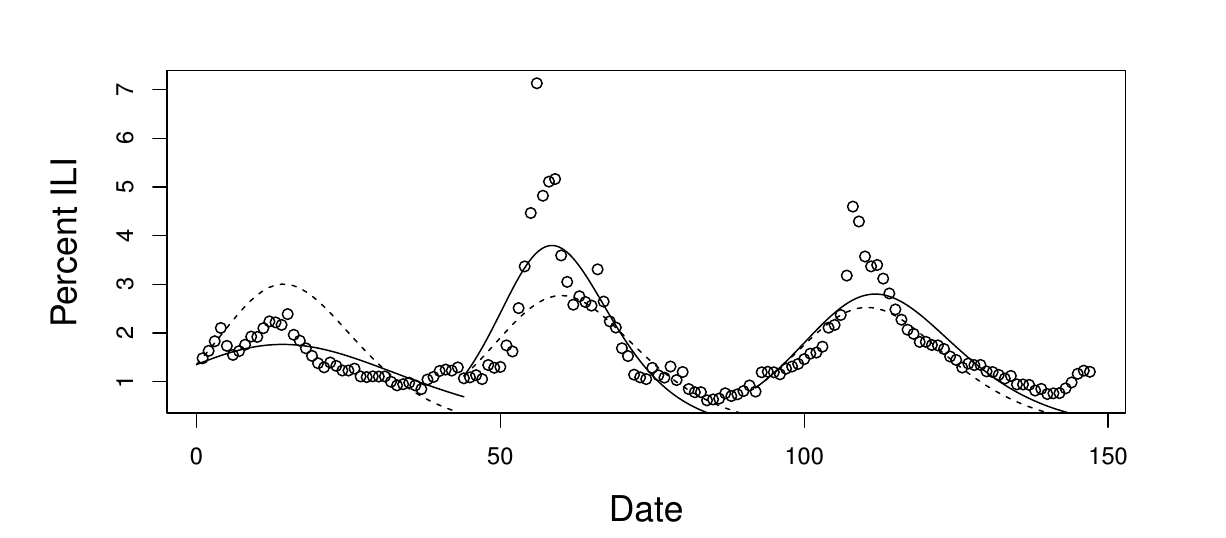
\includegraphics[width=1\linewidth,height=0.5\linewidth]{todd_bodnar_SIR.png}
  \caption{}
  \label{fig:SIR_comparison_original}
  \end{subfigure}
  
  \begin{subfigure}[t]{0.6\textwidth}
  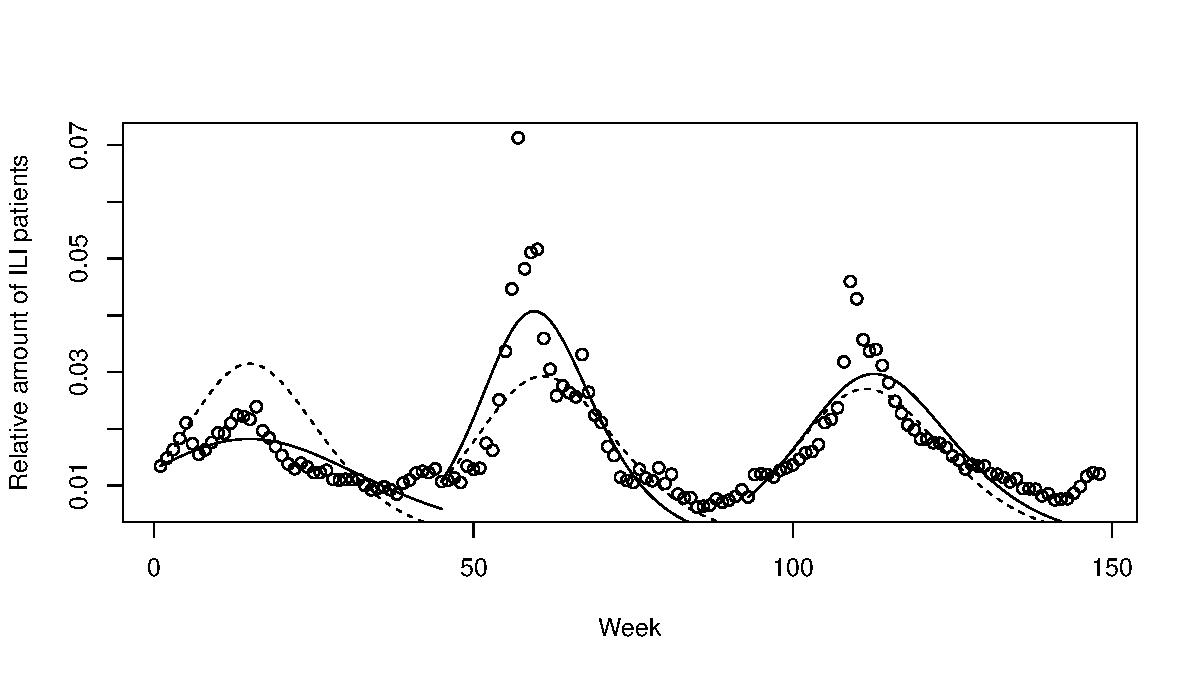
\includegraphics[width=1\linewidth,height=0.5\linewidth]{SIR_model_cdc_data_25.pdf}
  \caption{}
  \label{fig:SIR_comparison_CDC}
  \end{subfigure}
  
  \begin{subfigure}[t]{0.6\textwidth}
  \includegraphics[width=1\linewidth,height=0.5\linewidth]{SIR_model_full_model_25.pdf}
  \caption{}
  \label{fig:SIR_comparison_full}
  \end{subfigure}
  \caption{Comparison between the SIR model depicted in \citep{bodnar_data_2015} (a) and replications based on the official CDC ILI rates (b) and the full retrospective Twitter model (c).}
  %\label{fig:SIR_comparison}
\end{figure}

It is very peculiar, however, that the model parameters which I calculated for the two replicated SIR models described above do not match the yearly and combined values for $\gamma$ and $\beta$ presented in \citep{bodnar_data_2015} - even though model curves seem to match. As can be seen from Table~\ref{tab:nationalparams_replicated}, the optimal yearly and combined values of $\gamma$ and $\beta$ deviate considerably from the ones depicted in Table~\ref{tab:nationalparams} (i.e. the values reported in \citep{bodnar_data_2015}). This is true for the SIR model based on the CDC data as well as for the SIR model based on the full retrospective model data. Hence, it is safe to assume that those values do \textbf{not} represent the values that were used to calculate the curves shown in Figure~\ref{fig:cdc_fit_bodnar_thesis_SIR}.\newline

 \begin{table}[H]
\centering
\begin{tabular}{l l l l l}

 Year & \(\gamma\) & \(\beta\) & RSS\\ \hline
& 0.3962286 & 0.4446748  & \ensuremath{4.0608281\times 10^{-4}}   \\ 
 {\multirow{-2}{*}{ 2011-2012 }}  & \cellcolor{grey}0.3666311  & \cellcolor{grey}0.4087479 & \cellcolor{grey}\ensuremath{3.6266689\times 10^{-4}}  \\ \cline{2-4}
  {\multirow{2}{*}{ 2012-2013 }}& 0.5121045 & 0.6777425  & 0.0029532  \\ 
   & \cellcolor{grey}0.5021989  & \cellcolor{grey}0.6546756 & \cellcolor{grey}0.0027735   \\ \cline{2-4}
  {\multirow{2}{*}{ 2013-2014 }}& 0.451297 & 0.5699723    & 0.0014841   \\ 
   & \cellcolor{grey}0.4294719 & \cellcolor{grey}0.535259 & \cellcolor{grey}0.0013076  \\ \cline{2-4}
  {\multirow{2}{*}{ Combined }}& 0.4878438 & 0.6068527 & 0.008631   \\ 
   & \cellcolor{grey}0.4641424  & \cellcolor{grey}0.5698395  & \cellcolor{grey}0.0077089   \\ 
\end{tabular}
\caption{National best-fit parameters for each year from the CDC's data (white) and the full retrospective model consisting of a retrospective AR(2) model based on the CDC data and the retrospective Twitter base model (grey)}
\label{tab:nationalparams_replicated}
\end{table}

In addition, it is important to note again that the data used to calculate the SIR models is \textbf{not} equivalent to the raw results of the Twitter classifier. In fact, the SIR models described above are built on the full retrospective model data which includes the information from the Twitter classifier as well as information from an AR(2) model based on the official CDC data. This stands in contrast to the report in \citep{bodnar_data_2015}, where the SIR models are depicted as being based on the information from the Twitter classifier only. However, this cannot be the case. Figure~\ref{fig:TwitterModel_comparison} clearly shows that the SIR model built solely on the data from the Twitter base model is clearly distinct from the SIR models built on the full retrospective model data.  

\subsection{Attempt to reproduce the AR model described in \citep{bodnar_data_2015}}
Finally, I tried to reproduce the results depicted in Figure~\ref{fig:cdc_fit_bodnar_thesis}. The graph is described as the ``comparison of Twitter's forecasting (dashed lines) and retroactive measurements (solid lines) to the CDC's reported Influenza rates (circles)", therefory implying that the dashed and solid lines are produces based on the data from the Twitter classifier alone. However, this is clearly not the case. Figure~\ref{fig:TwitterModel_comparison_original} shows a reproduction of the original graph depicted in \citep{bodnar_data_2015}, including SIR model fits. However, this reproduction is based on the retrospective \textbf{full} model, i.e. a model including information from the Twitter base model as well as from the AR(2) model based on the CDC data. In fact, if we only look at the data from the Twitter base model (Figure~\ref{fig:TwitterModel_comparison_base_model}), we can see that the fit with the official CDC data is much worse. Also, Figure~\ref{fig:TwitterModel_comparison_AR2} shows that a simple AR(2) model based on the official CDC data achieves a model fit that is almost as good as the one from the full model which additional includes information from the Twitter base model.

\begin{figure}[H]
\centering
  \begin{subfigure}[t]{0.65\textwidth}
  \includegraphics[width=1\linewidth,height=0.5\linewidth]{SIR_model_full_both_25_colorised.pdf}
  \caption{}
  \label{fig:TwitterModel_comparison_original}
  \end{subfigure}
  
  \begin{subfigure}[t]{0.6\textwidth}
  \includegraphics[width=1\linewidth,height=0.5\linewidth]{SIR_model_full_AR2_100_colorised.pdf}
  \caption{}
  \label{fig:TwitterModel_comparison_base_model}
  \end{subfigure}
  
  \begin{subfigure}[t]{0.6\textwidth}
  \includegraphics[width=1\linewidth,height=0.5\linewidth]{SIR_model_full_base_model_100_colorised.pdf}
  \caption{}
  \label{fig:TwitterModel_comparison_AR2}
  \end{subfigure}
  \caption{Comparison between the full retrospective Twitter model depicted in \citep{bodnar_data_2015} (a) and replications consisting of a simple retrospective AR(2) model based only on CDC ILI rates (b) and the retrospective Twitter base model (c)}
  \label{fig:TwitterModel_comparison}
\end{figure}

\chapter{Discussion}
\label{ch:discussion}
The failure to replicate the findings from \citep{bodnar_data_2015} can have multiple reasons: 

\begin{itemize}
\item Coding errors distoring the aggregation and analysis of the Twitter data set
\item The findings from \citep{bodnar_data_2015} are based on a different data set
\item There are errors present in the Twitter classifier code
\item The findings can only be replicated by using the classified tweets as a starting point for more intricate models
\end{itemize}

I shortly will address each one of these steps in the following passages and explain what I have done to address them during my thesis. 

\section{Errors in the aggregation and processing of the Twitter data set}
This is the most obvious, but also most frequent source of errors to occur. Handling huge data sets does not only put a strain on the computer's hardware, but also on the computer user's software, since it requires a different way of handling, aggregating and manipulating data sets in order to prevent memory overflow errors or calculation that take until the end of the universe to finish.\newline

It should not come as surprise, though, that very often in the course of this thesis I have been forced to rewrite various parts of my code or try to find a new a approach to a specific problem. It has occurred very often, too, that seemingly nonsensical code output could quickly be fixed by finding the misplaced column index or the redundant loop.\newline

This also the reason, however, for which I am fairly confident that the results reported in this thesis do not contain any errors based on faulty code. For almost every step in the description, aggregation and analyis of the data I have usually chosen at least two different approaches (not all of them are reported in this thesis, but all the complete code source and all results are available on Github) Partially, because I usually encountered better methods along the way, partially because I wanted to have a control for my code in order to prevent any unintentional mistakes. Barring any obscure bugs in the packages I used (which seems extremely unlikely), the failure to reproduced the findings from \citep{bodnar_data_2015} should not stem from any coding errors. Nevertheless, the code set I generated is comparable large and not at all as clean and simple as I wished it to be, thereby also increasing the probability for unwanted errors sneaking in. Hence, the in order to make this thesis as resproducible as possible and in order to facilitate any follow-up analysis, I will further clean up the code and the database structure.\newline

\section{The findings from \citep{bodnar_data_2015} are based on a different data set}
As written in the Chapter~\ref{ch:data_set_description}, there is ample evidence that the data set I used was not identical to the one used in \citep{bodnar_data_2015}. Basic statistical properties such as the average tweet rate, total number of sick users or total number of users were considerably different. One reason for this could be that the data set I analysed was processed by a different Twitter classifier. This is not too unlikely, since Todd Bodnar described several different flu classifiers in his thesis, of which apparently only one was used to fit to the official CDC data. Nevertheless, personal e-mail correspondance with Todd Bodnar in fact confirmed that the data set described in his thesis and the one stored in the data base dumps of the Salathé research group were in fact the same. In this case, the only explanation would be that the data set was inadvertently changed at some point after the end of this thesis.\newline

\section{There are errors present in the Twitter flu classifier}
This is an idea that I entertained early on and that was in fact the original starting point of this thesis: The attempt to replicate the Twitter flu classifier analysis in a first step in order to improve it in a second step.\newline

However, in order to assess the quality of and improve said Twitter flu classifier one would not only need access to it, but also get it up and running. Unforunately, I was unable to reclassify the Twitter data in order to confirm my assumptions due to missing / deprecated libraries and runtime errors in the Twitter classifer, respectively. Hence, debugging and updating the Twitter classifier should be a main goal for future replication attempts.\newline

\section{The findings can only be replicated by using the classified tweets as a starting point for more intricate models}
In my eyes, this is the most likely explanation for the abysmal fit between the Twitter data and the official CDC data. In fact, \citep{paul_worldwide_2015} report that autoregressive models of CDC data are very strong baseline models and in general better than twitter models alone. This shows that Twitter cannot predict CDC ILI rates on its own but should rather be used as an additional source of information to complement already existng estimates and reduce the error. As I have shown in Chapter~\ref{ch:results}, this also true for the Twitter data used in \citep{bodnar_data_2015}: The Twitter base model alone was not able to fit the official CDC data tightly and was clearly outperformed by a simple AR(2) model based on the official CDC data. \newline

Also, \citep{paul_twitter_2014} report that most disease models are using \textbf{revised} CDC data which are already corrected for mistakes. However, Twitter data might be much more useful when used with unrevised data instead. In addition, \citep{aramaki_twitter_2011} report that Twitter data is most useful for the early detection of influenze epidemics, but could be rather rather sensitive to excessive news periods revolving around the flu.\newline

Hence, using the Twitter data to fit a model to the official CDC data does certainly improve the fit between the Twitter flu predictions and the official CDC ILI data. However, this then again opens up the classifier to the perils of overfitting and would entirely defeat the purpose of building a classifier which is \textbf{independent} of population-level ILI data. \newline

In fact, \citep{bodnar_data_2015} fitted an SIR model to the results from the Twitter flu classifier in order to compare results. However, he reported that the model had to be refitted for every individual year based on the official CDC data (again, defeating the purpose of having a classifier independent of population level data). Also, the model fit was much lower (see Figure~\ref{fig:cdc_fit_bodnar_thesis_SIR}) and in no way comparable to the extraordinary fit shown in Figure~\ref{fig:cdc_fit_bodnar_thesis}). In the meantime, I received the code used to fit the SIR model as well as the data used to produce Figure~\ref{fig:cdc_fit_bodnar_thesis}. However, it as of yet unclear to me how exactly this data was produced based on the model parameters fitted in the SIR model. An answer to a follow-up e-mail to Todd Bodnar with regard to this is currently pending.\newline

In any case, however, the discrepancies between the model fits described in \citep{bodnar_data_2015} and the results presented in Chapter~\ref{ch:results} of this thesis are worrying. Whatever the reason may be, it is clear that the information from the Twitter classifier on its on cannot be used to reliably predict CDC ILI rates. Even when disregarding the raw results from the raw Twitter classifier (described in ~\ref{ch:data_set_description}) and only focusing on the (processed) data that supposedly served as basis for \citep{bodnar_data_2015}, many unpleasant discrepancies are found that. It seems as if the models relying on the results from the Twitter classifier are widely outperformed by a simple AR(2) model based on the CDC data.

\section{Missing parts}

\begin{itemize}
\item Formatting and citations
\item Cleaning up code \& repository (> any specific guidelines to follow for this?)
\end{itemize}

\newpage
% \nocite{R}
\bibliographystyle{mywiley}
\bibliography{Masterarbeit.bib}

\newpage
\bibliographystylepackages{mywiley}
\bibliographypackages{RPackages.bib}


%\bibliography{Consulting}
%\printbibliography

\vfill

\footnotesize

{\bf \prog{R} version and packages used to generate this report:}

\prog{R} version: \textsf{R version 3.4.1 (2017-06-30)}

Base packages: \textsf{stats, graphics, grDevices, utils, datasets, methods, base}

Other packages: \textsf{data.table, knitr}

This document was generated on August 12, 2017 at 15:23.



\end{document}




